% !TEX root = ../main.tex
\fancychapter{Evaluation}%
\label{chap:eval}
\cleardoublepage{}

\noindent In this chapter, we evaluate our solution by measuring the qualities
of the approach we took to tackle \ac{GCS}.

Firstly, we aim to benchmark our solution's performance by comparing it to a
similar project called ConstraintGM~\cite{Pinheiro:2016:MGR}.  We were able to
reproduce the project's original benchmark tests and create an analogous test
suite for our solution so we can compare both projects.

Secondly, we showcase four different case studies inspired by existing designs.
This section of the evaluation focuses on comparing different approaches to
solving \ac{GC} problems present in each case study by adopting two different
approaches: 
\begin{enumerate*}[label= (\arabic*)]
  \item an analytic approach, one programming naturally begs for, and 
  \item a constructive approach, essentially adding a conceptual abstraction
  layer over the former.
\end{enumerate*}
We aim to show that, by following the latter approach, resulting programs become
both easier to understand and reproducible as the set of instructions can be
used to recreate the resulting geometry by hand, using a ruler and a compass.

Finally, as an added bonus, we explore our approach's potential regarding
repurposing more complex geometric algorithms, contrasting it with
re-implementing a version of said algorithms from scratch.  Specifically, we set
out to repurpose \ac{CGAL}'s 2D Delaunay Triangulation and Voronoi Diagram
algorithms and further compare the resulting mapping's performance and
correctness when compared to a native Julia implementation of the algorithms as
provided by the package
\texttt{VoronoiDelaunay.jl}\footnote{\url{https://github.com/JuliaGeometry/VoronoiDelaunay.jl}},
that, in the past, was once benchmarked against
\ac{CGAL}.\footnote{\url{https://gist.github.com/skariel/3d2018f9341a058e00fc}}
Additionally, we set out to estimate the effort it took to develop
\texttt{VoronoiDelaunay.jl} and compare that to the effort it took to extract an
analogous algorithm from \ac{CGAL}.

Benchmarks were performed on a Lenovo{\textregistered}
ThinkPad{\textregistered} E595 laptop computer with the following
system specifications:

\begin{itemize}
  \item \acsu{AMD}\label{acro:AMD} Ryzen\textsuperscript{\texttrademark} 5 3500U
  \acsu{CPU}\label{acro:CPU} @ 2.1GHz\footnote{Base clock frequency.  Can boost
  up to 3.7GHz.}
  \item 1×16GB \acsu{SO-DIMM}\label{acro:SO-DIMM} of \acsu{DDR}\label{acro:DDR}4
  \acsu{RAM}\label{acro:RAM} @ 2400MT/s
  \item Arch
  Linux\textsuperscript{\texttrademark}\footnote{\url{https://archlinux.org}}
  x86 64-bit, Linux{\textregistered} Kernel
  5.12.15-zen1\footnote{\url{https://github.com/zen-kernel/zen-kernel/tree/v5.12.15-zen1}}
\end{itemize}
\clearpage

% !TEX root = ../../main.tex
\subsection{ConstraintGM}%
\label{sec:eval.cgm}

ConstraintGM is a domain-specific language developed with the goal of tackling
\ac{GC} problems using the Racket \ac{TPL}.  This solution blindly relied on
Maxima~\cite{Maxima:2021:Maxima}.

This approach came at a grave performance cost for two reasons:
\begin{enumerate*}[label= (\arabic*)]
  \item the communication between ConstraintGM and Maxima was slow, and
  \item Maxima is a \emph{generic} solver.
\end{enumerate*}
The considerable performance penalty of this approach is hard to justify in the
case of simple geometric problems. This lead to the implementation of some
\ac{GC} problem solutions, creating the \ac{GFL}.

The project's benchmark involved three different \ac{GC} problems focused around
object intersection, namely
\begin{enumerate*}[label= (\arabic*)]
  \item line-line intersection,
  \item circle-line intersection, and
  \item circle-circle intersection.
\end{enumerate*}

We measured real execution time instead of \ac{CPU} time, both for ConstraintGM
and for our solution, and plotted the results in \cref{fig:eval.cgm.perf}.
Observing the results, we can see the disparity between the approach reliant on
Maxima when compared to both the \ac{GFL} and our solution, which was to be
expected.

\begin{figure}[htb]
  \begin{tikzpicture}
  \begin{semilogyaxis}[ybar=0pt,
    title={Maxima vs.\ GFL vs.\ Our solution},
    xlabel={Scenarios},
    ylabel={Average Time (ns, log)},
    width={\linewidth},
    height=5.5cm,
    bar width=1/3,
    xmin=1,xmax=13,
    xtick distance=1,
    ytick distance=1e1,
    enlarge y limits={.26,upper},
    enlarge x limits={abs=.5},
    legend columns=-1,
    table/col sep=comma
  ]
    \addplot+ table {data/cgm-maxima.csv};
    \addplot+ table {data/cgm-gfl.csv};
    \addplot+ [color=green,draw=green!60!black] table {data/jlcgal.csv};
    \legend{Maxima,GFL,Our solution}
  \end{semilogyaxis}
  \end{tikzpicture}
  \caption{\label{fig:eval.cgm.perf}%
    ConstraintGM benchmark results in a Y-bar plot.}
\end{figure}

Furthermore, we can see our solution also outdoes ConstraintGM's \ac{GFL}.  This
is most likely due to the fact that we are relying on \ac{CGAL}, a library
implemented in C++.  The latter is notoriously known for being a
high-performance language, considerably outperforming Racket in a series of
benchmarks.  Nevertheless, despite some overhead in the case of Julia, the
results are still positive.

In conclusion, our solution proves capable and performant, having surpassed
ConstraintGM's \ac{GFL} by an entire order of magnitude on average.


% \todo[inline]{Maybe leave the "how easy it is to leverage our approach to get
% more, both in quantity and complexity, algorithsm from CGAL" discussion for this
% part and evaluate the potential time it takes to use Voronoi Diagrams from CGAL
% and either get more information on how long it took to implement
% VoronoiDelaunay.jl and compare its "correctness" vs. CGAL's version of the
% algorithm, assuming CGAL's results as a source of truth for correctness.
% Testing revealed diagrams differed slightly when it came to some edges.  My
% suspicion was the Julia algorithm "gobble" some very very very small triangles,
% i.e., where the edges are very close together, but it only happens near the
% outside of the diagram, and, again, a more drastic diagram can be manufactured
% to showcase this.  Maybe read up more on the underlying algorithm that was
% implemented in VoronoiDelaunay.jl}

% !TeX root = ../../main.tex
\section{Case Studies}%
\label{sec:eval.studies}

In this section, we aim to demonstrate our solution when applied to four
different case studies, each presenting a parametric geometric shape: an egg, a
rounded trapezoid, a star with semicircles, and a Voronoi diagram.  Each case,
illustrated in \cref{fig:eval.studies.designs}, was inspired by an existing
design:
\begin{enumerate*}[label= (\arabic*)]
  \item Eero Aarnio's Egg chair, 
  \item Thonet 214 chair seat,
  \item César Pelli's Petronas tower section, and
  \item PTW Architects' Beijing National Aquatics Center.
\end{enumerate*}
These cases present a set of \ac{GC} problems involving circles and lines, such
as \textit{tangent line to two circles} and \textit{circle-line intersection}.
These problems were solved employing both an \textit{analytic} approach, an
approach \acp{TPL} naturally demand, and a \textit{constructive} approach, the
one made possible by relying on our solution.

\begin{figure}[htb]
  \subcaptionbox{Egg chair.\label{fig:eval.studies.designs.egg}}
    [.2\linewidth]{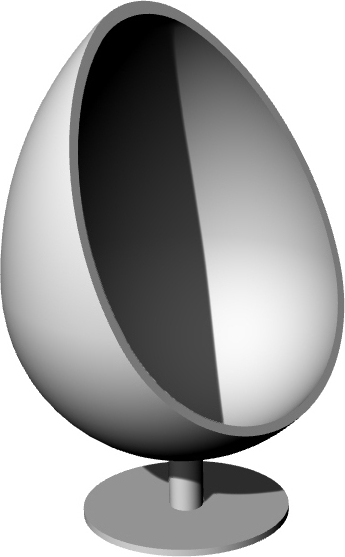
\includegraphics[height=4cm]{fig/case-study-egg-chair}}
  \hfill
  \subcaptionbox{Simple 4-leg chair.\label{fig:eval.studies.designs.thonet214}}
    [.2\linewidth]{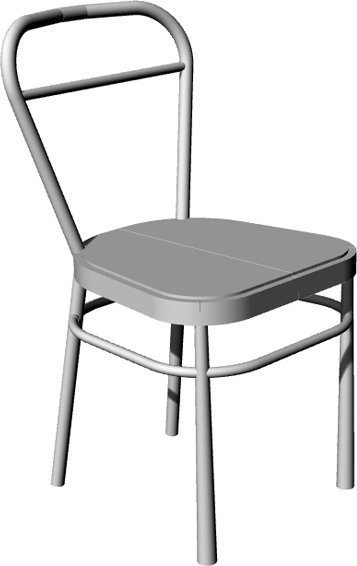
\includegraphics[height=4cm]{fig/case-study-thonet-214}}
  \hfill
  \subcaptionbox{Islamic towers.\label{fig:eval.studies.designs.petronas}}
    [.2\linewidth]{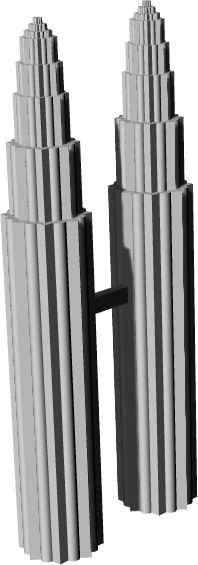
\includegraphics[height=4cm]{fig/case-study-petronas}}
  \hfill
  \subcaptionbox{Voronoi cage.\label{fig:eval.studies.designs.watercube}}
    [.35\linewidth]{%
      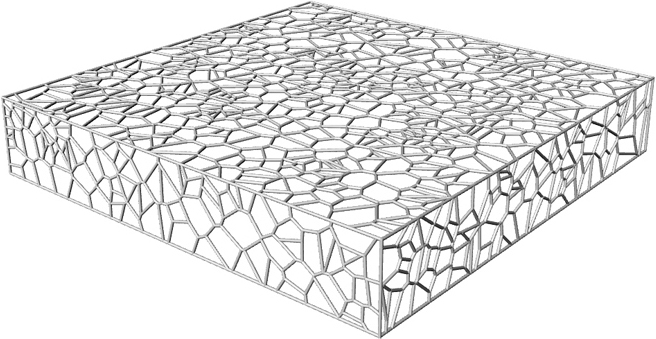
\includegraphics[width=\linewidth]{fig/case-study-water-cube}}
  \caption[Case study design inspirations]{
    Case study designs inspired by the Eero Aarnio's Egg
    chair~\subref{fig:eval.studies.designs.egg}, Thonet 214
    chair~\subref{fig:eval.studies.designs.thonet214},  César Pelli's Petronas
    Twin Towers~\subref{fig:eval.studies.designs.petronas}, and PTW Architects'
    Beijing National Aquatics
    Center~\subref{fig:eval.studies.designs.watercube}.}%
  \label{fig:eval.studies.designs}
\end{figure}

\subsection{Egg}%
\label{sec:eval.studies.egg}

The first case study is an egg shape (which can be considered a particular case
of an oval shape).  Examples of applications of this shape in design include the
Eero Aarnio's Egg chair, James Law's Cybertecture Egg building, and RAU
Architects and Ro\&Ad Architects' Tij observatory.

The egg shape is a broad concept, as it can refer to a wide range of curves
resembling an egg~\cite{Dixon:1991:Mathographics}.  In this case, our shape is
bilaterally symmetric and is composed of four arcs, the side arcs being tangent
to the bottom and top arcs.

Our parametrization of the egg defines four parameters: the bottom arc's center
$O_1$, the bottom and top arcs' radii $r_1$ and $r_2$ respectively, and the
egg's height $h$ (\cref{fig:eval.studies.egg.prob.params}).  Different egg
shapes, more or less elongated, can be obtained by varying the parameters'
values (\cref{fig:eval.studies.egg.prob.vars}).  One of those variations, where
$r_2 = (2 - \sqrt2)r_1$ and $h = 2r_1 + r_2$, corresponds to the Moss' Egg
(\cref{fig:eval.studies.egg.prob}, the egg with $h = 2.6$ and $r_2 = 0.6$).

\begin{figure}[htb]
  \subcaptionbox{\label{fig:eval.studies.egg.prob.params}%
    Egg parametrization: center $O_1$, bottom and top arcs' radii $r_1$ and
    $r_2$, and height $h$.}
    {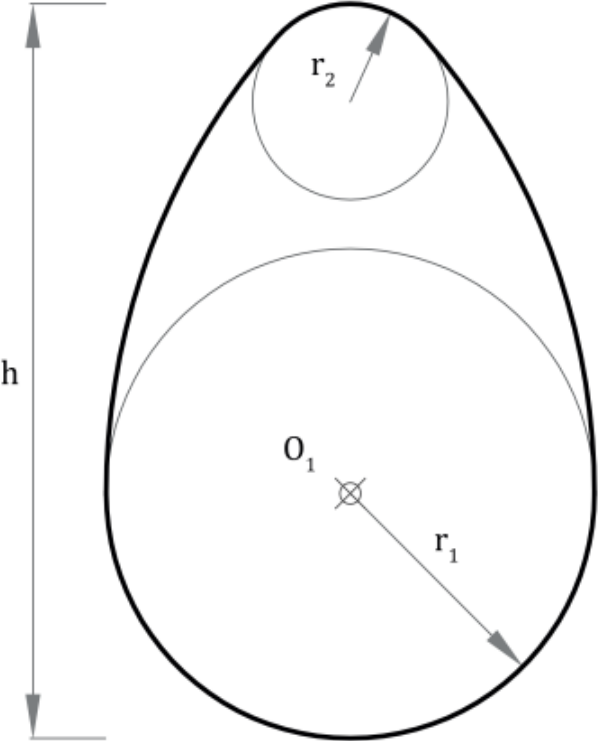
\includegraphics[height=7cm]{fig/egg-problem-params}}
  \hfill
  \subcaptionbox{\label{fig:eval.studies.egg.prob.vars}%
    Egg shape variations: variations change the values of the radius $r_3$ and
    the height $h$.}
    {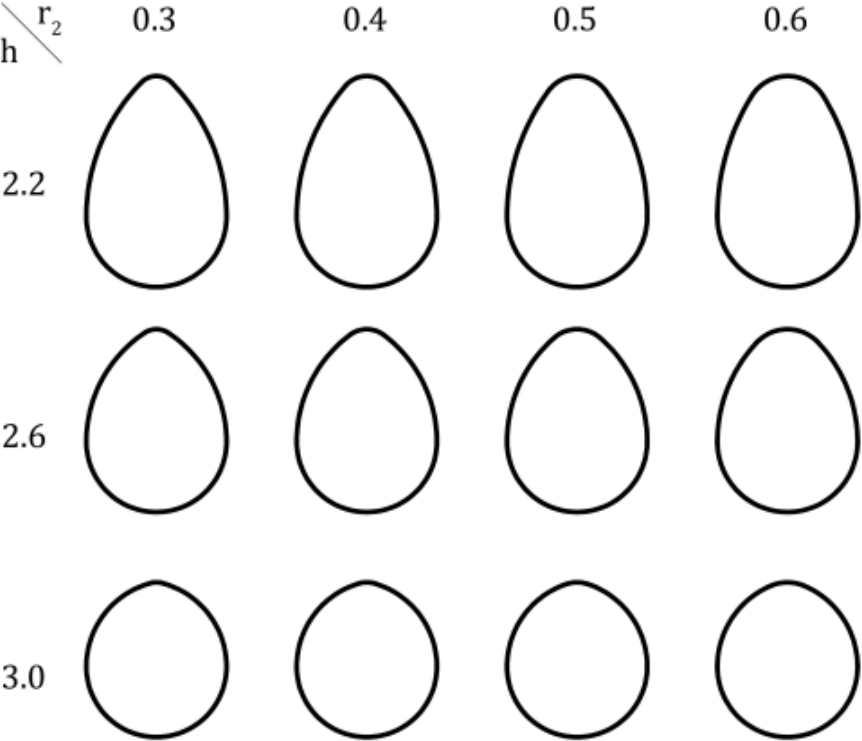
\includegraphics[height=7cm]{fig/egg-problem-vars}}
  \caption[Egg problem]{Egg problem:
  \subref{fig:eval.studies.egg.prob.params} shows our parametrization of the
  egg which can be used to generate shape variations, some of them shown in
  \subref{fig:eval.studies.egg.prob.vars}.}\label{fig:eval.studies.egg.prob}
\end{figure}

In this case, the major problem was to define the side arc $A_3$, which is given
by the center $O_3$, radius $r_3$, and amplitude $\alpha$
(\cref{fig:eval.studies.egg.sol.a}). The \textit{analytic solution} is described
below. The angle $\alpha$ and the radius $r_3$ are devised from the triangle
$\triangle O_1 O_2 O_3$ (\cref{fig:eval.studies.egg.sol.c}), and the center
$O_3$ is given by a translation of $O_1$ through the unit vector $\vec{e}_x$,
parallel to the X-axis, scaled by the factor $r_1 - r_3$.  It is important to
note that, despite their simplicity, the derivations needed to arrive at the
following formulas are not obvious.

\begin{enumerate}
  \item $\alpha = 2\arctan\frac{r_1 - r_2}{h - r_1 - r_2}$
  \item $r_3 = \frac{r_1 - r_2 \cos\alpha}{1 - \cos\alpha}$
  \item $O_3 = O_1 + \left(r_1 - r_2\right)\vec{e}_x$
\end{enumerate}

The \textit{constructive solution} is based on the geometric problem of
determining the \textit{tangent line to two circles}.  In fact, the side arc
$A_3$ is tangent to two circles, $C_1$ and $C_2$, and passes through point
$P_1$.  Two \ac{GC} primitives from our solution were employed in this
solution, namely \textit{intersection} and \textit{bisector}.  The solution can
be computed according to the following procedure
(\cref{fig:eval.studies.egg.sol.c}):

\begin{enumerate}
  \item $C_{2}' = \mathrm{circle}\left(P_1, r_2\right)$%
  \label{enum:eval.studies.egg.cs}
  \item $I = \mathrm{intersection}\left(C_{2}', \overline{O_1 P_2}\right)$
  \item $B = \mathrm{bisector}\left(\overline{IO_2}\right)$
  \item $O_3 = \mathrm{intersection}\left(B, O_1 P_1\right)$
  \item $r_3 = \mathrm{length}\left(\overline{O_3 P_1}\right)$%
  \label{enum:eval.studies.egg.ce}
  \item $\alpha = \mathrm{angle}\left(O_2,O_3,O_1\right)$
\end{enumerate}

We can further increase the expressive level of the solution by defining the
$\mathrm{tangent_{circle}}$ functionality.  Given two circles, $C_1$ and $C_2$,
and a point $P_1$ on $C_1$, $\mathrm{tangent_{circle}}$ produces the circle
tangent to both $C_1$ and $C_2$ that goes through $P_1$.  This way, the solution
can be simplified by replacing steps \ref{enum:eval.studies.egg.cs} through
\ref{enum:eval.studies.egg.ce} by using the $\mathrm{tangent_{circle}}$
functionality as follows:

\begin{enumerate}
  \item $O_3,r_3 = \mathrm{tangent_{circles}}\left(C_1, C_2, P_2\right)$
  \item $\alpha = \mathrm{angle}\left(O_2, O_3, O_1\right)$
\end{enumerate}

In the egg's case, $C_1$ must be larger than $C_2$, and $P_1$ is one of the
intersection points between the horizontal line that passes through $O_1$ and
the circle $C_1$.

\begin{figure}[htb]
  \subcaptionbox{\label{fig:eval.studies.egg.sol.a}%
      Solution using the analytic approach.}
    {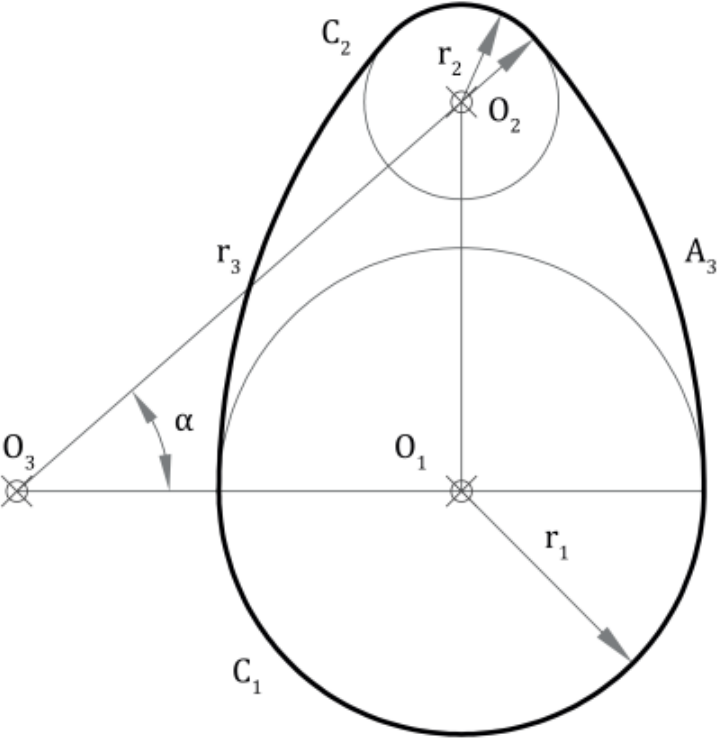
\includegraphics[height=7cm]{fig/egg-solution-analytic}}
  \hspace{\fill}
  \subcaptionbox{\label{fig:eval.studies.egg.sol.c}%
      Solution using the constructive approach.}
    {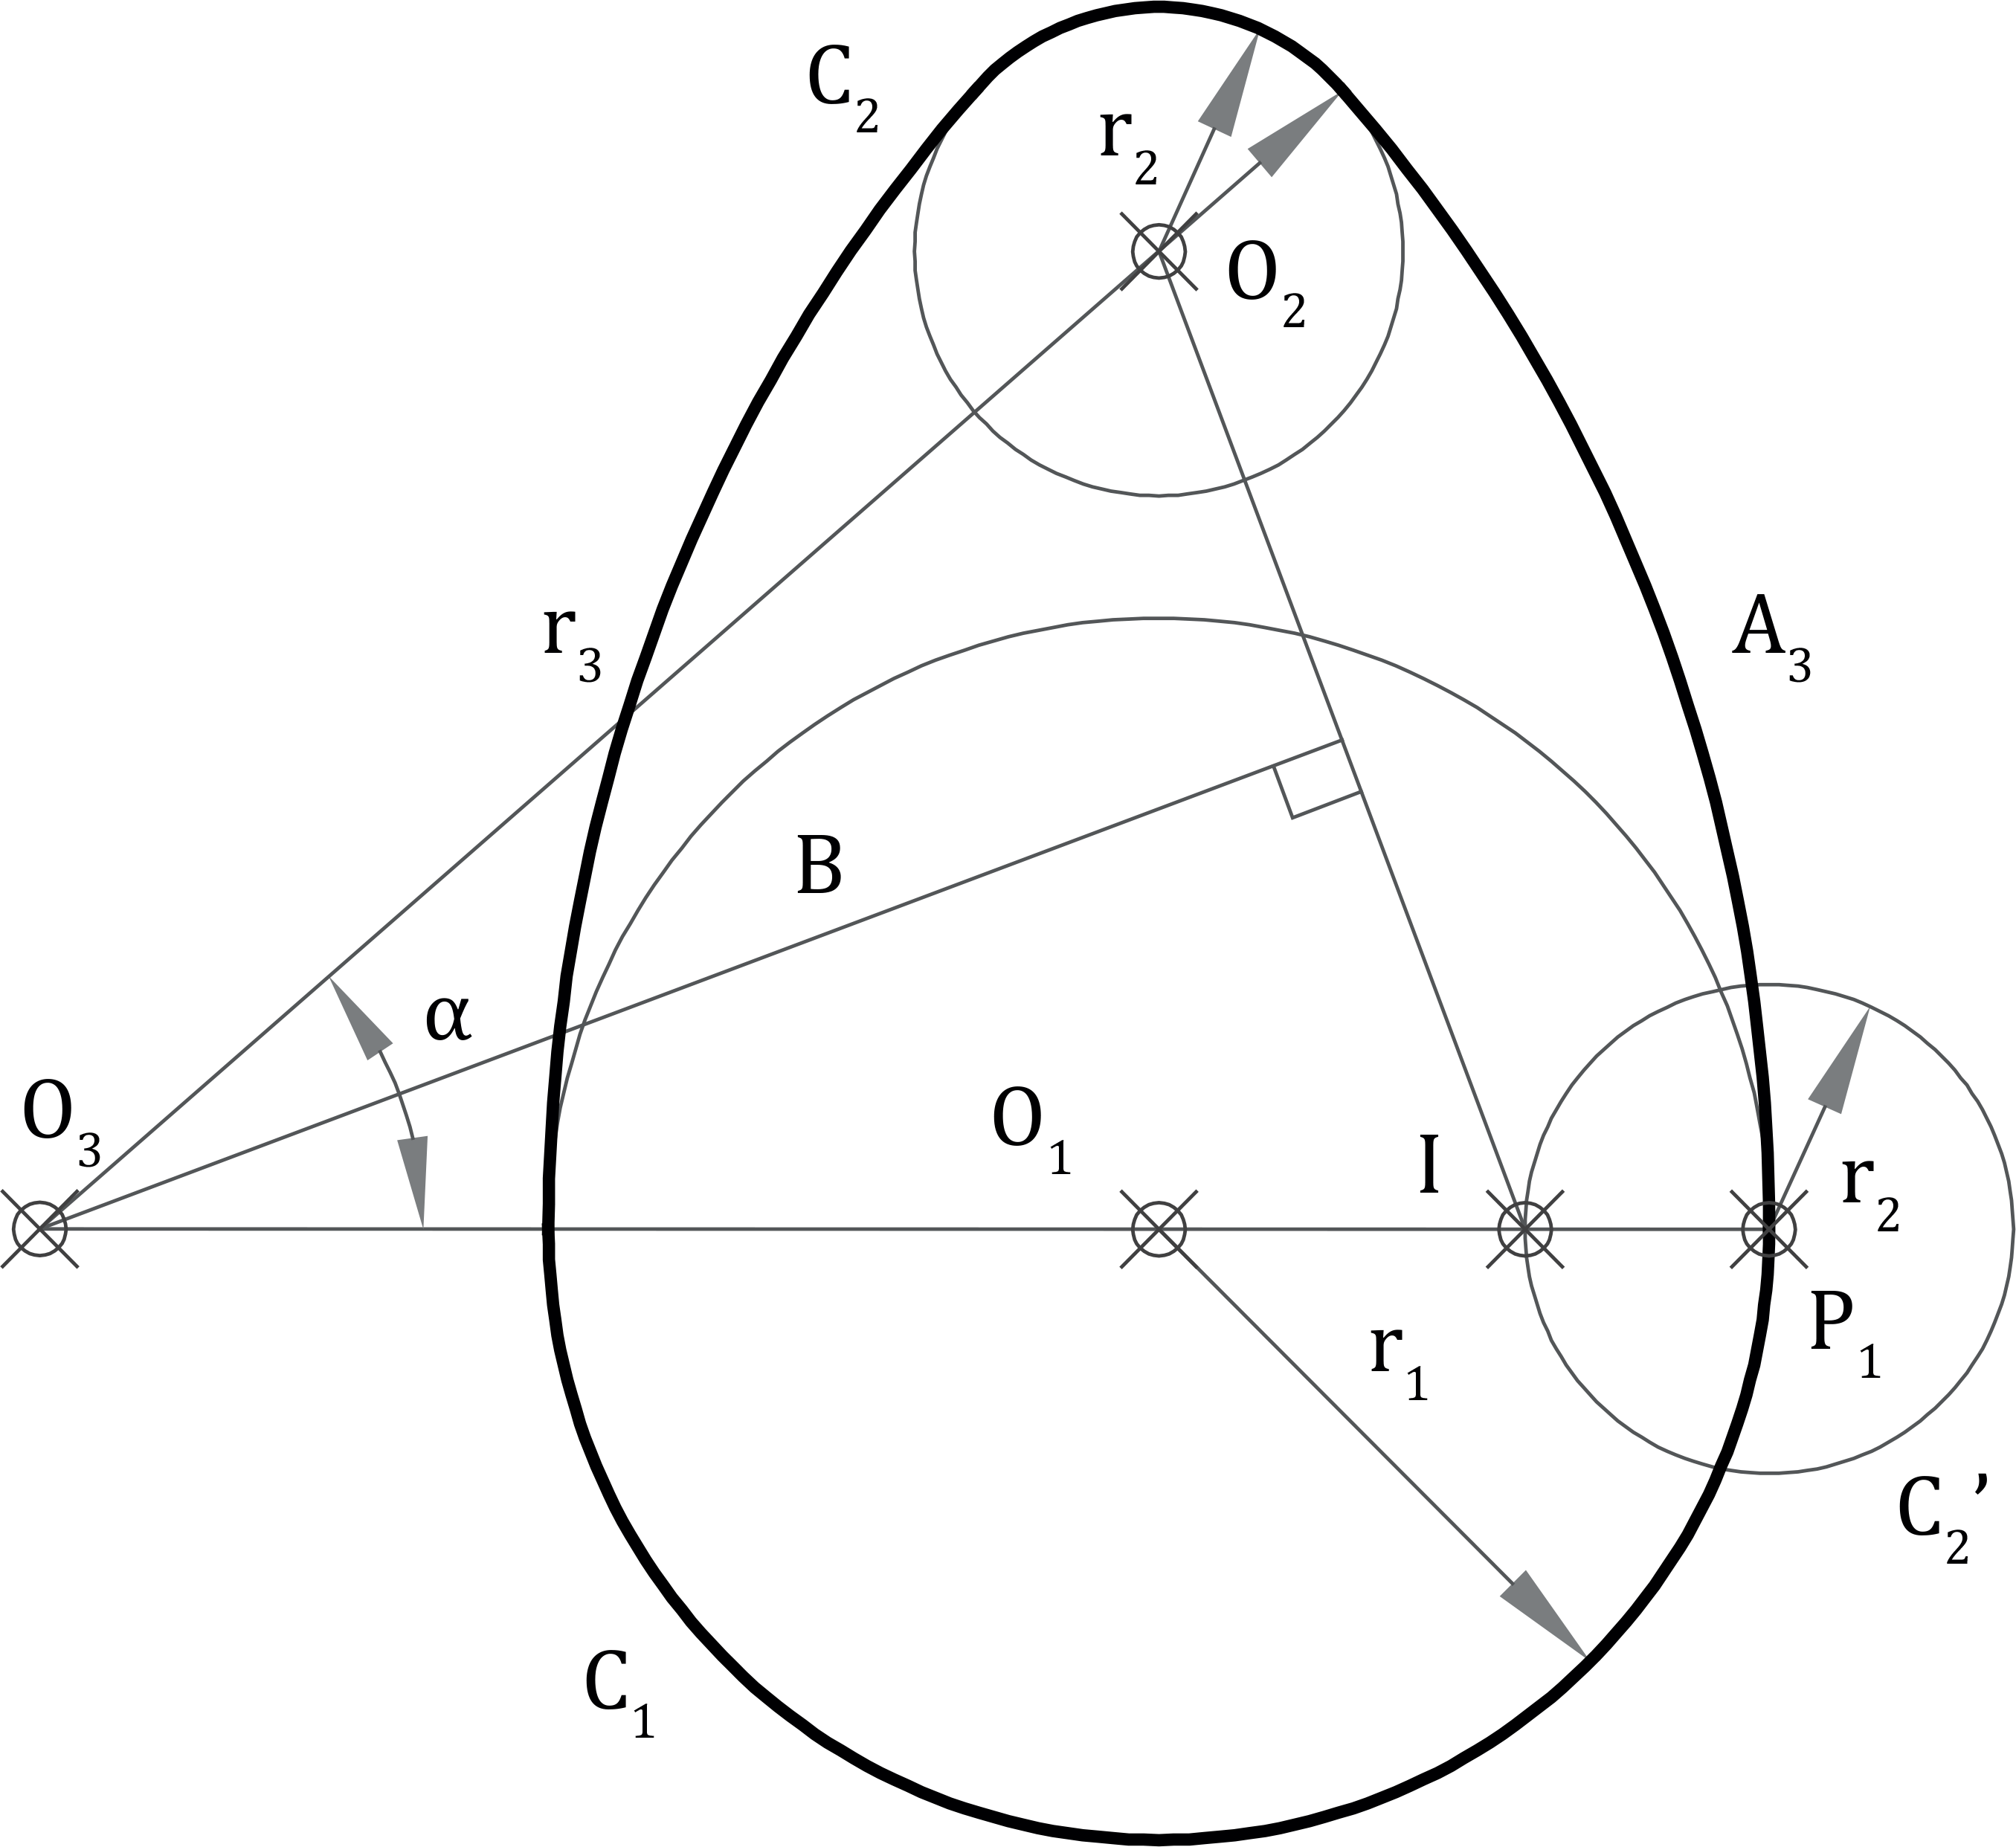
\includegraphics[height=7cm]{fig/egg-solution-constructive}}
  \caption[Egg problem solutions]{Solutions to the Egg problem using two
    different approaches.}%
  \label{fig:eval.studies.egg.sol}
\end{figure}

Achieving the equations in the \textit{analytic solution} is not a
straightforward task for designers, since it involves considerable logical
reasoning and the use of non-trivial formulas (such as trigonometric half-angle
identities). It is also unclear how those equations were derived. By contrast,
in the \textit{constructive solution}, all the steps are clearly externalized,
which makes it much more comprehensible.

\subsection{Rounded Trapezoid}%
\label{sec:eval.studies.rtrapezoid}

The second case study is a rounded trapezoid shape.  This parametric shapes is
used in the contour of a variety of different chair seats, such as the Thonet
214 and the Zig Zag chairs~\cite{Garcia:2018:SGDTIMCG}.  This shape is
bilaterally symmetric and is defined by six parameters: width $w$, depth $d$,
taper width $tw$, front radius $r_f$, rear radius $r_r$, and origin $O$
(\cref{fig:eval.studies.rtrapezoid.prob.params}).  The taper width and front and
rear radii are ratios of the width and the depth.  By varying these parameters'
values, one can obtain different shapes, such as a square, a trapezoid, a
triangle, a rounded rectangle, a drop-like shape, and a circle, among others
(\cref{fig:eval.studies.rtrapezoid.prob.vars}).

\begin{figure}[htb]
  \subcaptionbox{\label{fig:eval.studies.rtrapezoid.prob.params}%
    Trapezoid parametrization: width $w$, depth $d$, taper width $w$, front and
    rear radii $r_f$ and $r_r$ respectively, and origin $O$.}
    {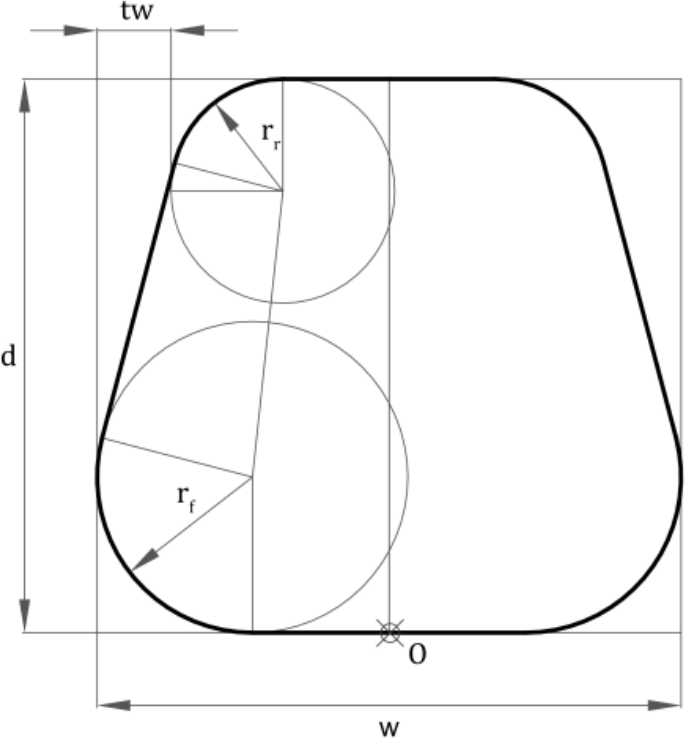
\includegraphics[height=7cm]{fig/rtrapezoid-problem-params}}
  \hfill
  \subcaptionbox{\label{fig:eval.studies.rtrapezoid.prob.vars}%
    Rounded trapezoid shape variations: variations change the values of the
    front radius $r_f$ and the taper width $tw$.}
    {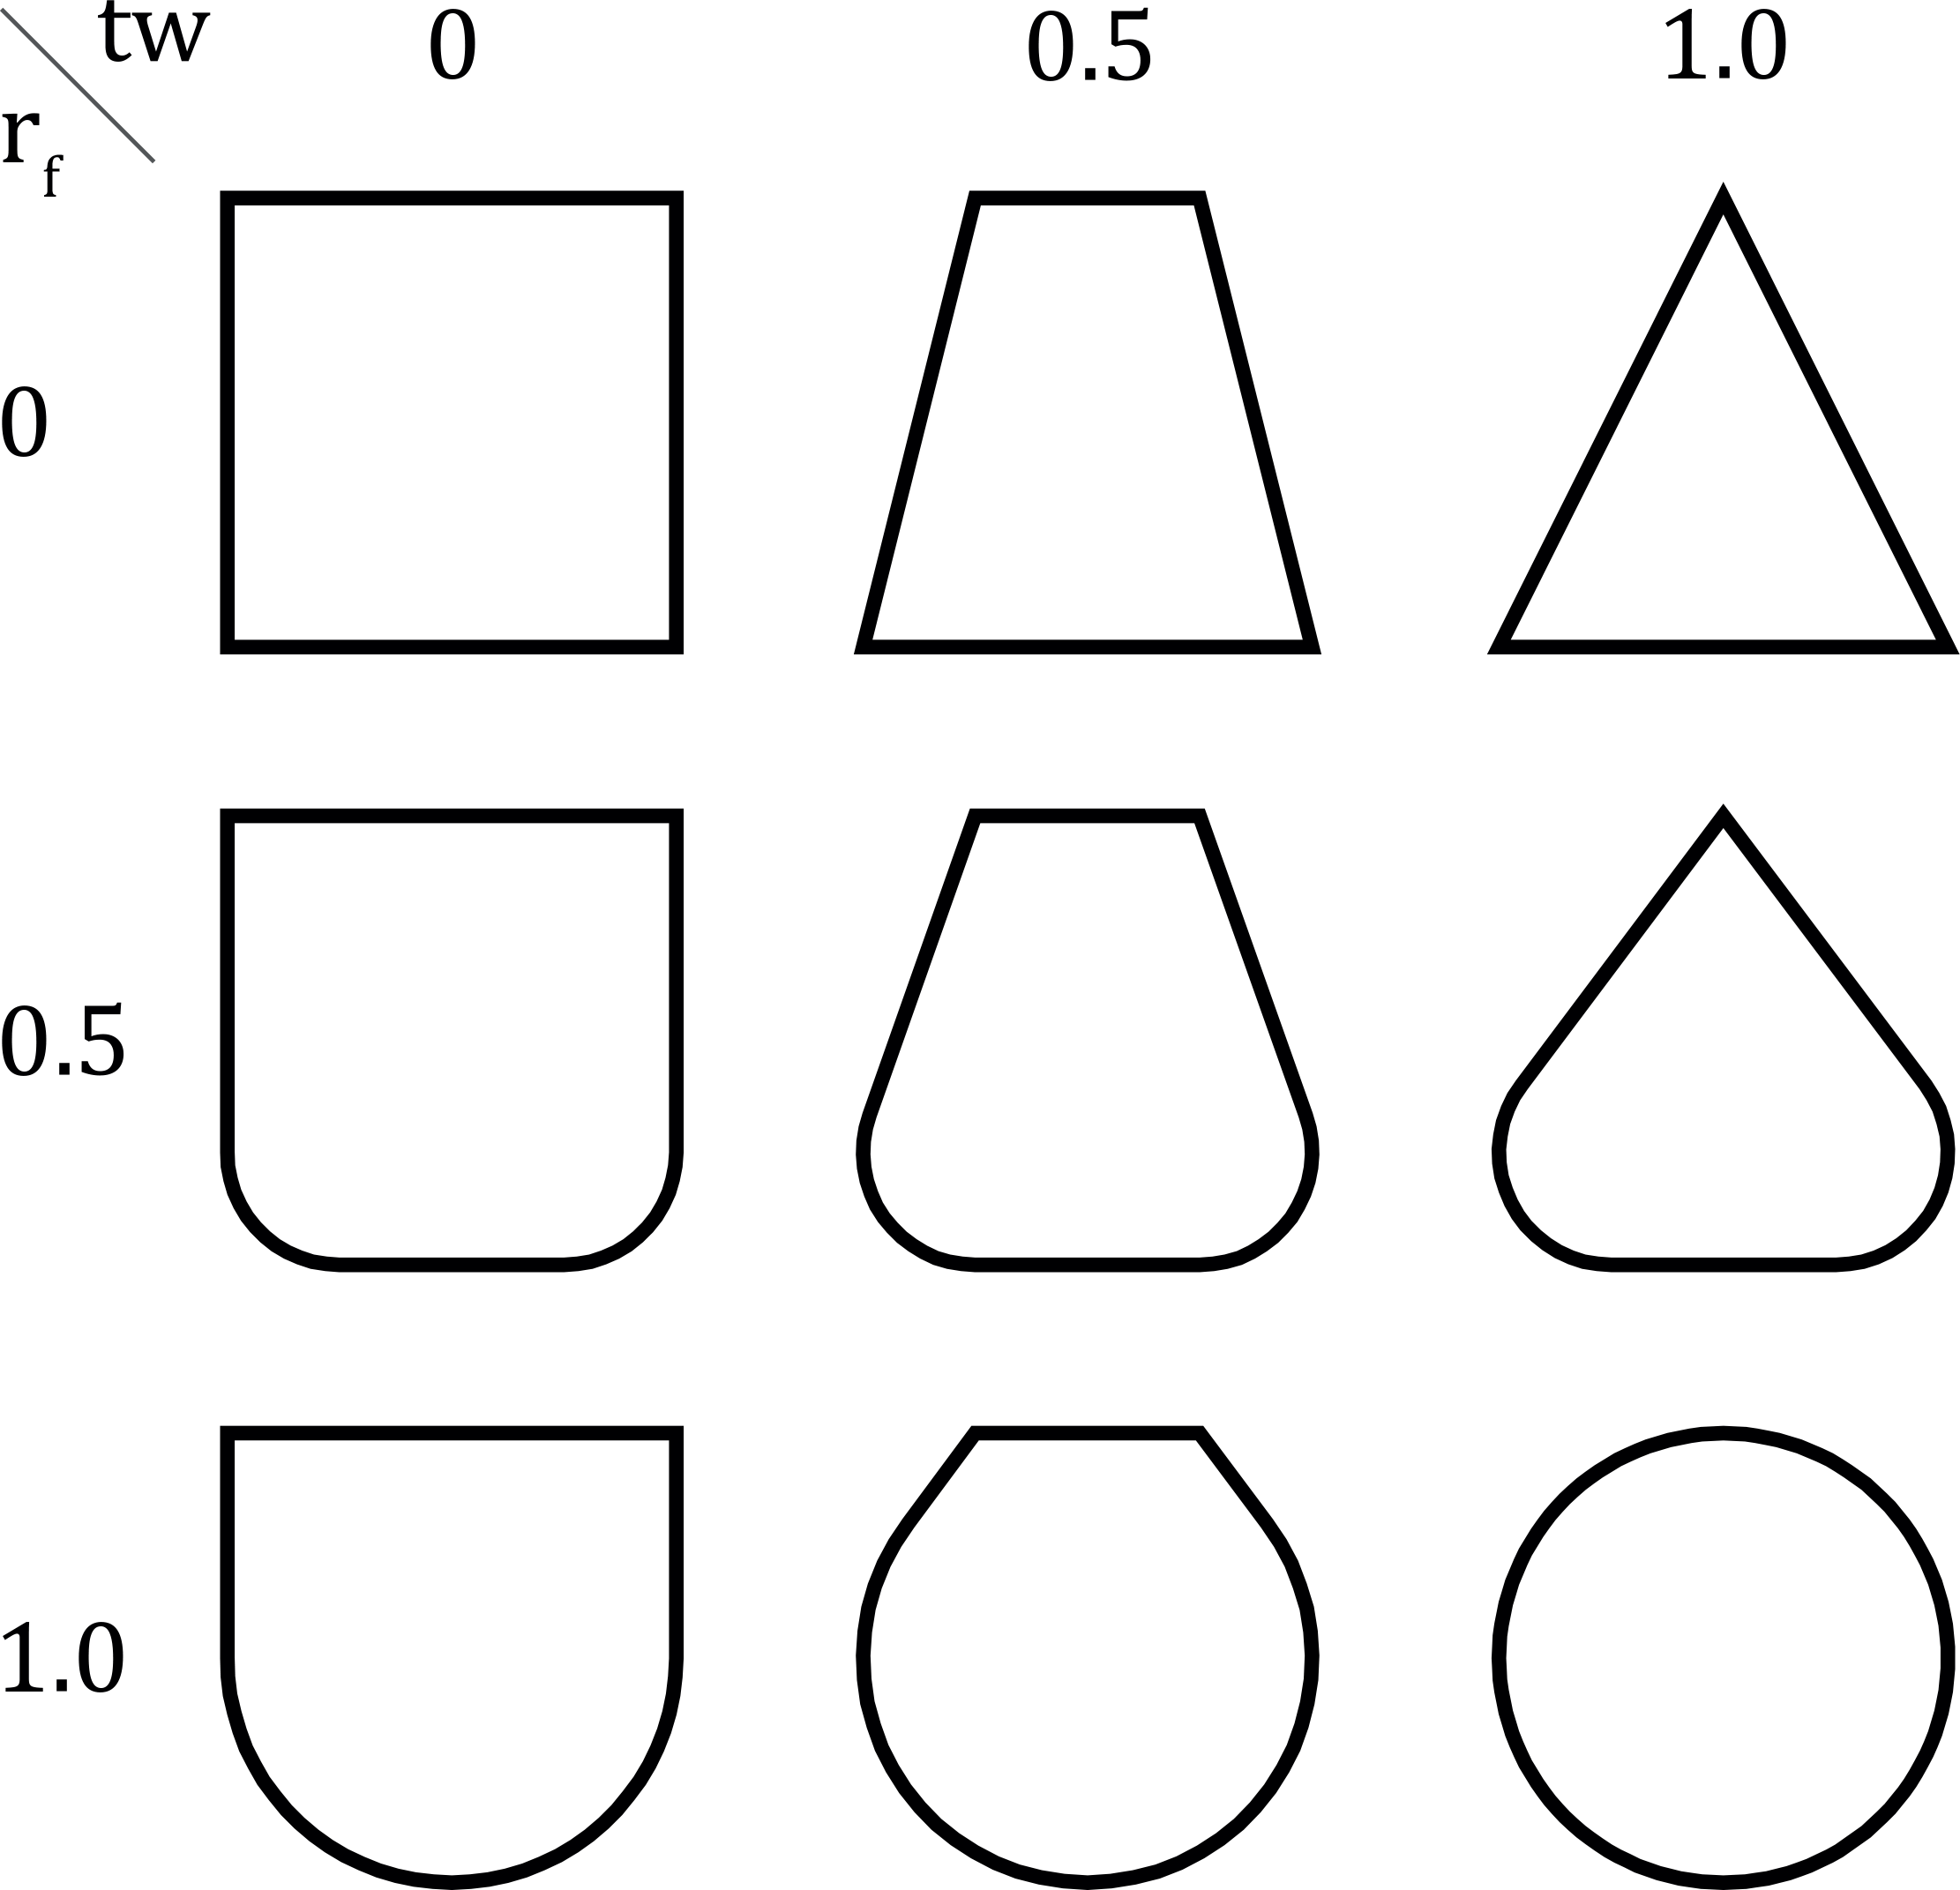
\includegraphics[height=7cm]{fig/rtrapezoid-problem-vars}}
  \caption[Rounded trapezoid problem]{Rounded trapezoid problem:
    \subref{fig:eval.studies.rtrapezoid.prob.params} shows our parametrization
    of the trapezoid which can be used to generate shape variations, some of
    them shown in \subref{fig:eval.studies.rtrapezoid.prob.vars}.}%
  \label{fig:eval.studies.rtrapezoid.prob}
\end{figure}

One side of the chair is obtained by two circles and the \textit{tangent line to
two circles}, while the other side is a reflection of the former side.  Given
two circles $C_2$ and $C_2$, centered on $O_1$ and $O_2$ with radii $r_1$ and
$r_2$ respectively (\cref{fig:eval.studies.rtrapezoid.sol}), two solutions can
be delineated that can accurately reproduce the tangent line $\overline{T_1
T_2}$.

The \textit{analytic solution} is achieved by calculating the angle $\delta$
between the line segment $\overline{O_1 O_2}$ and the line perpendicular to the
tangent line between the two circles passing through $O_1$.  The angle $\theta$
is given by the slope of $\overline{O_1 O_2}$.  The point $T_1$ is given by a
translation of $O_1$ through a vector $\left(r_1, \angle\delta + \theta\right)$
where $r_1$ is its length and $\angle\delta + \theta$ is its polar angle.  A
similar approach is used to obtain $T_2$.

\begin{enumerate}
  \item $\delta = \arccos\frac{r_1 - r_2}{\lVert O_2 - O_1 \rVert}$
  \item $\theta = \angle\vv{O_2 - O_1},\vec{e}_x$
  \item $T_2 = O_1 + \left(r_1, \angle\delta + \theta\right)$
  \item $T_2 = O_2 + \left(r_1, \angle\delta + \theta\right)$
\end{enumerate}

The \textit{constructive solution} follows a sequence of steps that reflects the
geometric characteristics of the problem
(\cref{fig:eval.studies.rtrapezoid.sol}).  Four \ac{GC} primitives were employed
in this solution, namely \textit{midpoint}, \textit{intersection}, and
\textit{parallel lines}.

\begin{figure}
  \centering
  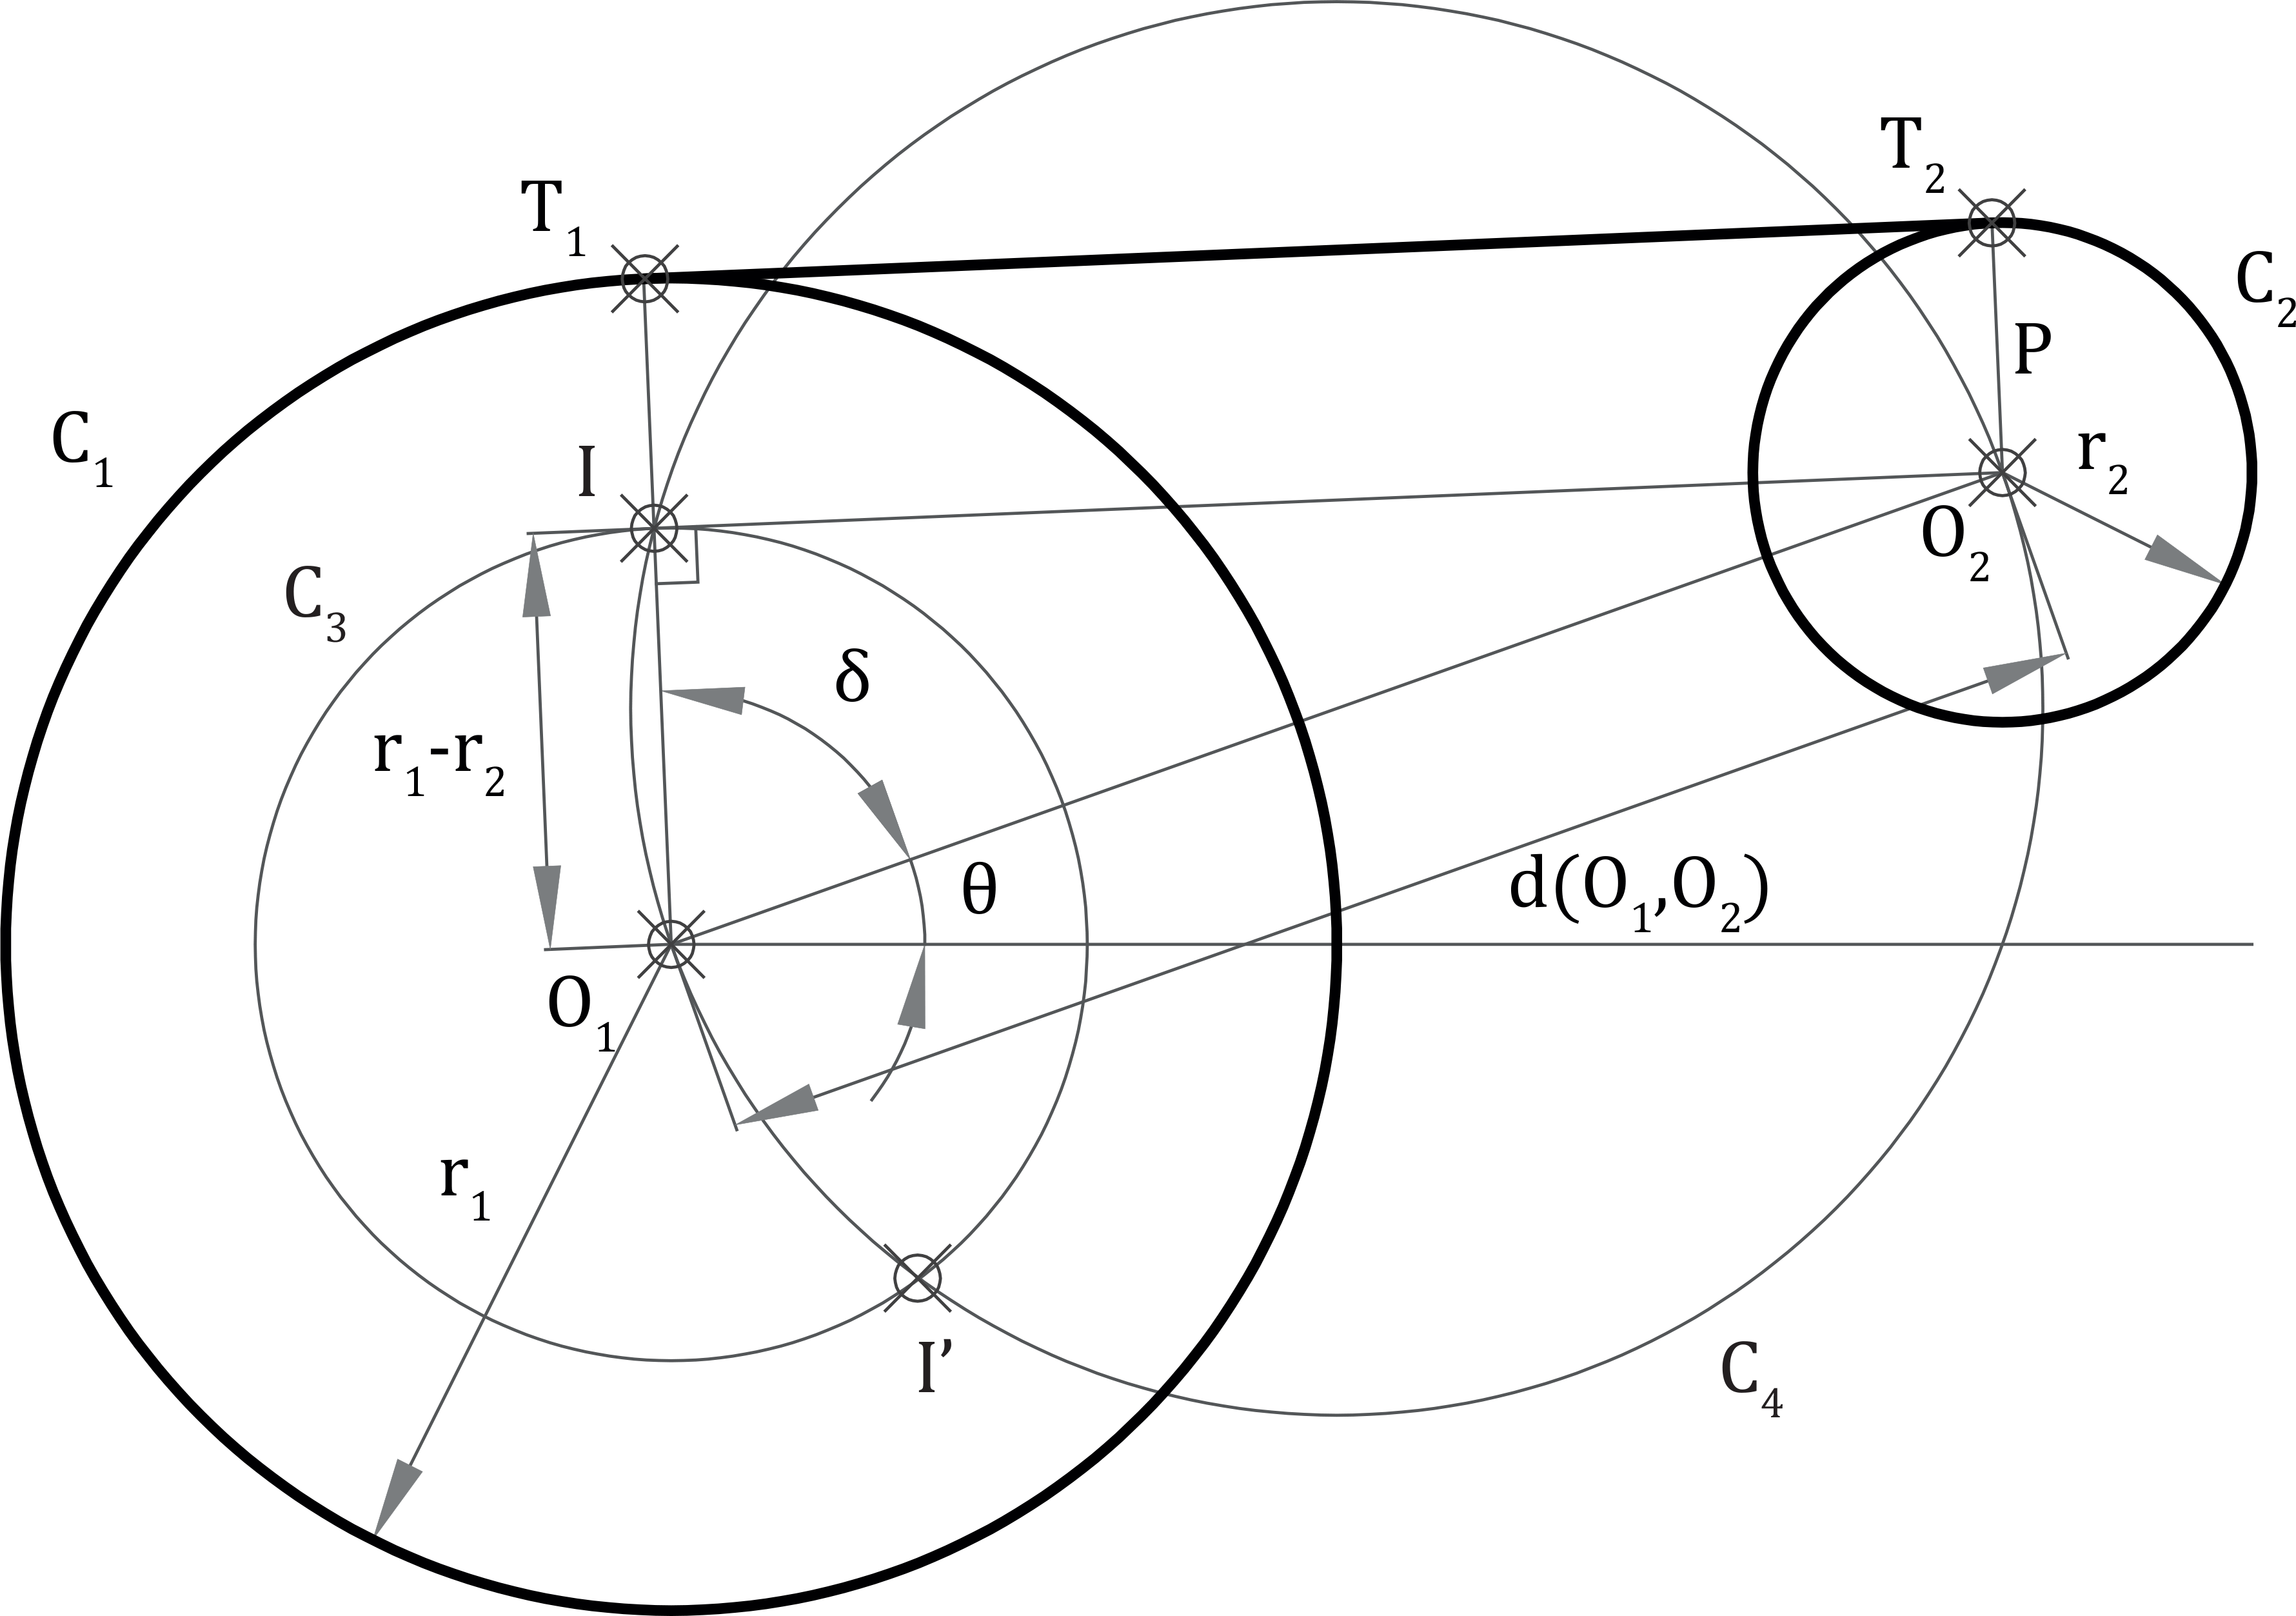
\includegraphics[height=7cm]{fig/rtrapezoid-solution}
  \caption[Rounded trapezoid problem solution]{Both analytic and constructive
    solutions to the rounded trapezoid problem.}%
  \label{fig:eval.studies.rtrapezoid.sol}
\end{figure}

\begin{enumerate}
  \item $C_3 = \mathrm{circle}\left(O_1, r_1 - r_2\right)$
  \item $M = \mathrm{midpoint}\left(O_1, O_2\right)$
  \item $d = \mathrm{length}\left(\overline{O_1 O_2}\right)$
  \item $C_4 = \mathrm{circle}\left(M, \frac{d}{2}\right)$
  \item $I,I' = \mathrm{intersection}\left(C_3, C_4\right)$
  \item $P = \mathrm{parallel}\left(\overline{IO_1, O_2}\right)$
  \item $T_1 = \mathrm{intersection}\left(IO_1, C_1\right)$
  \item $T_2 = \mathrm{intersection}\left(P, C_2\right)$
\end{enumerate}

Despite the adequacy of the \textit{analytic solution} for the design problem at
hand, it only produces the external tangent needed to solve this specific
problem, which works well if the circle's center is on the 1\textsuperscript{st}
and 2\textsuperscript{nd} quadrants: however, in the remaining quadrants, it
produces an unintended tangent.  In contrast, our \textit{constructive approach}
is capable of producing a solution independently of how the circles are
arranged.

The advantage of using well-established functions from \ac{CGAL} is that they
deal with degenerate cases better than re-implementations of the same
functionality from scratch.  For instance, in the case of concentric circles,
the intersection between those circles does not produce an error; instead, it
produces an empty result.  In the case of the proposed \textit{analytic
solution}, the distance between the circles' centers is zero, which leads to a
division-by-zero error.

Architects and designers are used to manipulating \acp{GC}, such as
\textit{tangency}, \textit{parallelism}, and \textit{intersection}, and less
inclined to deal with the mathematical intricacies of analytic geometry, which
makes the second approach more appealing to them.  To that end, we can introduce
the $\mathrm{tangent_{lines}}$ functionality, which, given two circles $C_1$ and
$C_2$, produces a sequence of tangent lines between the circles, allowing the
user to select the lines that best suit the problem.  This allows us to reduce
the solution to the single step
\begin{itemize}
  \item[] $\overline{T_1 T_2},\ldots = \mathrm{tangent_{lines}}\left(C_1,
  C_2\right)$
\end{itemize}
where $\overline{T_1 T_2}$ is one of the lines of the sequence.

Depending on how the circles are arranged, there can be multiple solutions:
\begin{enumerate*}[label= (\arabic*)]
  \item no segments, if one circle contains the other,
  \item two segments, if the circles intersect, or
  \item four segments, if the circles are disjoint.
\end{enumerate*}
The advantage of having the $\mathrm{tangent_{lines}}$ functionality is that it
is capable of finding every solution to the generic \textit{tangent line to two
circles} problem.  Hence, the user can reutilize this functionality each time
a different problem of a similar nature arises.

\subsection{Star with Semicircles}%
\label{sec:eval.studies.star}

The third case study is a star shape with semicircles.  This shape was inspired
by César Pelli's Petronas tower floor plan, which in turn mimics Islamic
patterns.  The contour of the Petronas tower floor plan is formed by two
overlapping congruent squares, forming an octagram known as Star of Lakshmi, and
by eight circles centered on each of the eight intersection points and tangent
to the bounding octagon.  This shape can be generalized to a parametric shape
defined by three parameters: origin $O$, radius $r$, and number of vertices $n$
(\cref{fig:eval.studies.star.prob.params}).  Note that the number of vertices
cannot be less than five.  Five variations, comprising stars with 5 to 9
vertices, are illustrated in \cref{fig:eval.studies.star.prob}.

\begin{figure}[htb]
  \centering
  \subcaptionbox{\label{fig:eval.studies.star.prob.params}%
    Star parametrization: origin $O$, radius $r$, and number of vertices $n$.}
    {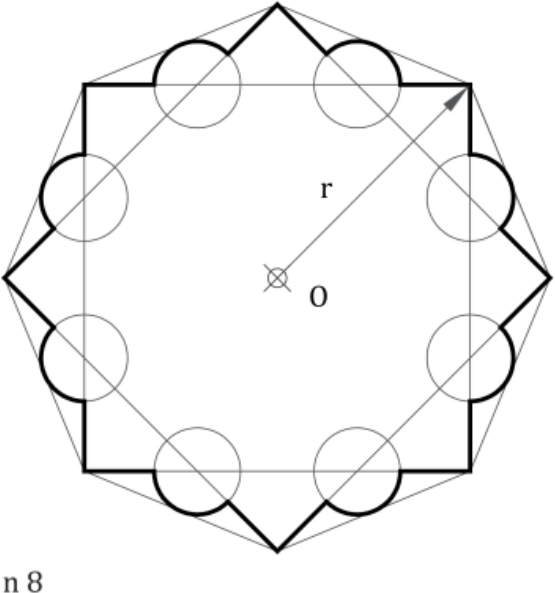
\includegraphics[height=7cm]{fig/star-problem-params}}
  \hfill
  \subcaptionbox{\label{fig:eval.studies.star.prob.vars}%
    Star shape variations: variations change the values of the number of
    vertices $n$.}
    {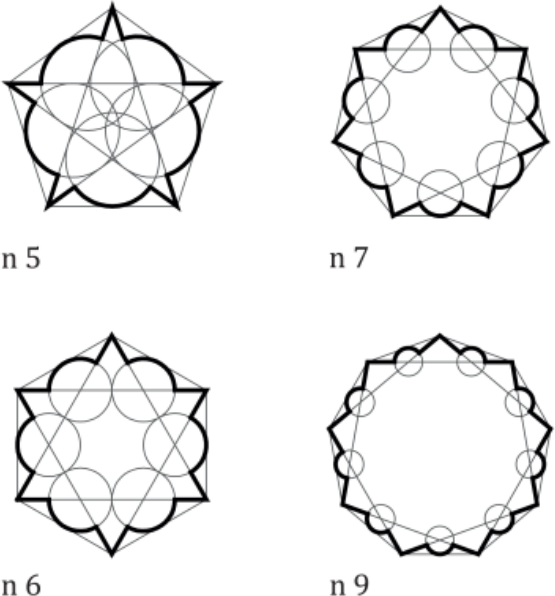
\includegraphics[height=7cm]{fig/star-problem-vars}}
  \caption[Star with semicircles problem]{Star with semicircles problem:
    \subref{fig:eval.studies.star.prob.params} shows our parametrization of
    the star which can be used to generate shape variations, some of them
    shown in \subref{fig:eval.studies.star.prob.vars}.}%
  \label{fig:eval.studies.star.prob}
\end{figure}

Both analytic and constructive solutions are based on computing one side of the
star, composed of the line segment $\overline{V_1 I_1}$, the arc centered on
$O_1$ from $I_1$ to $I_2$, with radius $r_1$, and the line segment 
$\overline{I_2 V_2}$ (\cref{fig:eval.studies.star.sol}).  The remaining sides
result from the recursive application of the preceding side with a rotation
transformation around the center.

\begin{figure}[htb]
  \centering
  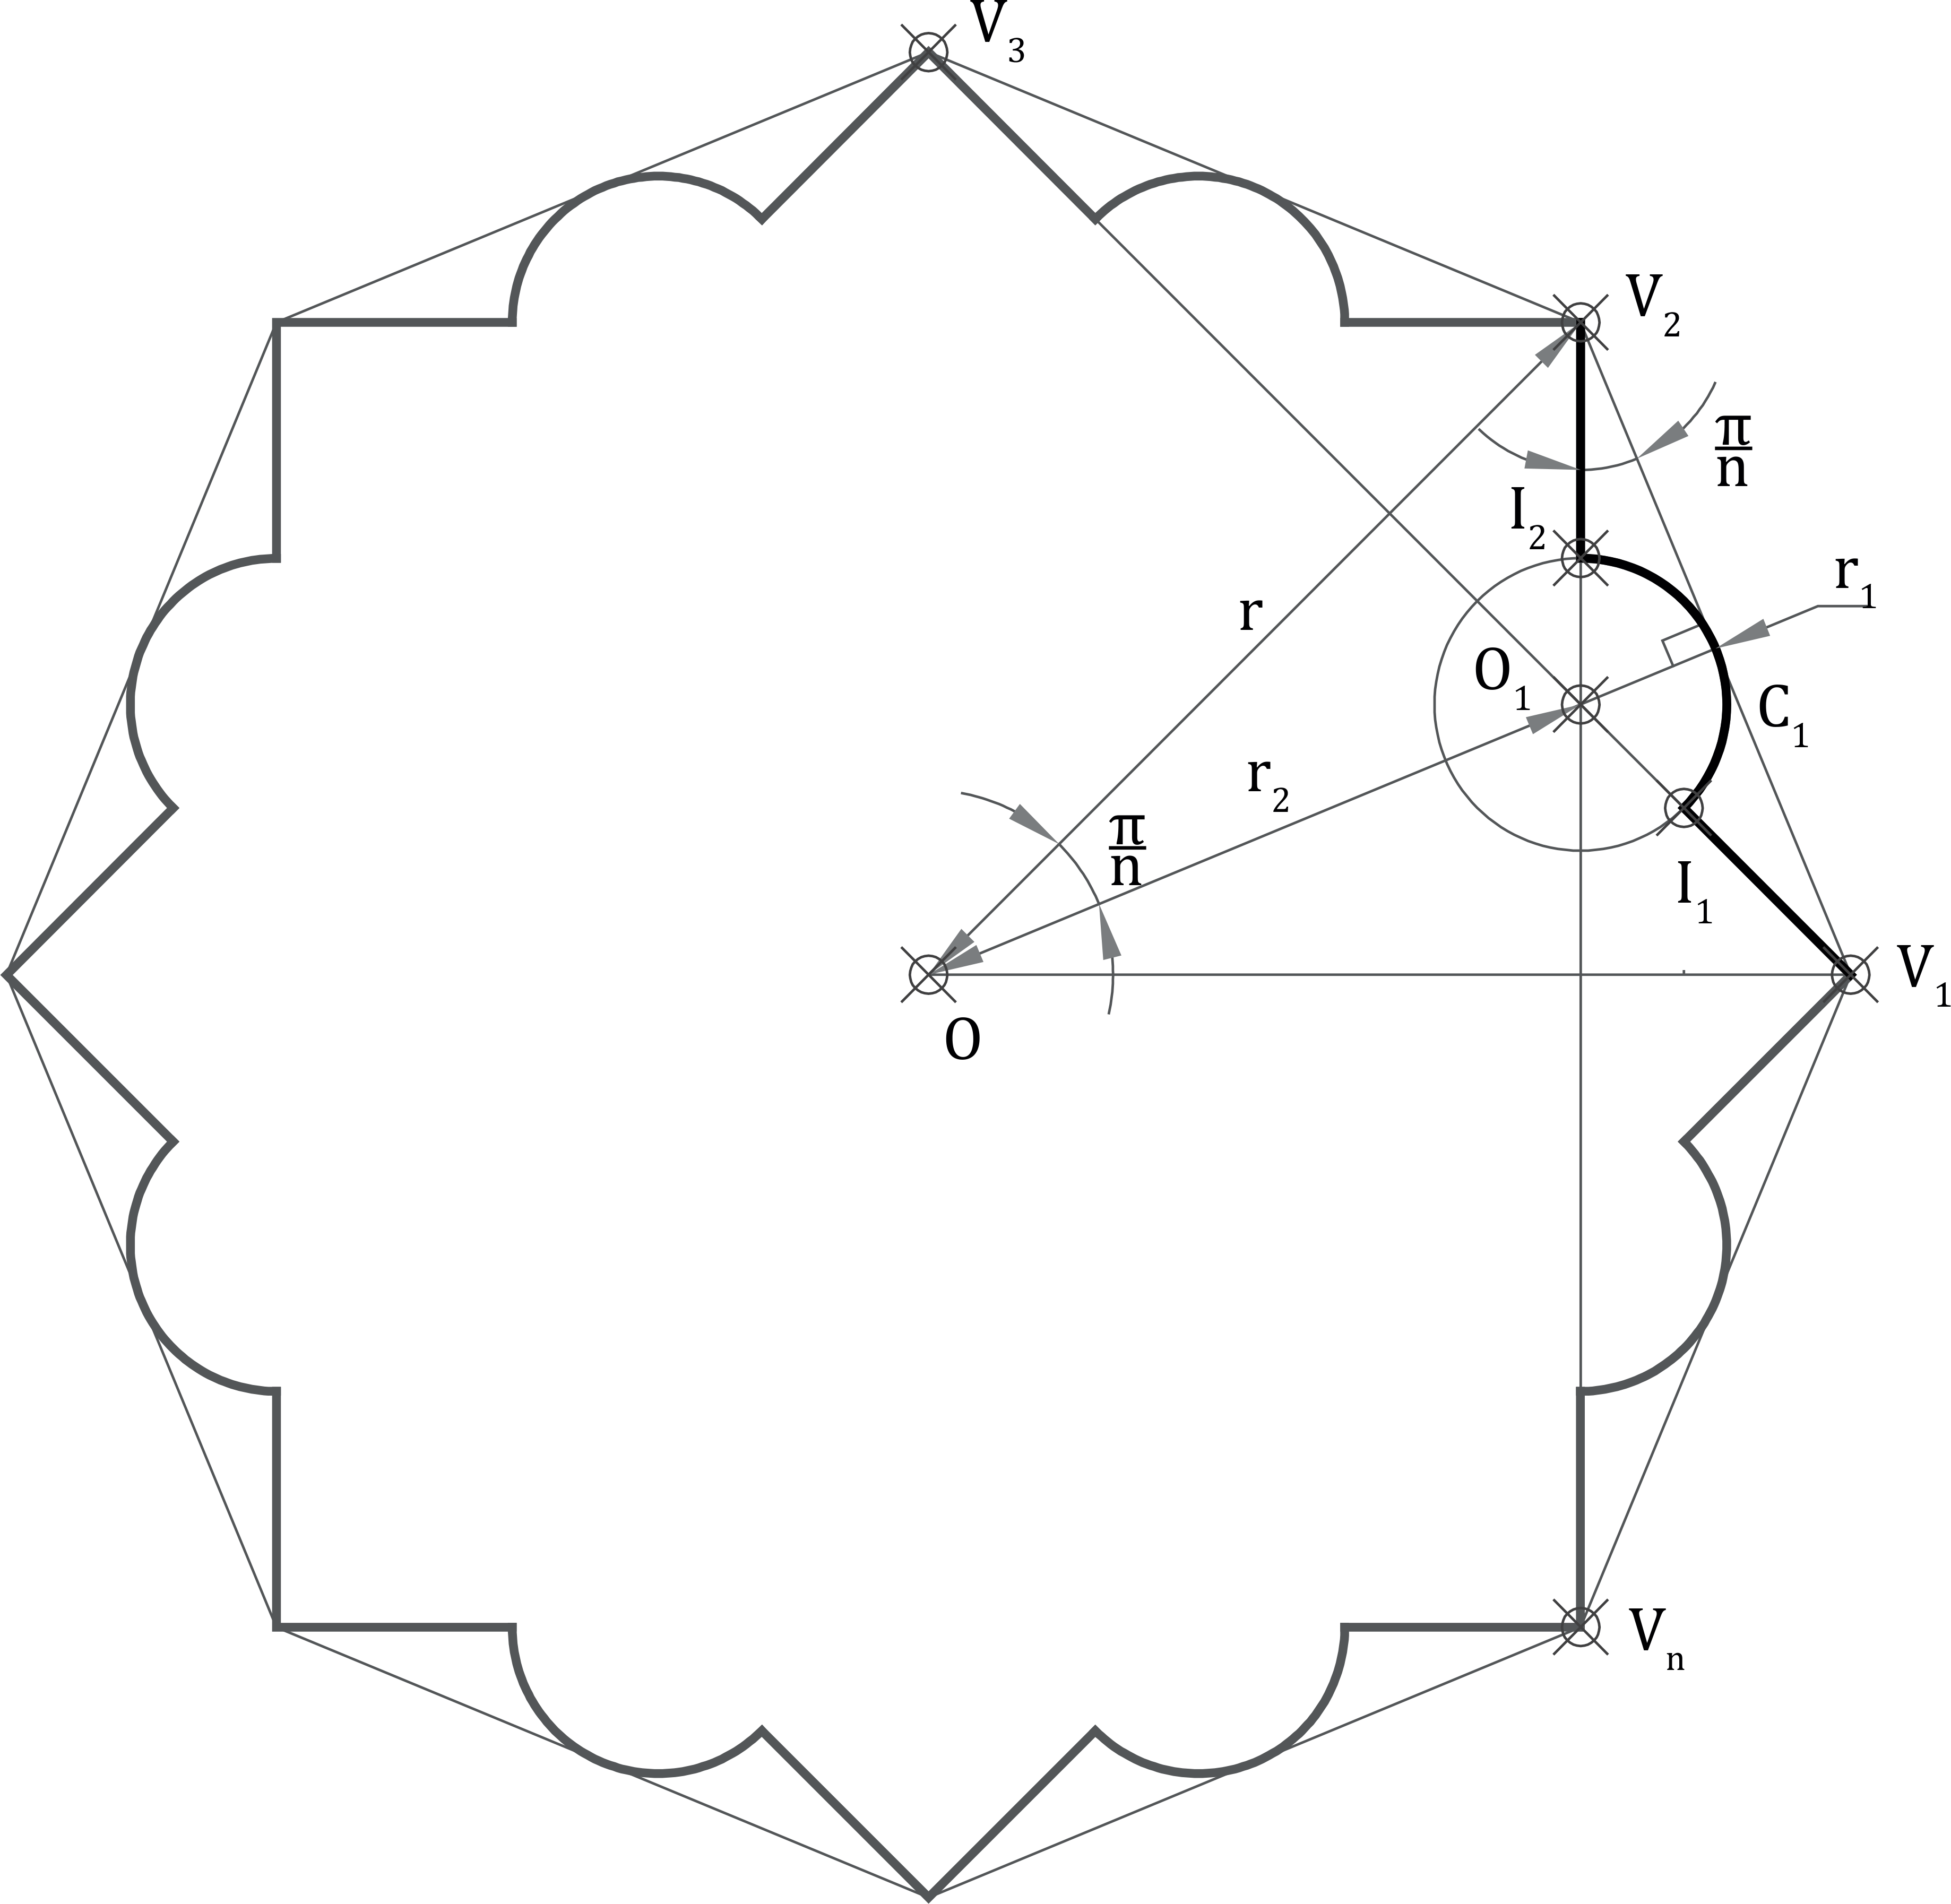
\includegraphics[height=9cm]{fig/star-solution}
  \caption[Star with semicircles problem solution]{ Both analytic and
    construction solutions to the star with semicircles problem.}%
  \label{fig:eval.studies.star.sol}
\end{figure}

The \textit{analytic solution} is described below.  The radius $r_1$ of the
circle $C_1$ is calculated by step \ref{enum:eval.studies.star.r1}, the radius
$r_2$ is defined by step \ref{enum:eval.studies.star.r2}, and its center $O_1$
is given by step \ref{enum:eval.studies.star.O1}.  The intersection points $I_1$
and $I_2$ are given by a rotation around $O_1$
(\cref{fig:eval.studies.star.sol}).

\begin{enumerate}
  \item $r_1 = r\frac{\sin^2\frac{\pi}{n}}{\cos\frac{\pi}{n}}$%
  \label{enum:eval.studies.star.r1}
  \item $r_2 = r\cos\frac{\pi}{n} - r_1$%
  \label{enum:eval.studies.star.r2}
  \item $O_1 = O + \left(r_2, \angle\frac{\pi}{n}\right)$%
  \label{enum:eval.studies.star.O1}
  \item $I_1 = O_1 + \left(r_1, \angle\frac{2\pi}{n} - \frac{\pi}{2}\right)$
  \item $I_2 = O_1 + \left(r_1, \angle\frac{\pi}{2}\right)$
\end{enumerate}

The \textit{construction solution} is based on finding the position and size of
the circle $C_1$ (see \cref{fig:eval.studies.star.sol}).  Two \ac{GC}
primitives were employed in this solution, namely \textit{intersection}, and
\textit{tangent circle to one line}.

\begin{enumerate}
  \item $O_1 = \mathrm{intersection}\left(\overline{V_1 V_3}, \overline{V_2
  V_n}\right)$
  \item $C_1 = \mathrm{tangent_{circle}}\left(O_1, \overline{V_1 V_2}\right)$
  \item $P,r_1 = C_1$
  \item $I_1 = \mathrm{intersection}\left(\overline{V_1 V_3}, C_1\right)$
  \item $I_2 = \mathrm{intersection}\left(\overline{V_2 V_n}, C_1\right)$
\end{enumerate}

As seen in the other cases, the constructive solution is more understandable, as
one can easily reproduce it step-by-step by hand, using a ruler and a compass.

\subsection{Voronoi Diagram}%
\label{sec:eval.studies.voronoi}

Our fourth case study is that of Voronoi diagrams, which are used in a variety
of design fields.  For instance, several facade designs exhibit a Voronoi
appearance, such as PTW Architects' Beijing National Aquatics Center,
ARM\footnote{\url{https://armarchitecture.com.au/projects/melbourne-recital-centre/}.
Not to be mistaken with the ARM family of computing architectures for computer
processors.} Architecture's Melbourne Recital Centre, and Hassell's Alibaba
Headquarters.

In its simplest version, a Voronoi diagram consists of partitioning a plane into
regions from a set of points, called \textit{sites}; for every site, each region
contains every point in the plane closer to that site than to any other site.
The sites are typically randomly distributed points, although they can follow
other distributions.  \Cref{fig:eval.studies.voronoi.prob} shows three Voronoi
diagrams generated from entirely randomly distributed points
(\cref{fig:eval.studies.voronoi.prob.rand}), from random points with one
attractor point in the bottom-left corner
(\cref{fig:eval.studies.voronoi.prob.1attr}), and from random points with one
attractor line at the bottom edge (\cref{fig:eval.studies.voronoi.prob.edge}).
An attractor object is responsible for controlling the density of random points
based on the distance to it.

\begin{figure}[htb]
  \subcaptionbox{\label{fig:eval.studies.voronoi.prob.rand}%
    Randomly distributed points.}
    {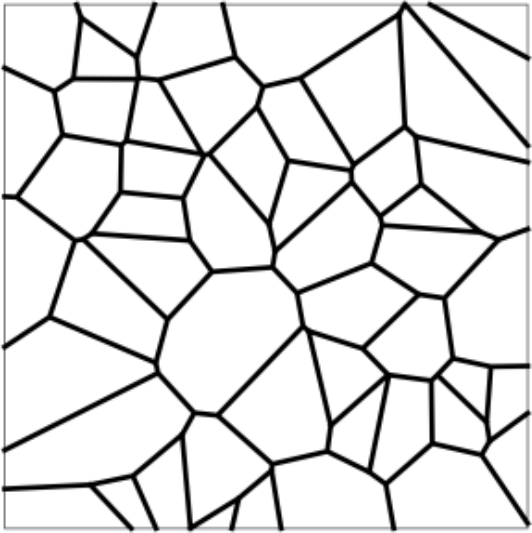
\includegraphics[height=5cm]{fig/voronoi-problem-rand}}
  \hfill
  \subcaptionbox{\label{fig:eval.studies.voronoi.prob.1attr}%
    Randomly distributed points with one attractor point in the bottom-left.}
    {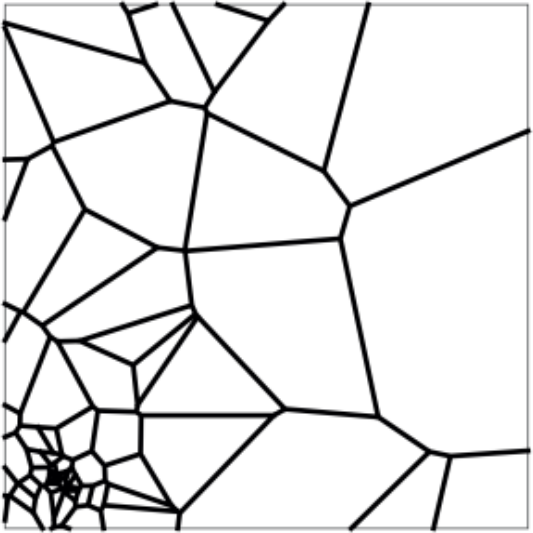
\includegraphics[height=5cm]{fig/voronoi-problem-1attr}}
  \hfill
  \subcaptionbox{\label{fig:eval.studies.voronoi.prob.edge}%
    Randomly distributed points with an attractor line at the bottom.}
    {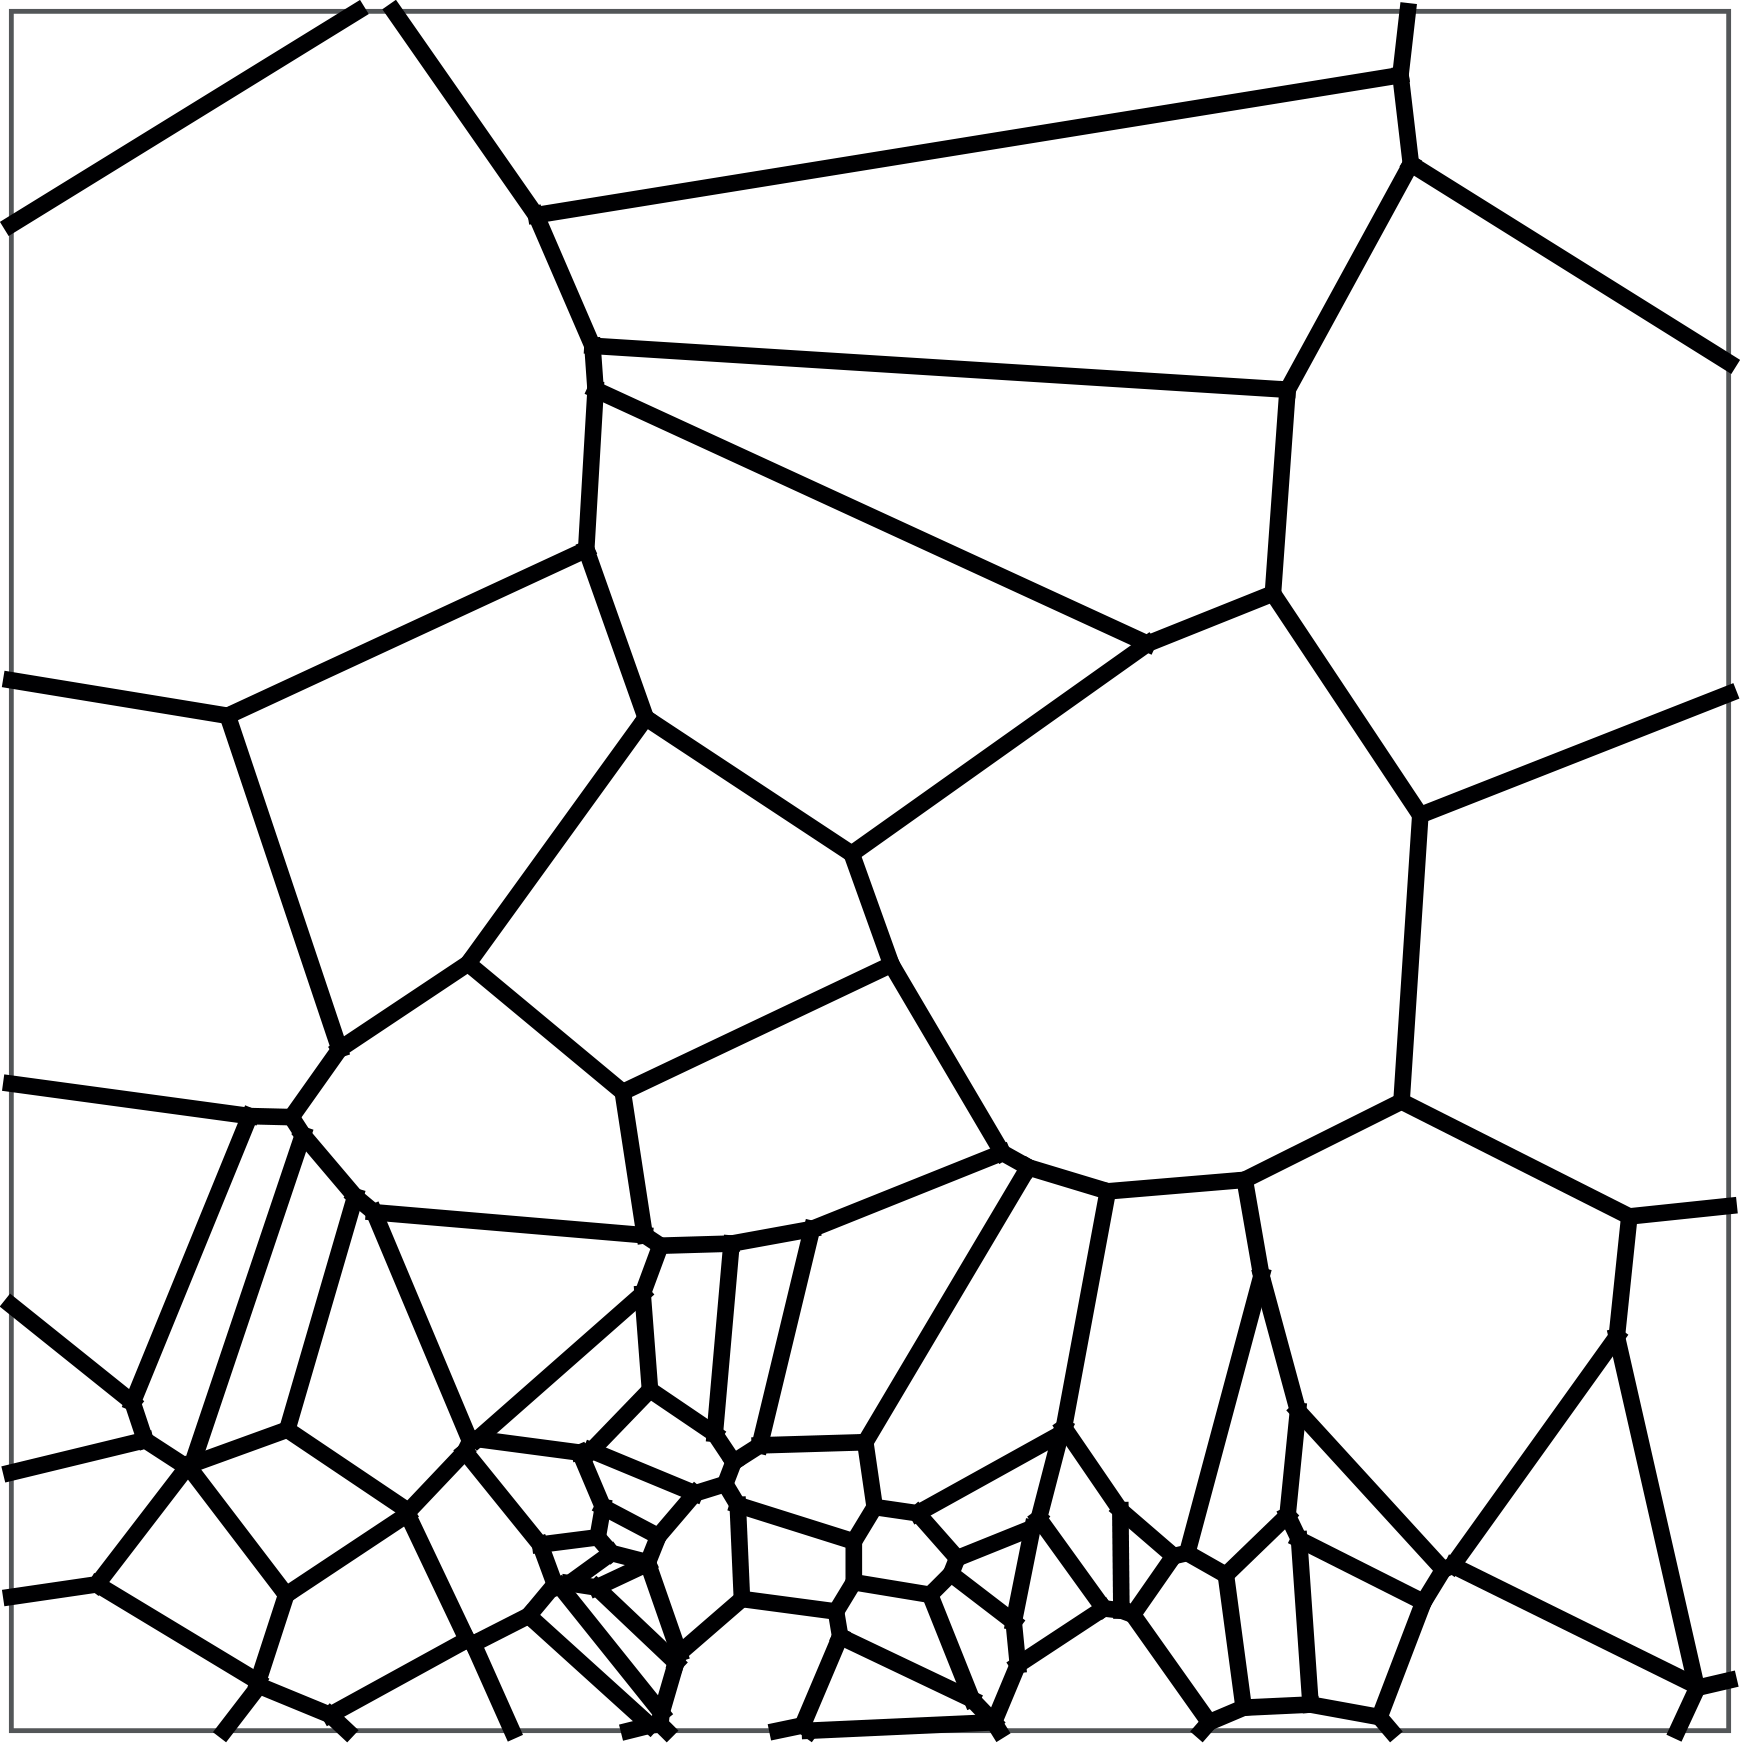
\includegraphics[height=5cm]{fig/voronoi-problem-edge}}
  \caption[Voronoi diagram problem]{
    Voronoi diagram problem: depicted are three Voronoi diagrams variations
    which are mostly generated at random.
    \subref{fig:eval.studies.voronoi.prob.rand} is entirely random,
    \subref{fig:eval.studies.voronoi.prob.1attr} expands on the latter with an
    attractor point, and \subref{fig:eval.studies.voronoi.prob.edge} goes even
    further by using an entire attractor line.}%
  \label{fig:eval.studies.voronoi.prob}
\end{figure}

Both the analytic and constructive methods focus on computation of a vertex
relies on the computation of the \textit{circumcenter} of a triangle, for
instance, triangle $\triangle P_1 P_2 P_3$
(\cref{fig:eval.studies.voronoi.sol}).

\begin{figure}[htb]
  \centering
  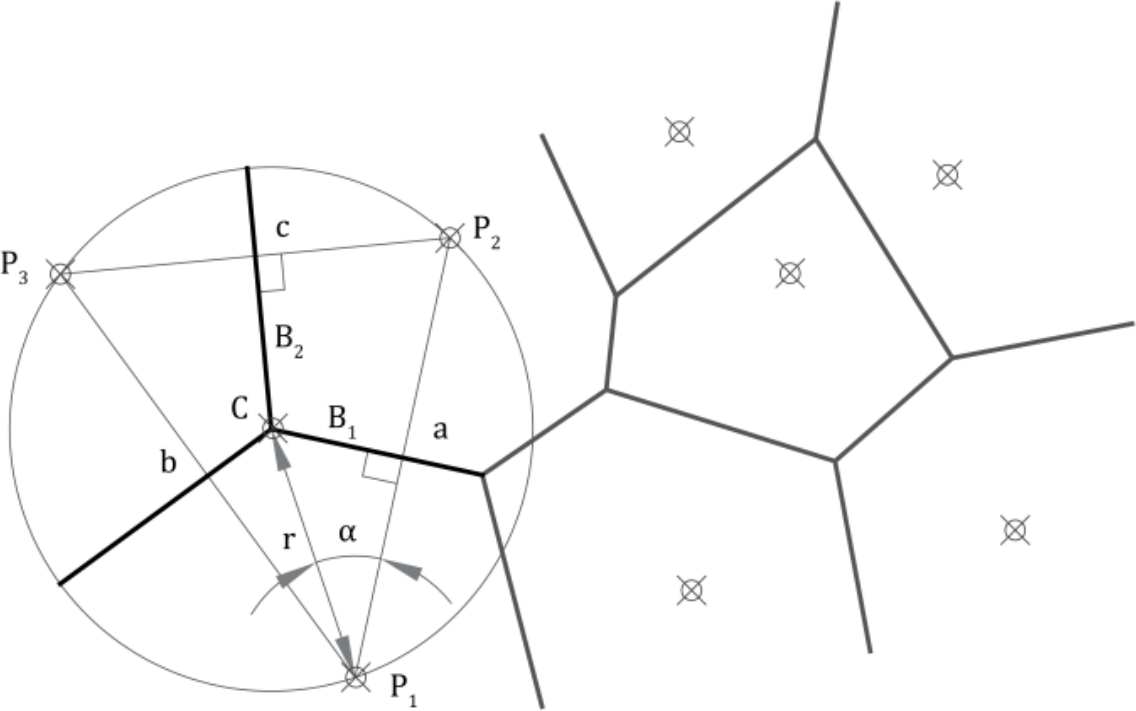
\includegraphics[height=6cm]{fig/voronoi-solution}
  \caption[Voronoi problem partial solution]{
    Analytic and constructive approaches to computing a Voronoi vertex via
    computing the circumcenter of every triangle in the Delaunay triangulation
    whose vertices are the Voronoi diagram's sites.}%
  \label{fig:eval.studies.voronoi.sol}
\end{figure}

There are several possible \textit{analytic solution} to compute a triangle's
circumcenter.  One of them is based on the \textit{circumradius} formula (step
\ref{enum:eval.studies.voronoi.sol.a.circum}), where $a$, $b$, and $c$ are the
lengths of the triangle's sides (step
\ref{enum:eval.studies.voronoi.sol.a.tri}) and $A$ is the triangle's area (step
\ref{enum:eval.studies.voronoi.sol.a.area}).  The circumcenter $C$ can then be
easily computed by a translation (step
\ref{enum:eval.studies.voronoi.sol.a.move}) from $P_1$ following the angle
$\alpha$ (step \ref{enum:eval.studies.voronoi.sol.a.alpha}).

\begin{enumerate}
  \item $a, b, c = \lVert P_2 - P_1 \rVert, \lVert P_3 - P_1 \rVert, \lVert P_3
  - P_2 \rVert$%
  \label{enum:eval.studies.voronoi.sol.a.tri}
  \item $s = \frac{a + b + c}{2}$
  \item $A = \sqrt{s(s - a)(s - b)(s - c)}$%
  \label{enum:eval.studies.voronoi.sol.a.area}
  \item $r = \frac{abc}{4A}$%
  \label{enum:eval.studies.voronoi.sol.a.circum}
  \item $\alpha = \arccos\frac{a}{2r}$%
  \label{enum:eval.studies.voronoi.sol.a.alpha}
  \item $C = P_1 + \left(r, \angle\alpha\right)$%
  \label{enum:eval.studies.voronoi.sol.a.move}
\end{enumerate}

The \textit{constructive solution} computes the circumcenter, given by the
intersection of the edges' perpendicular bisectors.  In fact, this has been
exemplified in \cref{chap:intro}.  Two \ac{GC} primitives were employed in this
solution, namely \textit{bisector} and \textit{intersection}.

\begin{enumerate}
  \item $B_1 = \mathrm{bisector}\left(\overline{P_1 P_2}\right)$
  \item $B_2 = \mathrm{bisector}\left(\overline{P_2 P_3}\right)$
  \item $C = \mathrm{intersection}\left(B_1, B_2\right)$
\end{enumerate}

We can increase the abstraction level of the solution by using the
\textit{circumcenter} functionality implemented in our solution, which, in
reality, is implemented in \ac{CGAL}:

\begin{enumerate}
  \item $C = \mathrm{circumcenter}\left(P_1, P_2, P_3\right)$
\end{enumerate}

The circumcenter problem is only a small part of the generation of a Voronoi
diagram, since we first need to build a Delaunay triangulation.  We can then 
apply the $\mathrm{circumcenter}$ functionality to find the Voronoi vertices and
draw the diagram's edges.  This set of steps can be abstracted away in a
functionality called \textit{voronoi} that, given a set of points $P_S$,
produces a 2D Euclidean Voronoi diagram:

\begin{enumerate}
  \item $V = \mathrm{voronoi}\left(P_S\right)$
\end{enumerate}

Implementing this functionality from scratch is a demanding and error-prone
task.  Fortunately, \ac{CGAL} already has an algorithm that produces robust 2D
Euclidean Voronoi diagrams that can handle degenerate cases, such as dealing
with three or more collinear points.  This algorithm, much like the
\textit{circumcenter} functionality, was entirely repurposed, and made available
in \texttt{CGAL.jl}, and, thus, it is also available in our solution.

% !TeX root = ../../main.tex
\section{Voronoi Diagrams Extended}%
\label{sec:eval.voronoi}

In the previous section, we left the problem of Voronoi Diagrams partially
unresolved, only tackling a small sub-problem required for computing the
diagram's vertices.  This section expands on it by showing how we can repurpose
\ac{CGAL}'s version of the Voronoi Diagram algorithm~\cite{CGAL:5.3:VDA2} as a
beneficial side effect of integrating with the library.  Additionally, we
compare said version with a native Julia implementation of the algorithm
described in~\cite{Springel:2010:GCHSMM} available in the
\texttt{VoronoiDelaunay.jl}\footnote{\url{https://github.com/JuliaGeometry/VoronoiDelaunay.jl}}
package.  Measurements involved obtaining an estimate of the effort required to
create either implementation, measuring Delaunay Triangulation construction
performance, and subsequent output triangulation and diagram comparison.

Both implementations adopt a similar incremental approach and are both robust.
The version from \texttt{VoronoiDelaunay.jl}, however, uses floating point
filtering~\cite{Springel:2010:GCHSMM}, requiring all point coordinates to be in
the interval $\left(1, 2\right) \times \left(1, 2\right) \subset \mathbb{R}^2$;
a restriction \ac{CGAL}'s implementation does not have since it uses a dynamic
floating point precision approach\footnote{Briefed at
\url{https://www.cs.cmu.edu/~quake/robust.html}}~\cite{Shewchuk:1997:APFPAFRGP}.
The \textit{limitation} in the former arguably constitutes a minor inconvenience
since the diagram may be produced in that limited range and then scaled
afterwards to meet the use case's needs.  But it is worth noting the issue is
not present in \ac{CGAL}'s implementation.  This is relevant if the input
coordinates cannot be altered to meet those needs.

To illustrate how we obtained the 2D Delaunay Triangulation and Voronoi Diagram
algorithms from \ac{CGAL}, \cref{lst:appendix.voronoi.jlcxx} shows a minimal
working example of the wrapper library code supported by JlCxx required to make
the necessary constructs and functionality available in Julia.  It follows a
familiar approach, the same used to obtain the core constructs supporting our
\primitives{} solution.  \Cref{lst:eval.voronoi.jl} shows a bare-bones Julia
module encapsulating and exposing the mapped functionality to the Julia
language.
\begin{listing}[htb]
  \inputminted{julia}{jl/Voronoi.jl}
  \caption[Bare-bones Julia module wrapping CGAL's Delaunay algorithms]{
    Bare-bones Julia module wrapping \ac{CGAL}'s 2D Delaunay Triangulation and
    Voronoi Diagrams, supported by the JlCxx wrapper in
    \cref{lst:appendix.voronoi.jlcxx}.}%
  \label{lst:eval.voronoi.jl}
\end{listing}
\texttt{CGAL.jl} contains a version of these mappings that are, however,
parameterized, and adds methods for querying, insertion, and further
manipulation.  For the purposes of testing, we used the slimmer \texttt{Voronoi}
module (\cref{lst:eval.voronoi.jl}).

The process for obtaining these bindings is a relatively simple one that
requires bare minimal C++ knowledge and following reference documentation as if
it were a recipe book, looking up the necessary ingredients and adding them to
the mix.  Accounting for trial and error, in case a minute detail was
overlooked, to make this functionality available would take no more than a full
day.  Having that, the algorithms are ready and available for use.

The algorithm present in \texttt{VoronoiDelaunay.jl} is the result of an immense
body of research, detailed in the \textsc{Arepo}
paper~\cite{Springel:2010:GCHSMM}.  Julia is an expressive language that greatly
benefits prototyping.  Changes are easy to apply and test without the overhead
of compilation, a downside of prototyping in C++, especially when compiling
(against) a sizeable codebase.  We can only infer that the development of the
algorithm did not take long to draft.  However, we can certainly say that it
took more than a full day to obtain a robust implementation, far exceeding the
effort taken by just repurposing an existing robust implementation in \ac{CGAL}.
It required interpretation and understanding of the approach described in the
article since there is no explicit algorithm listed.  This then requires the
creation of a conceptual mapping of the algorithm's entities and procedures,
later translating them into corresponding, preferably efficient, data structures
and functions in the Julia language.  These are among other trials and
tribulations that we did not have to meet in the slightest.  Our estimate is
that developing the algorithm in \texttt{VoronoiDelaunay.jl} took far longer
than obtaining one via our approach.

Regarding both algorithms' performance, \cref{tab:eval.voronoi.bench} shows a
series of results obtained by batch inserting various powers-of-ten sets of
points into Delaunay Triangulation objects, effectively building the meshes.
The results are plotted in \cref{fig:eval.voronoi.bench} for a better
understanding of the tabulated results.  The source code used to perform these
tests is listed in \cref{lst:appendix.voronoi.benchjl}.  More detailed data can
be seen in \cref{lst:appendix.voronoi.data}.

\begin{table}[htb]
  \caption[Delaunay Triangulation benchmarks]{
    Execution times for the construction of Delaunay Triangulations, comparing
    implementations of the algorithm: one from \ac{CGAL} and one from
    \texttt{VoronoiDelaunay.jl}.}%
  \label{tab:eval.voronoi.bench}
  \centering
  \begin{tabular}{r*{2}{l}}
    \toprule
    \multirow{2}{*}{\textbf{\# Points}}
    & \multicolumn{2}{c}{\textbf{Execution time (mean ± σ)}} \\
    & \multicolumn{1}{c}{\texttt{Voronoi.jl}}
    & \multicolumn{1}{c}{\texttt{VoronoiDelaunay.jl}} \\
    \midrule
    10\textsuperscript{2} & \verb| 42.145 μs ±  5.638 μs|
                          & \verb| 53.799 μs ±  39.811 μs| \\
    10\textsuperscript{3} & \verb|509.757 μs ±  1.258 ms|
                          & \verb|510.851 μs ± 113.523 μs| \\
    10\textsuperscript{4} & \verb|  5.879 ms ±  3.874 ms|
                          & \verb|  5.606 ms ± 382.603 μs| \\
    10\textsuperscript{5} & \verb| 62.344 ms ± 11.980 ms|
                          & \verb| 65.103 ms ±   2.287 ms| \\
    10\textsuperscript{6} & \verb|668.331 ms ± 44.458 ms|
                          & \verb|841.925 ms ±  51.394 ms| \\
    \bottomrule
  \end{tabular}
\end{table}

\begin{figure}[htb]
  \centering
  \begin{tikzpicture}
  \begin{loglogaxis}[ybar=0pt,
    title={\texttt{Voronoi.jl} vs.\ \texttt{VoronoiDelaunay.jl}},
    xlabel={Number of Points (log)},
    ylabel={Average Time (ns, log)},
    width={\linewidth},
    height=6cm,
    bar width=3.16227766,% 10^(1/n) where n = 2 (bars)
    enlarge y limits={.2,upper},
    enlarge x limits={abs=3.16227766},
    legend columns=-1,
    table/col sep=comma,
    error bars/y explicit,
    error bars/y dir=both
  ]
    \addplot+ table [y error index=2] {data/voronoi-vdjl.csv};
    \addplot+ table [y error index=2] {data/voronoi-cgal.csv};
    \legend{VoronoiDelaunay.jl,Voronoi.jl}
  \end{loglogaxis}
  \end{tikzpicture}
  \caption[Delaunay Triangulation benchmarks]{
    Delaunay Triangulation benchmark comparison results collected form
    \cref{tab:eval.voronoi.bench} in a Y-bar plot.  Both axes follow a
    logarithmic scale.}%
  \label{fig:eval.voronoi.bench}
\end{figure}

The sets of points were randomly generated using an instance of the Mersenne
Twister pseudo-random number generator, MT19937, with the seed
\texttt{0xdeadbeef}.  Tests for 10\textsuperscript{n} points used the same
10\textsuperscript{n} random points for every sample evaluated.  Results are
pretty identical, both variants trading blows.  However, more often than not, we
see \ac{CGAL}'s variant of the algorithm beating \texttt{VoronoiDelaunay.jl}'s
by a relatively small margin, except the last result's difference is more than
marginal.  We see some more variation from \ac{CGAL}'s algorithm, but looking at
more detailed data (\cref{lst:appendix.voronoi.data}), such cases seem to be
punctual at best, proving negligible in practice.

One other interesting detail we can see represented in additional data is that
of estimated memory usage.  The algorithm in \texttt{VoronoiDelaunay.jl} appears
to use far more memory than \ac{CGAL}'s does, differing by two entire orders of
magnitude.  We did not investigate any further, though additional profiling
could help bring light to some of these results.

Finally, we take a look at the output Delaunay Triangulations and their
respective dual Voronoi Diagrams, produced by both implementations.
\Cref{fig:eval.voronoi.output} illustrates two plots of overlapping meshes: on
the left, the Delaunay Triangulations, and on the right, the respective dual
Voronoi Diagrams.

\begin{figure}[!htb]
  \resizebox{\linewidth}{!}{\begin{tikzpicture}[/tikz/background rectangle/.style={fill={rgb,1:red,1.0;green,1.0;blue,1.0}, draw opacity={1.0}}, show background rectangle]
\begin{axis}[point meta max={nan}, point meta min={nan}, title={Delaunay Triangulation}, title style={at={{(0.5,1)}}, anchor={south}, font={{\fontsize{10 pt}{13.0 pt}\selectfont}}, color={rgb,1:red,0.0;green,0.0;blue,0.0}, draw opacity={1.0}, rotate={0.0}}, legend style={color={rgb,1:red,0.0;green,0.0;blue,0.0}, draw opacity={1.0}, line width={1}, solid, fill={rgb,1:red,1.0;green,1.0;blue,1.0}, fill opacity={1.0}, text opacity={1.0}, font={{\fontsize{8 pt}{10.4 pt}\selectfont}}, text={rgb,1:red,0.0;green,0.0;blue,0.0}, cells={anchor={west}}, at={(0.98, 0.98)}, anchor={north east}}, axis background/.style={fill={rgb,1:red,1.0;green,1.0;blue,1.0}, opacity={1.0}}, anchor={north west}, xshift={1.0mm}, yshift={-1.0mm}, width={86.9mm}, height={86.9mm}, scaled x ticks={false}, xlabel={$x$}, x tick style={color={rgb,1:red,0.0;green,0.0;blue,0.0}, opacity={1.0}}, x tick label style={color={rgb,1:red,0.0;green,0.0;blue,0.0}, opacity={1.0}, rotate={0}}, xlabel style={at={(ticklabel cs:0.5)}, anchor=near ticklabel, font={{\fontsize{11 pt}{14.3 pt}\selectfont}}, color={rgb,1:red,0.0;green,0.0;blue,0.0}, draw opacity={1.0}, rotate={0.0}}, xmajorgrids={true}, xmin={0.9}, xmax={2.1}, xtick={{1.0,1.25,1.5,1.75,2.0}}, xticklabels={{$1.00$,$1.25$,$1.50$,$1.75$,$2.00$}}, xtick align={inside}, xticklabel style={font={{\fontsize{8 pt}{10.4 pt}\selectfont}}, color={rgb,1:red,0.0;green,0.0;blue,0.0}, draw opacity={1.0}, rotate={0.0}}, x grid style={color={rgb,1:red,0.0;green,0.0;blue,0.0}, draw opacity={0.1}, line width={0.5}, solid}, axis x line*={left}, x axis line style={color={rgb,1:red,0.0;green,0.0;blue,0.0}, draw opacity={1.0}, line width={1}, solid}, scaled y ticks={false}, ylabel={$y$}, y tick style={color={rgb,1:red,0.0;green,0.0;blue,0.0}, opacity={1.0}}, y tick label style={color={rgb,1:red,0.0;green,0.0;blue,0.0}, opacity={1.0}, rotate={0}}, ylabel style={at={(ticklabel cs:0.5)}, anchor=near ticklabel, font={{\fontsize{11 pt}{14.3 pt}\selectfont}}, color={rgb,1:red,0.0;green,0.0;blue,0.0}, draw opacity={1.0}, rotate={0.0}}, ymajorgrids={true}, ymin={0.9}, ymax={2.1}, ytick={{1.0,1.25,1.5,1.75,2.0}}, yticklabels={{$1.00$,$1.25$,$1.50$,$1.75$,$2.00$}}, ytick align={inside}, yticklabel style={font={{\fontsize{8 pt}{10.4 pt}\selectfont}}, color={rgb,1:red,0.0;green,0.0;blue,0.0}, draw opacity={1.0}, rotate={0.0}}, y grid style={color={rgb,1:red,0.0;green,0.0;blue,0.0}, draw opacity={0.1}, line width={0.5}, solid}, axis y line*={left}, y axis line style={color={rgb,1:red,0.0;green,0.0;blue,0.0}, draw opacity={1.0}, line width={1}, solid}, colorbar={false}, legend columns={-1}]
    \addplot[color={rgb,1:red,1.0;green,0.0;blue,0.0}, name path={feac98d9-325b-42e4-8488-6ffcf40c5241}, draw opacity={1.0}, line width={1}, solid]
        table[row sep={\\}]
        {
            \\
            1.1748122130520642  1.9119394752196963  \\
            1.3983968361280859  1.8132919843774284  \\
        }
        ;
    \addlegendentry {Voronoi.jl}
    \addplot[color={rgb,1:red,1.0;green,0.0;blue,0.0}, name path={feac98d9-325b-42e4-8488-6ffcf40c5241}, draw opacity={1.0}, line width={1}, solid, forget plot]
        table[row sep={\\}]
        {
            \\
            1.3983968361280859  1.8132919843774284  \\
            1.3702157551888376  1.9199406439438458  \\
        }
        ;
    \addplot[color={rgb,1:red,1.0;green,0.0;blue,0.0}, name path={feac98d9-325b-42e4-8488-6ffcf40c5241}, draw opacity={1.0}, line width={1}, solid, forget plot]
        table[row sep={\\}]
        {
            \\
            1.3702157551888376  1.9199406439438458  \\
            1.1748122130520642  1.9119394752196963  \\
        }
        ;
    \addplot[color={rgb,1:red,1.0;green,0.0;blue,0.0}, name path={feac98d9-325b-42e4-8488-6ffcf40c5241}, draw opacity={1.0}, line width={1}, solid, forget plot]
        table[row sep={\\}]
        {
            \\
            1.3983968361280859  1.8132919843774284  \\
            1.411079611396417  1.603287132689729  \\
        }
        ;
    \addplot[color={rgb,1:red,1.0;green,0.0;blue,0.0}, name path={feac98d9-325b-42e4-8488-6ffcf40c5241}, draw opacity={1.0}, line width={1}, solid, forget plot]
        table[row sep={\\}]
        {
            \\
            1.411079611396417  1.603287132689729  \\
            1.4094003408681601  1.8230532801244403  \\
        }
        ;
    \addplot[color={rgb,1:red,1.0;green,0.0;blue,0.0}, name path={feac98d9-325b-42e4-8488-6ffcf40c5241}, draw opacity={1.0}, line width={1}, solid, forget plot]
        table[row sep={\\}]
        {
            \\
            1.4094003408681601  1.8230532801244403  \\
            1.3983968361280859  1.8132919843774284  \\
        }
        ;
    \addplot[color={rgb,1:red,1.0;green,0.0;blue,0.0}, name path={feac98d9-325b-42e4-8488-6ffcf40c5241}, draw opacity={1.0}, line width={1}, solid, forget plot]
        table[row sep={\\}]
        {
            \\
            1.8946103360503908  1.4291503357235342  \\
            1.8488018650095905  1.693958807038143  \\
        }
        ;
    \addplot[color={rgb,1:red,1.0;green,0.0;blue,0.0}, name path={feac98d9-325b-42e4-8488-6ffcf40c5241}, draw opacity={1.0}, line width={1}, solid, forget plot]
        table[row sep={\\}]
        {
            \\
            1.8488018650095905  1.693958807038143  \\
            1.8273643609136339  1.502810534555465  \\
        }
        ;
    \addplot[color={rgb,1:red,1.0;green,0.0;blue,0.0}, name path={feac98d9-325b-42e4-8488-6ffcf40c5241}, draw opacity={1.0}, line width={1}, solid, forget plot]
        table[row sep={\\}]
        {
            \\
            1.8273643609136339  1.502810534555465  \\
            1.8946103360503908  1.4291503357235342  \\
        }
        ;
    \addplot[color={rgb,1:red,1.0;green,0.0;blue,0.0}, name path={feac98d9-325b-42e4-8488-6ffcf40c5241}, draw opacity={1.0}, line width={1}, solid, forget plot]
        table[row sep={\\}]
        {
            \\
            1.670456608990207  1.4213281597476453  \\
            1.8273643609136339  1.502810534555465  \\
        }
        ;
    \addplot[color={rgb,1:red,1.0;green,0.0;blue,0.0}, name path={feac98d9-325b-42e4-8488-6ffcf40c5241}, draw opacity={1.0}, line width={1}, solid, forget plot]
        table[row sep={\\}]
        {
            \\
            1.8273643609136339  1.502810534555465  \\
            1.7508308666292574  1.5433638719841838  \\
        }
        ;
    \addplot[color={rgb,1:red,1.0;green,0.0;blue,0.0}, name path={feac98d9-325b-42e4-8488-6ffcf40c5241}, draw opacity={1.0}, line width={1}, solid, forget plot]
        table[row sep={\\}]
        {
            \\
            1.7508308666292574  1.5433638719841838  \\
            1.670456608990207  1.4213281597476453  \\
        }
        ;
    \addplot[color={rgb,1:red,1.0;green,0.0;blue,0.0}, name path={feac98d9-325b-42e4-8488-6ffcf40c5241}, draw opacity={1.0}, line width={1}, solid, forget plot]
        table[row sep={\\}]
        {
            \\
            1.4094003408681601  1.8230532801244403  \\
            1.8488018650095905  1.693958807038143  \\
        }
        ;
    \addplot[color={rgb,1:red,1.0;green,0.0;blue,0.0}, name path={feac98d9-325b-42e4-8488-6ffcf40c5241}, draw opacity={1.0}, line width={1}, solid, forget plot]
        table[row sep={\\}]
        {
            \\
            1.8488018650095905  1.693958807038143  \\
            1.3702157551888376  1.9199406439438458  \\
        }
        ;
    \addplot[color={rgb,1:red,1.0;green,0.0;blue,0.0}, name path={feac98d9-325b-42e4-8488-6ffcf40c5241}, draw opacity={1.0}, line width={1}, solid, forget plot]
        table[row sep={\\}]
        {
            \\
            1.3702157551888376  1.9199406439438458  \\
            1.4094003408681601  1.8230532801244403  \\
        }
        ;
    \addplot[color={rgb,1:red,1.0;green,0.0;blue,0.0}, name path={feac98d9-325b-42e4-8488-6ffcf40c5241}, draw opacity={1.0}, line width={1}, solid, forget plot]
        table[row sep={\\}]
        {
            \\
            1.7508308666292574  1.5433638719841838  \\
            1.8488018650095905  1.693958807038143  \\
        }
        ;
    \addplot[color={rgb,1:red,1.0;green,0.0;blue,0.0}, name path={feac98d9-325b-42e4-8488-6ffcf40c5241}, draw opacity={1.0}, line width={1}, solid, forget plot]
        table[row sep={\\}]
        {
            \\
            1.4094003408681601  1.8230532801244403  \\
            1.7508308666292574  1.5433638719841838  \\
        }
        ;
    \addplot[color={rgb,1:red,1.0;green,0.0;blue,0.0}, name path={feac98d9-325b-42e4-8488-6ffcf40c5241}, draw opacity={1.0}, line width={1}, solid, forget plot]
        table[row sep={\\}]
        {
            \\
            1.6398598169907925  1.1640638990793377  \\
            1.8701207209378476  1.1696756919845939  \\
        }
        ;
    \addplot[color={rgb,1:red,1.0;green,0.0;blue,0.0}, name path={feac98d9-325b-42e4-8488-6ffcf40c5241}, draw opacity={1.0}, line width={1}, solid, forget plot]
        table[row sep={\\}]
        {
            \\
            1.8701207209378476  1.1696756919845939  \\
            1.670456608990207  1.4213281597476453  \\
        }
        ;
    \addplot[color={rgb,1:red,1.0;green,0.0;blue,0.0}, name path={feac98d9-325b-42e4-8488-6ffcf40c5241}, draw opacity={1.0}, line width={1}, solid, forget plot]
        table[row sep={\\}]
        {
            \\
            1.670456608990207  1.4213281597476453  \\
            1.6398598169907925  1.1640638990793377  \\
        }
        ;
    \addplot[color={rgb,1:red,1.0;green,0.0;blue,0.0}, name path={feac98d9-325b-42e4-8488-6ffcf40c5241}, draw opacity={1.0}, line width={1}, solid, forget plot]
        table[row sep={\\}]
        {
            \\
            1.1105229298118504  1.3180863440502435  \\
            1.5939507135190067  1.132305847713724  \\
        }
        ;
    \addplot[color={rgb,1:red,1.0;green,0.0;blue,0.0}, name path={feac98d9-325b-42e4-8488-6ffcf40c5241}, draw opacity={1.0}, line width={1}, solid, forget plot]
        table[row sep={\\}]
        {
            \\
            1.5939507135190067  1.132305847713724  \\
            1.3071074625477195  1.3007149568293244  \\
        }
        ;
    \addplot[color={rgb,1:red,1.0;green,0.0;blue,0.0}, name path={feac98d9-325b-42e4-8488-6ffcf40c5241}, draw opacity={1.0}, line width={1}, solid, forget plot]
        table[row sep={\\}]
        {
            \\
            1.3071074625477195  1.3007149568293244  \\
            1.1105229298118504  1.3180863440502435  \\
        }
        ;
    \addplot[color={rgb,1:red,1.0;green,0.0;blue,0.0}, name path={feac98d9-325b-42e4-8488-6ffcf40c5241}, draw opacity={1.0}, line width={1}, solid, forget plot]
        table[row sep={\\}]
        {
            \\
            1.3230645160656422  1.6671039194334296  \\
            1.1387269033584746  1.3902763912919909  \\
        }
        ;
    \addplot[color={rgb,1:red,1.0;green,0.0;blue,0.0}, name path={feac98d9-325b-42e4-8488-6ffcf40c5241}, draw opacity={1.0}, line width={1}, solid, forget plot]
        table[row sep={\\}]
        {
            \\
            1.1387269033584746  1.3902763912919909  \\
            1.4044450228102505  1.4121578056365252  \\
        }
        ;
    \addplot[color={rgb,1:red,1.0;green,0.0;blue,0.0}, name path={feac98d9-325b-42e4-8488-6ffcf40c5241}, draw opacity={1.0}, line width={1}, solid, forget plot]
        table[row sep={\\}]
        {
            \\
            1.4044450228102505  1.4121578056365252  \\
            1.3230645160656422  1.6671039194334296  \\
        }
        ;
    \addplot[color={rgb,1:red,1.0;green,0.0;blue,0.0}, name path={feac98d9-325b-42e4-8488-6ffcf40c5241}, draw opacity={1.0}, line width={1}, solid, forget plot]
        table[row sep={\\}]
        {
            \\
            1.5201537685934454  1.5121217011474073  \\
            1.4094003408681601  1.8230532801244403  \\
        }
        ;
    \addplot[color={rgb,1:red,1.0;green,0.0;blue,0.0}, name path={feac98d9-325b-42e4-8488-6ffcf40c5241}, draw opacity={1.0}, line width={1}, solid, forget plot]
        table[row sep={\\}]
        {
            \\
            1.411079611396417  1.603287132689729  \\
            1.5201537685934454  1.5121217011474073  \\
        }
        ;
    \addplot[color={rgb,1:red,1.0;green,0.0;blue,0.0}, name path={feac98d9-325b-42e4-8488-6ffcf40c5241}, draw opacity={1.0}, line width={1}, solid, forget plot]
        table[row sep={\\}]
        {
            \\
            1.5939507135190067  1.132305847713724  \\
            1.4044450228102505  1.4121578056365252  \\
        }
        ;
    \addplot[color={rgb,1:red,1.0;green,0.0;blue,0.0}, name path={feac98d9-325b-42e4-8488-6ffcf40c5241}, draw opacity={1.0}, line width={1}, solid, forget plot]
        table[row sep={\\}]
        {
            \\
            1.4044450228102505  1.4121578056365252  \\
            1.3071074625477195  1.3007149568293244  \\
        }
        ;
    \addplot[color={rgb,1:red,1.0;green,0.0;blue,0.0}, name path={feac98d9-325b-42e4-8488-6ffcf40c5241}, draw opacity={1.0}, line width={1}, solid, forget plot]
        table[row sep={\\}]
        {
            \\
            1.1387269033584746  1.3902763912919909  \\
            1.3071074625477195  1.3007149568293244  \\
        }
        ;
    \addplot[color={rgb,1:red,1.0;green,0.0;blue,0.0}, name path={feac98d9-325b-42e4-8488-6ffcf40c5241}, draw opacity={1.0}, line width={1}, solid, forget plot]
        table[row sep={\\}]
        {
            \\
            1.1387269033584746  1.3902763912919909  \\
            1.125095868483186  1.7752906912937756  \\
        }
        ;
    \addplot[color={rgb,1:red,1.0;green,0.0;blue,0.0}, name path={feac98d9-325b-42e4-8488-6ffcf40c5241}, draw opacity={1.0}, line width={1}, solid, forget plot]
        table[row sep={\\}]
        {
            \\
            1.125095868483186  1.7752906912937756  \\
            1.1105229298118504  1.3180863440502435  \\
        }
        ;
    \addplot[color={rgb,1:red,1.0;green,0.0;blue,0.0}, name path={feac98d9-325b-42e4-8488-6ffcf40c5241}, draw opacity={1.0}, line width={1}, solid, forget plot]
        table[row sep={\\}]
        {
            \\
            1.1105229298118504  1.3180863440502435  \\
            1.1387269033584746  1.3902763912919909  \\
        }
        ;
    \addplot[color={rgb,1:red,1.0;green,0.0;blue,0.0}, name path={feac98d9-325b-42e4-8488-6ffcf40c5241}, draw opacity={1.0}, line width={1}, solid, forget plot]
        table[row sep={\\}]
        {
            \\
            1.3230645160656422  1.6671039194334296  \\
            1.125095868483186  1.7752906912937756  \\
        }
        ;
    \addplot[color={rgb,1:red,1.0;green,0.0;blue,0.0}, name path={feac98d9-325b-42e4-8488-6ffcf40c5241}, draw opacity={1.0}, line width={1}, solid, forget plot]
        table[row sep={\\}]
        {
            \\
            1.3983968361280859  1.8132919843774284  \\
            1.125095868483186  1.7752906912937756  \\
        }
        ;
    \addplot[color={rgb,1:red,1.0;green,0.0;blue,0.0}, name path={feac98d9-325b-42e4-8488-6ffcf40c5241}, draw opacity={1.0}, line width={1}, solid, forget plot]
        table[row sep={\\}]
        {
            \\
            1.3230645160656422  1.6671039194334296  \\
            1.3983968361280859  1.8132919843774284  \\
        }
        ;
    \addplot[color={rgb,1:red,1.0;green,0.0;blue,0.0}, name path={feac98d9-325b-42e4-8488-6ffcf40c5241}, draw opacity={1.0}, line width={1}, solid, forget plot]
        table[row sep={\\}]
        {
            \\
            1.4235251017380506  1.5806863505858928  \\
            1.5201537685934454  1.5121217011474073  \\
        }
        ;
    \addplot[color={rgb,1:red,1.0;green,0.0;blue,0.0}, name path={feac98d9-325b-42e4-8488-6ffcf40c5241}, draw opacity={1.0}, line width={1}, solid, forget plot]
        table[row sep={\\}]
        {
            \\
            1.411079611396417  1.603287132689729  \\
            1.4235251017380506  1.5806863505858928  \\
        }
        ;
    \addplot[color={rgb,1:red,1.0;green,0.0;blue,0.0}, name path={feac98d9-325b-42e4-8488-6ffcf40c5241}, draw opacity={1.0}, line width={1}, solid, forget plot]
        table[row sep={\\}]
        {
            \\
            1.125095868483186  1.7752906912937756  \\
            1.1748122130520642  1.9119394752196963  \\
        }
        ;
    \addplot[color={rgb,1:red,1.0;green,0.0;blue,0.0}, name path={feac98d9-325b-42e4-8488-6ffcf40c5241}, draw opacity={1.0}, line width={1}, solid, forget plot]
        table[row sep={\\}]
        {
            \\
            1.4235251017380506  1.5806863505858928  \\
            1.3230645160656422  1.6671039194334296  \\
        }
        ;
    \addplot[color={rgb,1:red,1.0;green,0.0;blue,0.0}, name path={feac98d9-325b-42e4-8488-6ffcf40c5241}, draw opacity={1.0}, line width={1}, solid, forget plot]
        table[row sep={\\}]
        {
            \\
            1.4044450228102505  1.4121578056365252  \\
            1.4235251017380506  1.5806863505858928  \\
        }
        ;
    \addplot[color={rgb,1:red,1.0;green,0.0;blue,0.0}, name path={feac98d9-325b-42e4-8488-6ffcf40c5241}, draw opacity={1.0}, line width={1}, solid, forget plot]
        table[row sep={\\}]
        {
            \\
            1.5201537685934454  1.5121217011474073  \\
            1.7508308666292574  1.5433638719841838  \\
        }
        ;
    \addplot[color={rgb,1:red,1.0;green,0.0;blue,0.0}, name path={feac98d9-325b-42e4-8488-6ffcf40c5241}, draw opacity={1.0}, line width={1}, solid, forget plot]
        table[row sep={\\}]
        {
            \\
            1.4044450228102505  1.4121578056365252  \\
            1.5201537685934454  1.5121217011474073  \\
        }
        ;
    \addplot[color={rgb,1:red,1.0;green,0.0;blue,0.0}, name path={feac98d9-325b-42e4-8488-6ffcf40c5241}, draw opacity={1.0}, line width={1}, solid, forget plot]
        table[row sep={\\}]
        {
            \\
            1.670456608990207  1.4213281597476453  \\
            1.4044450228102505  1.4121578056365252  \\
        }
        ;
    \addplot[color={rgb,1:red,1.0;green,0.0;blue,0.0}, name path={feac98d9-325b-42e4-8488-6ffcf40c5241}, draw opacity={1.0}, line width={1}, solid, forget plot]
        table[row sep={\\}]
        {
            \\
            1.4044450228102505  1.4121578056365252  \\
            1.6398598169907925  1.1640638990793377  \\
        }
        ;
    \addplot[color={rgb,1:red,1.0;green,0.0;blue,0.0}, name path={feac98d9-325b-42e4-8488-6ffcf40c5241}, draw opacity={1.0}, line width={1}, solid, forget plot]
        table[row sep={\\}]
        {
            \\
            1.3230645160656422  1.6671039194334296  \\
            1.411079611396417  1.603287132689729  \\
        }
        ;
    \addplot[color={rgb,1:red,1.0;green,0.0;blue,0.0}, name path={feac98d9-325b-42e4-8488-6ffcf40c5241}, draw opacity={1.0}, line width={1}, solid, forget plot]
        table[row sep={\\}]
        {
            \\
            1.670456608990207  1.4213281597476453  \\
            1.8946103360503908  1.4291503357235342  \\
        }
        ;
    \addplot[color={rgb,1:red,1.0;green,0.0;blue,0.0}, name path={feac98d9-325b-42e4-8488-6ffcf40c5241}, draw opacity={1.0}, line width={1}, solid, forget plot]
        table[row sep={\\}]
        {
            \\
            1.8946103360503908  1.4291503357235342  \\
            1.8701207209378476  1.1696756919845939  \\
        }
        ;
    \addplot[color={rgb,1:red,1.0;green,0.0;blue,0.0}, name path={feac98d9-325b-42e4-8488-6ffcf40c5241}, draw opacity={1.0}, line width={1}, solid, forget plot]
        table[row sep={\\}]
        {
            \\
            1.5201537685934454  1.5121217011474073  \\
            1.670456608990207  1.4213281597476453  \\
        }
        ;
    \addplot[color={rgb,1:red,1.0;green,0.0;blue,0.0}, name path={feac98d9-325b-42e4-8488-6ffcf40c5241}, draw opacity={1.0}, line width={1}, solid, forget plot]
        table[row sep={\\}]
        {
            \\
            1.5939507135190067  1.132305847713724  \\
            1.8701207209378476  1.1696756919845939  \\
        }
        ;
    \addplot[color={rgb,1:red,1.0;green,0.0;blue,0.0}, name path={feac98d9-325b-42e4-8488-6ffcf40c5241}, draw opacity={1.0}, line width={1}, solid, forget plot]
        table[row sep={\\}]
        {
            \\
            1.6398598169907925  1.1640638990793377  \\
            1.5939507135190067  1.132305847713724  \\
        }
        ;
    \addplot[color={rgb,1:red,0.0;green,1.0;blue,0.498}, name path={36c44fbf-fb68-45d6-8a13-8daff49c720f}, draw opacity={0.8}, line width={1}, solid]
        table[row sep={\\}]
        {
            \\
            1.670456608990207  1.4213281597476453  \\
            1.7508308666292574  1.5433638719841838  \\
        }
        ;
    \addlegendentry {VoronoiDelaunay.jl}
    \addplot[color={rgb,1:red,0.0;green,1.0;blue,0.498}, name path={36c44fbf-fb68-45d6-8a13-8daff49c720f}, draw opacity={0.8}, line width={1}, solid, forget plot]
        table[row sep={\\}]
        {
            \\
            1.8273643609136339  1.502810534555465  \\
            1.7508308666292574  1.5433638719841838  \\
        }
        ;
    \addplot[color={rgb,1:red,0.0;green,1.0;blue,0.498}, name path={36c44fbf-fb68-45d6-8a13-8daff49c720f}, draw opacity={0.8}, line width={1}, solid, forget plot]
        table[row sep={\\}]
        {
            \\
            1.8273643609136339  1.502810534555465  \\
            1.670456608990207  1.4213281597476453  \\
        }
        ;
    \addplot[color={rgb,1:red,0.0;green,1.0;blue,0.498}, name path={36c44fbf-fb68-45d6-8a13-8daff49c720f}, draw opacity={0.8}, line width={1}, solid, forget plot]
        table[row sep={\\}]
        {
            \\
            1.3702157551888376  1.9199406439438458  \\
            1.4094003408681601  1.8230532801244403  \\
        }
        ;
    \addplot[color={rgb,1:red,0.0;green,1.0;blue,0.498}, name path={36c44fbf-fb68-45d6-8a13-8daff49c720f}, draw opacity={0.8}, line width={1}, solid, forget plot]
        table[row sep={\\}]
        {
            \\
            1.3983968361280859  1.8132919843774284  \\
            1.4094003408681601  1.8230532801244403  \\
        }
        ;
    \addplot[color={rgb,1:red,0.0;green,1.0;blue,0.498}, name path={36c44fbf-fb68-45d6-8a13-8daff49c720f}, draw opacity={0.8}, line width={1}, solid, forget plot]
        table[row sep={\\}]
        {
            \\
            1.3983968361280859  1.8132919843774284  \\
            1.3702157551888376  1.9199406439438458  \\
        }
        ;
    \addplot[color={rgb,1:red,0.0;green,1.0;blue,0.498}, name path={36c44fbf-fb68-45d6-8a13-8daff49c720f}, draw opacity={0.8}, line width={1}, solid, forget plot]
        table[row sep={\\}]
        {
            \\
            1.7508308666292574  1.5433638719841838  \\
            1.5201537685934454  1.5121217011474073  \\
        }
        ;
    \addplot[color={rgb,1:red,0.0;green,1.0;blue,0.498}, name path={36c44fbf-fb68-45d6-8a13-8daff49c720f}, draw opacity={0.8}, line width={1}, solid, forget plot]
        table[row sep={\\}]
        {
            \\
            1.4094003408681601  1.8230532801244403  \\
            1.5201537685934454  1.5121217011474073  \\
        }
        ;
    \addplot[color={rgb,1:red,0.0;green,1.0;blue,0.498}, name path={36c44fbf-fb68-45d6-8a13-8daff49c720f}, draw opacity={0.8}, line width={1}, solid, forget plot]
        table[row sep={\\}]
        {
            \\
            1.4094003408681601  1.8230532801244403  \\
            1.7508308666292574  1.5433638719841838  \\
        }
        ;
    \addplot[color={rgb,1:red,0.0;green,1.0;blue,0.498}, name path={36c44fbf-fb68-45d6-8a13-8daff49c720f}, draw opacity={0.8}, line width={1}, solid, forget plot]
        table[row sep={\\}]
        {
            \\
            1.670456608990207  1.4213281597476453  \\
            1.5201537685934454  1.5121217011474073  \\
        }
        ;
    \addplot[color={rgb,1:red,0.0;green,1.0;blue,0.498}, name path={36c44fbf-fb68-45d6-8a13-8daff49c720f}, draw opacity={0.8}, line width={1}, solid, forget plot]
        table[row sep={\\}]
        {
            \\
            1.411079611396417  1.603287132689729  \\
            1.4094003408681601  1.8230532801244403  \\
        }
        ;
    \addplot[color={rgb,1:red,0.0;green,1.0;blue,0.498}, name path={36c44fbf-fb68-45d6-8a13-8daff49c720f}, draw opacity={0.8}, line width={1}, solid, forget plot]
        table[row sep={\\}]
        {
            \\
            1.5201537685934454  1.5121217011474073  \\
            1.411079611396417  1.603287132689729  \\
        }
        ;
    \addplot[color={rgb,1:red,0.0;green,1.0;blue,0.498}, name path={36c44fbf-fb68-45d6-8a13-8daff49c720f}, draw opacity={0.8}, line width={1}, solid, forget plot]
        table[row sep={\\}]
        {
            \\
            1.4235251017380506  1.5806863505858928  \\
            1.3230645160656422  1.6671039194334296  \\
        }
        ;
    \addplot[color={rgb,1:red,0.0;green,1.0;blue,0.498}, name path={36c44fbf-fb68-45d6-8a13-8daff49c720f}, draw opacity={0.8}, line width={1}, solid, forget plot]
        table[row sep={\\}]
        {
            \\
            1.411079611396417  1.603287132689729  \\
            1.3230645160656422  1.6671039194334296  \\
        }
        ;
    \addplot[color={rgb,1:red,0.0;green,1.0;blue,0.498}, name path={36c44fbf-fb68-45d6-8a13-8daff49c720f}, draw opacity={0.8}, line width={1}, solid, forget plot]
        table[row sep={\\}]
        {
            \\
            1.411079611396417  1.603287132689729  \\
            1.4235251017380506  1.5806863505858928  \\
        }
        ;
    \addplot[color={rgb,1:red,0.0;green,1.0;blue,0.498}, name path={36c44fbf-fb68-45d6-8a13-8daff49c720f}, draw opacity={0.8}, line width={1}, solid, forget plot]
        table[row sep={\\}]
        {
            \\
            1.4044450228102505  1.4121578056365252  \\
            1.670456608990207  1.4213281597476453  \\
        }
        ;
    \addplot[color={rgb,1:red,0.0;green,1.0;blue,0.498}, name path={36c44fbf-fb68-45d6-8a13-8daff49c720f}, draw opacity={0.8}, line width={1}, solid, forget plot]
        table[row sep={\\}]
        {
            \\
            1.6398598169907925  1.1640638990793377  \\
            1.670456608990207  1.4213281597476453  \\
        }
        ;
    \addplot[color={rgb,1:red,0.0;green,1.0;blue,0.498}, name path={36c44fbf-fb68-45d6-8a13-8daff49c720f}, draw opacity={0.8}, line width={1}, solid, forget plot]
        table[row sep={\\}]
        {
            \\
            1.6398598169907925  1.1640638990793377  \\
            1.4044450228102505  1.4121578056365252  \\
        }
        ;
    \addplot[color={rgb,1:red,0.0;green,1.0;blue,0.498}, name path={36c44fbf-fb68-45d6-8a13-8daff49c720f}, draw opacity={0.8}, line width={1}, solid, forget plot]
        table[row sep={\\}]
        {
            \\
            1.5939507135190067  1.132305847713724  \\
            1.4044450228102505  1.4121578056365252  \\
        }
        ;
    \addplot[color={rgb,1:red,0.0;green,1.0;blue,0.498}, name path={36c44fbf-fb68-45d6-8a13-8daff49c720f}, draw opacity={0.8}, line width={1}, solid, forget plot]
        table[row sep={\\}]
        {
            \\
            1.6398598169907925  1.1640638990793377  \\
            1.5939507135190067  1.132305847713724  \\
        }
        ;
    \addplot[color={rgb,1:red,0.0;green,1.0;blue,0.498}, name path={36c44fbf-fb68-45d6-8a13-8daff49c720f}, draw opacity={0.8}, line width={1}, solid, forget plot]
        table[row sep={\\}]
        {
            \\
            1.8273643609136339  1.502810534555465  \\
            1.8488018650095905  1.693958807038143  \\
        }
        ;
    \addplot[color={rgb,1:red,0.0;green,1.0;blue,0.498}, name path={36c44fbf-fb68-45d6-8a13-8daff49c720f}, draw opacity={0.8}, line width={1}, solid, forget plot]
        table[row sep={\\}]
        {
            \\
            1.8946103360503908  1.4291503357235342  \\
            1.8488018650095905  1.693958807038143  \\
        }
        ;
    \addplot[color={rgb,1:red,0.0;green,1.0;blue,0.498}, name path={36c44fbf-fb68-45d6-8a13-8daff49c720f}, draw opacity={0.8}, line width={1}, solid, forget plot]
        table[row sep={\\}]
        {
            \\
            1.8946103360503908  1.4291503357235342  \\
            1.8273643609136339  1.502810534555465  \\
        }
        ;
    \addplot[color={rgb,1:red,0.0;green,1.0;blue,0.498}, name path={36c44fbf-fb68-45d6-8a13-8daff49c720f}, draw opacity={0.8}, line width={1}, solid, forget plot]
        table[row sep={\\}]
        {
            \\
            1.125095868483186  1.7752906912937756  \\
            1.1748122130520642  1.9119394752196963  \\
        }
        ;
    \addplot[color={rgb,1:red,0.0;green,1.0;blue,0.498}, name path={36c44fbf-fb68-45d6-8a13-8daff49c720f}, draw opacity={0.8}, line width={1}, solid, forget plot]
        table[row sep={\\}]
        {
            \\
            1.3983968361280859  1.8132919843774284  \\
            1.1748122130520642  1.9119394752196963  \\
        }
        ;
    \addplot[color={rgb,1:red,0.0;green,1.0;blue,0.498}, name path={36c44fbf-fb68-45d6-8a13-8daff49c720f}, draw opacity={0.8}, line width={1}, solid, forget plot]
        table[row sep={\\}]
        {
            \\
            1.3983968361280859  1.8132919843774284  \\
            1.125095868483186  1.7752906912937756  \\
        }
        ;
    \addplot[color={rgb,1:red,0.0;green,1.0;blue,0.498}, name path={36c44fbf-fb68-45d6-8a13-8daff49c720f}, draw opacity={0.8}, line width={1}, solid, forget plot]
        table[row sep={\\}]
        {
            \\
            1.8488018650095905  1.693958807038143  \\
            1.4094003408681601  1.8230532801244403  \\
        }
        ;
    \addplot[color={rgb,1:red,0.0;green,1.0;blue,0.498}, name path={36c44fbf-fb68-45d6-8a13-8daff49c720f}, draw opacity={0.8}, line width={1}, solid, forget plot]
        table[row sep={\\}]
        {
            \\
            1.8488018650095905  1.693958807038143  \\
            1.7508308666292574  1.5433638719841838  \\
        }
        ;
    \addplot[color={rgb,1:red,0.0;green,1.0;blue,0.498}, name path={36c44fbf-fb68-45d6-8a13-8daff49c720f}, draw opacity={0.8}, line width={1}, solid, forget plot]
        table[row sep={\\}]
        {
            \\
            1.4044450228102505  1.4121578056365252  \\
            1.3230645160656422  1.6671039194334296  \\
        }
        ;
    \addplot[color={rgb,1:red,0.0;green,1.0;blue,0.498}, name path={36c44fbf-fb68-45d6-8a13-8daff49c720f}, draw opacity={0.8}, line width={1}, solid, forget plot]
        table[row sep={\\}]
        {
            \\
            1.4235251017380506  1.5806863505858928  \\
            1.4044450228102505  1.4121578056365252  \\
        }
        ;
    \addplot[color={rgb,1:red,0.0;green,1.0;blue,0.498}, name path={36c44fbf-fb68-45d6-8a13-8daff49c720f}, draw opacity={0.8}, line width={1}, solid, forget plot]
        table[row sep={\\}]
        {
            \\
            1.4235251017380506  1.5806863505858928  \\
            1.5201537685934454  1.5121217011474073  \\
        }
        ;
    \addplot[color={rgb,1:red,0.0;green,1.0;blue,0.498}, name path={36c44fbf-fb68-45d6-8a13-8daff49c720f}, draw opacity={0.8}, line width={1}, solid, forget plot]
        table[row sep={\\}]
        {
            \\
            1.1387269033584746  1.3902763912919909  \\
            1.3230645160656422  1.6671039194334296  \\
        }
        ;
    \addplot[color={rgb,1:red,0.0;green,1.0;blue,0.498}, name path={36c44fbf-fb68-45d6-8a13-8daff49c720f}, draw opacity={0.8}, line width={1}, solid, forget plot]
        table[row sep={\\}]
        {
            \\
            1.4044450228102505  1.4121578056365252  \\
            1.1387269033584746  1.3902763912919909  \\
        }
        ;
    \addplot[color={rgb,1:red,0.0;green,1.0;blue,0.498}, name path={36c44fbf-fb68-45d6-8a13-8daff49c720f}, draw opacity={0.8}, line width={1}, solid, forget plot]
        table[row sep={\\}]
        {
            \\
            1.3071074625477195  1.3007149568293244  \\
            1.4044450228102505  1.4121578056365252  \\
        }
        ;
    \addplot[color={rgb,1:red,0.0;green,1.0;blue,0.498}, name path={36c44fbf-fb68-45d6-8a13-8daff49c720f}, draw opacity={0.8}, line width={1}, solid, forget plot]
        table[row sep={\\}]
        {
            \\
            1.3071074625477195  1.3007149568293244  \\
            1.1387269033584746  1.3902763912919909  \\
        }
        ;
    \addplot[color={rgb,1:red,0.0;green,1.0;blue,0.498}, name path={36c44fbf-fb68-45d6-8a13-8daff49c720f}, draw opacity={0.8}, line width={1}, solid, forget plot]
        table[row sep={\\}]
        {
            \\
            1.5201537685934454  1.5121217011474073  \\
            1.4044450228102505  1.4121578056365252  \\
        }
        ;
    \addplot[color={rgb,1:red,0.0;green,1.0;blue,0.498}, name path={36c44fbf-fb68-45d6-8a13-8daff49c720f}, draw opacity={0.8}, line width={1}, solid, forget plot]
        table[row sep={\\}]
        {
            \\
            1.5939507135190067  1.132305847713724  \\
            1.3071074625477195  1.3007149568293244  \\
        }
        ;
    \addplot[color={rgb,1:red,0.0;green,1.0;blue,0.498}, name path={36c44fbf-fb68-45d6-8a13-8daff49c720f}, draw opacity={0.8}, line width={1}, solid, forget plot]
        table[row sep={\\}]
        {
            \\
            1.1748122130520642  1.9119394752196963  \\
            1.3702157551888376  1.9199406439438458  \\
        }
        ;
    \addplot[color={rgb,1:red,0.0;green,1.0;blue,0.498}, name path={36c44fbf-fb68-45d6-8a13-8daff49c720f}, draw opacity={0.8}, line width={1}, solid, forget plot]
        table[row sep={\\}]
        {
            \\
            1.411079611396417  1.603287132689729  \\
            1.3983968361280859  1.8132919843774284  \\
        }
        ;
    \addplot[color={rgb,1:red,0.0;green,1.0;blue,0.498}, name path={36c44fbf-fb68-45d6-8a13-8daff49c720f}, draw opacity={0.8}, line width={1}, solid, forget plot]
        table[row sep={\\}]
        {
            \\
            1.125095868483186  1.7752906912937756  \\
            1.3230645160656422  1.6671039194334296  \\
        }
        ;
    \addplot[color={rgb,1:red,0.0;green,1.0;blue,0.498}, name path={36c44fbf-fb68-45d6-8a13-8daff49c720f}, draw opacity={0.8}, line width={1}, solid, forget plot]
        table[row sep={\\}]
        {
            \\
            1.1387269033584746  1.3902763912919909  \\
            1.125095868483186  1.7752906912937756  \\
        }
        ;
    \addplot[color={rgb,1:red,0.0;green,1.0;blue,0.498}, name path={36c44fbf-fb68-45d6-8a13-8daff49c720f}, draw opacity={0.8}, line width={1}, solid, forget plot]
        table[row sep={\\}]
        {
            \\
            1.8946103360503908  1.4291503357235342  \\
            1.670456608990207  1.4213281597476453  \\
        }
        ;
    \addplot[color={rgb,1:red,0.0;green,1.0;blue,0.498}, name path={36c44fbf-fb68-45d6-8a13-8daff49c720f}, draw opacity={0.8}, line width={1}, solid, forget plot]
        table[row sep={\\}]
        {
            \\
            1.8701207209378476  1.1696756919845939  \\
            1.8946103360503908  1.4291503357235342  \\
        }
        ;
    \addplot[color={rgb,1:red,0.0;green,1.0;blue,0.498}, name path={36c44fbf-fb68-45d6-8a13-8daff49c720f}, draw opacity={0.8}, line width={1}, solid, forget plot]
        table[row sep={\\}]
        {
            \\
            1.8701207209378476  1.1696756919845939  \\
            1.670456608990207  1.4213281597476453  \\
        }
        ;
    \addplot[color={rgb,1:red,0.0;green,1.0;blue,0.498}, name path={36c44fbf-fb68-45d6-8a13-8daff49c720f}, draw opacity={0.8}, line width={1}, solid, forget plot]
        table[row sep={\\}]
        {
            \\
            1.8701207209378476  1.1696756919845939  \\
            1.6398598169907925  1.1640638990793377  \\
        }
        ;
    \addplot[color={rgb,1:red,0.0;green,1.0;blue,0.498}, name path={36c44fbf-fb68-45d6-8a13-8daff49c720f}, draw opacity={0.8}, line width={1}, solid, forget plot]
        table[row sep={\\}]
        {
            \\
            1.3230645160656422  1.6671039194334296  \\
            1.3983968361280859  1.8132919843774284  \\
        }
        ;
    \addplot[color={rgb,1:red,0.0;green,1.0;blue,0.498}, name path={36c44fbf-fb68-45d6-8a13-8daff49c720f}, draw opacity={0.8}, line width={1}, solid, forget plot]
        table[row sep={\\}]
        {
            \\
            1.1105229298118504  1.3180863440502435  \\
            1.3071074625477195  1.3007149568293244  \\
        }
        ;
    \addplot[color={rgb,1:red,0.0;green,1.0;blue,0.498}, name path={36c44fbf-fb68-45d6-8a13-8daff49c720f}, draw opacity={0.8}, line width={1}, solid, forget plot]
        table[row sep={\\}]
        {
            \\
            1.1105229298118504  1.3180863440502435  \\
            1.1387269033584746  1.3902763912919909  \\
        }
        ;
    \addplot[color={rgb,1:red,0.0;green,1.0;blue,0.498}, name path={36c44fbf-fb68-45d6-8a13-8daff49c720f}, draw opacity={0.8}, line width={1}, solid, forget plot]
        table[row sep={\\}]
        {
            \\
            1.1105229298118504  1.3180863440502435  \\
            1.125095868483186  1.7752906912937756  \\
        }
        ;
\end{axis}
\begin{axis}[point meta max={nan}, point meta min={nan}, title={Voronoi Diagram}, title style={at={{(0.5,1)}}, anchor={south}, font={{\fontsize{10 pt}{13.0 pt}\selectfont}}, color={rgb,1:red,0.0;green,0.0;blue,0.0}, draw opacity={1.0}, rotate={0.0}}, legend style={color={rgb,1:red,0.0;green,0.0;blue,0.0}, draw opacity={1.0}, line width={1}, solid, fill={rgb,1:red,1.0;green,1.0;blue,1.0}, fill opacity={1.0}, text opacity={1.0}, font={{\fontsize{8 pt}{10.4 pt}\selectfont}}, text={rgb,1:red,0.0;green,0.0;blue,0.0}, cells={anchor={west}}, at={(0.98, 0.98)}, anchor={north east}}, axis background/.style={fill={rgb,1:red,1.0;green,1.0;blue,1.0}, opacity={1.0}}, anchor={north west}, xshift={89.9mm}, yshift={-1.0mm}, width={86.9mm}, height={86.9mm}, scaled x ticks={false}, xlabel={$x$}, x tick style={color={rgb,1:red,0.0;green,0.0;blue,0.0}, opacity={1.0}}, x tick label style={color={rgb,1:red,0.0;green,0.0;blue,0.0}, opacity={1.0}, rotate={0}}, xlabel style={at={(ticklabel cs:0.5)}, anchor=near ticklabel, font={{\fontsize{11 pt}{14.3 pt}\selectfont}}, color={rgb,1:red,0.0;green,0.0;blue,0.0}, draw opacity={1.0}, rotate={0.0}}, xmajorgrids={true}, xmin={-0.017083897706063264}, xmax={3.200632340328746}, xtick={{0.0,1.0,2.0,3.0}}, xticklabels={{$0$,$1$,$2$,$3$}}, xtick align={inside}, xticklabel style={font={{\fontsize{8 pt}{10.4 pt}\selectfont}}, color={rgb,1:red,0.0;green,0.0;blue,0.0}, draw opacity={1.0}, rotate={0.0}}, x grid style={color={rgb,1:red,0.0;green,0.0;blue,0.0}, draw opacity={0.1}, line width={0.5}, solid}, axis x line*={left}, x axis line style={color={rgb,1:red,0.0;green,0.0;blue,0.0}, draw opacity={1.0}, line width={1}, solid}, scaled y ticks={false}, ylabel={$y$}, y tick style={color={rgb,1:red,0.0;green,0.0;blue,0.0}, opacity={1.0}}, y tick label style={color={rgb,1:red,0.0;green,0.0;blue,0.0}, opacity={1.0}, rotate={0}}, ylabel style={at={(ticklabel cs:0.5)}, anchor=near ticklabel, font={{\fontsize{11 pt}{14.3 pt}\selectfont}}, color={rgb,1:red,0.0;green,0.0;blue,0.0}, draw opacity={1.0}, rotate={0.0}}, ymajorgrids={true}, ymin={0.05688806001896497}, ymax={3.513956813974483}, ytick={{0.5,1.0,1.5,2.0,2.5,3.0,3.5}}, yticklabels={{$0.5$,$1.0$,$1.5$,$2.0$,$2.5$,$3.0$,$3.5$}}, ytick align={inside}, yticklabel style={font={{\fontsize{8 pt}{10.4 pt}\selectfont}}, color={rgb,1:red,0.0;green,0.0;blue,0.0}, draw opacity={1.0}, rotate={0.0}}, y grid style={color={rgb,1:red,0.0;green,0.0;blue,0.0}, draw opacity={0.1}, line width={0.5}, solid}, axis y line*={left}, y axis line style={color={rgb,1:red,0.0;green,0.0;blue,0.0}, draw opacity={1.0}, line width={1}, solid}, colorbar={false}, legend columns={-1}]
    \addplot[color={rgb,1:red,1.0;green,0.0;blue,0.0}, name path={08cc5d67-9fb1-42a7-aaa0-3b67b6b2428c}, draw opacity={1.0}, line width={1}, solid]
        table[row sep={\\}]
        {
            \\
            1.2604794002114923  1.803403112861966  \\
            1.27570865405724  1.8379202298383621  \\
        }
        ;
    \addlegendentry {Voronoi.jl}
    \addplot[color={rgb,1:red,1.0;green,0.0;blue,0.0}, name path={08cc5d67-9fb1-42a7-aaa0-3b67b6b2428c}, draw opacity={1.0}, line width={1}, solid, forget plot]
        table[row sep={\\}]
        {
            \\
            1.3653640860156322  1.8616109822110092  \\
            1.27570865405724  1.8379202298383621  \\
        }
        ;
    \addplot[color={rgb,1:red,1.0;green,0.0;blue,0.0}, name path={08cc5d67-9fb1-42a7-aaa0-3b67b6b2428c}, draw opacity={1.0}, line width={1}, solid, forget plot]
        table[row sep={\\}]
        {
            \\
            1.4207721973802245  1.7092578946573438  \\
            1.496462604009042  1.7138290481784513  \\
        }
        ;
    \addplot[color={rgb,1:red,1.0;green,0.0;blue,0.0}, name path={08cc5d67-9fb1-42a7-aaa0-3b67b6b2428c}, draw opacity={1.0}, line width={1}, solid, forget plot]
        table[row sep={\\}]
        {
            \\
            1.5967479273801457  1.7145953453990177  \\
            1.496462604009042  1.7138290481784513  \\
        }
        ;
    \addplot[color={rgb,1:red,1.0;green,0.0;blue,0.0}, name path={08cc5d67-9fb1-42a7-aaa0-3b67b6b2428c}, draw opacity={1.0}, line width={1}, solid, forget plot]
        table[row sep={\\}]
        {
            \\
            1.3653640860156322  1.8616109822110092  \\
            1.496462604009042  1.7138290481784513  \\
        }
        ;
    \addplot[color={rgb,1:red,1.0;green,0.0;blue,0.0}, name path={08cc5d67-9fb1-42a7-aaa0-3b67b6b2428c}, draw opacity={1.0}, line width={1}, solid, forget plot]
        table[row sep={\\}]
        {
            \\
            1.8295057313643917  1.599346634254463  \\
            1.9876471535093847  1.5816108873343284  \\
        }
        ;
    \addplot[color={rgb,1:red,1.0;green,0.0;blue,0.0}, name path={08cc5d67-9fb1-42a7-aaa0-3b67b6b2428c}, draw opacity={1.0}, line width={1}, solid, forget plot]
        table[row sep={\\}]
        {
            \\
            1.7835778408291005  1.3953116355771533  \\
            1.9876471535093847  1.5816108873343284  \\
        }
        ;
    \addplot[color={rgb,1:red,1.0;green,0.0;blue,0.0}, name path={08cc5d67-9fb1-42a7-aaa0-3b67b6b2428c}, draw opacity={1.0}, line width={1}, solid, forget plot]
        table[row sep={\\}]
        {
            \\
            1.7835778408291005  1.3953116355771533  \\
            1.7527984799071734  1.4545823716018462  \\
        }
        ;
    \addplot[color={rgb,1:red,1.0;green,0.0;blue,0.0}, name path={08cc5d67-9fb1-42a7-aaa0-3b67b6b2428c}, draw opacity={1.0}, line width={1}, solid, forget plot]
        table[row sep={\\}]
        {
            \\
            1.8295057313643917  1.599346634254463  \\
            1.7527984799071734  1.4545823716018462  \\
        }
        ;
    \addplot[color={rgb,1:red,1.0;green,0.0;blue,0.0}, name path={08cc5d67-9fb1-42a7-aaa0-3b67b6b2428c}, draw opacity={1.0}, line width={1}, solid, forget plot]
        table[row sep={\\}]
        {
            \\
            1.6348828068615442  1.5322431195203052  \\
            1.7527984799071734  1.4545823716018462  \\
        }
        ;
    \addplot[color={rgb,1:red,1.0;green,0.0;blue,0.0}, name path={08cc5d67-9fb1-42a7-aaa0-3b67b6b2428c}, draw opacity={1.0}, line width={1}, solid, forget plot]
        table[row sep={\\}]
        {
            \\
            1.6220013889866987  1.7343406005768556  \\
            1.6990408328985667  1.996561346861277  \\
        }
        ;
    \addplot[color={rgb,1:red,1.0;green,0.0;blue,0.0}, name path={08cc5d67-9fb1-42a7-aaa0-3b67b6b2428c}, draw opacity={1.0}, line width={1}, solid, forget plot]
        table[row sep={\\}]
        {
            \\
            1.3653640860156322  1.8616109822110092  \\
            1.6990408328985667  1.996561346861277  \\
        }
        ;
    \addplot[color={rgb,1:red,1.0;green,0.0;blue,0.0}, name path={08cc5d67-9fb1-42a7-aaa0-3b67b6b2428c}, draw opacity={1.0}, line width={1}, solid, forget plot]
        table[row sep={\\}]
        {
            \\
            1.8295057313643917  1.599346634254463  \\
            1.6220013889866987  1.7343406005768556  \\
        }
        ;
    \addplot[color={rgb,1:red,1.0;green,0.0;blue,0.0}, name path={08cc5d67-9fb1-42a7-aaa0-3b67b6b2428c}, draw opacity={1.0}, line width={1}, solid, forget plot]
        table[row sep={\\}]
        {
            \\
            1.6095671713405044  1.7191615435771748  \\
            1.6220013889866987  1.7343406005768556  \\
        }
        ;
    \addplot[color={rgb,1:red,1.0;green,0.0;blue,0.0}, name path={08cc5d67-9fb1-42a7-aaa0-3b67b6b2428c}, draw opacity={1.0}, line width={1}, solid, forget plot]
        table[row sep={\\}]
        {
            \\
            1.7605048201946907  0.9405988741695328  \\
            1.7522049938096065  1.2811541224295153  \\
        }
        ;
    \addplot[color={rgb,1:red,1.0;green,0.0;blue,0.0}, name path={08cc5d67-9fb1-42a7-aaa0-3b67b6b2428c}, draw opacity={1.0}, line width={1}, solid, forget plot]
        table[row sep={\\}]
        {
            \\
            1.786608982970989  1.3084506635857562  \\
            1.7522049938096065  1.2811541224295153  \\
        }
        ;
    \addplot[color={rgb,1:red,1.0;green,0.0;blue,0.0}, name path={08cc5d67-9fb1-42a7-aaa0-3b67b6b2428c}, draw opacity={1.0}, line width={1}, solid, forget plot]
        table[row sep={\\}]
        {
            \\
            1.5412601702997408  1.306242080125303  \\
            1.7522049938096065  1.2811541224295153  \\
        }
        ;
    \addplot[color={rgb,1:red,1.0;green,0.0;blue,0.0}, name path={08cc5d67-9fb1-42a7-aaa0-3b67b6b2428c}, draw opacity={1.0}, line width={1}, solid, forget plot]
        table[row sep={\\}]
        {
            \\
            1.472714966518481  1.25429855722196  \\
            1.156326549607483  0.7154091672536667  \\
        }
        ;
    \addplot[color={rgb,1:red,1.0;green,0.0;blue,0.0}, name path={08cc5d67-9fb1-42a7-aaa0-3b67b6b2428c}, draw opacity={1.0}, line width={1}, solid, forget plot]
        table[row sep={\\}]
        {
            \\
            1.2098306655723479  1.3208922816783164  \\
            1.156326549607483  0.7154091672536667  \\
        }
        ;
    \addplot[color={rgb,1:red,1.0;green,0.0;blue,0.0}, name path={08cc5d67-9fb1-42a7-aaa0-3b67b6b2428c}, draw opacity={1.0}, line width={1}, solid, forget plot]
        table[row sep={\\}]
        {
            \\
            1.1487653185833961  1.5833802374257493  \\
            1.2628404793646477  1.5074183453813343  \\
        }
        ;
    \addplot[color={rgb,1:red,1.0;green,0.0;blue,0.0}, name path={08cc5d67-9fb1-42a7-aaa0-3b67b6b2428c}, draw opacity={1.0}, line width={1}, solid, forget plot]
        table[row sep={\\}]
        {
            \\
            1.2690346489872688  1.4321991169634372  \\
            1.2628404793646477  1.5074183453813343  \\
        }
        ;
    \addplot[color={rgb,1:red,1.0;green,0.0;blue,0.0}, name path={08cc5d67-9fb1-42a7-aaa0-3b67b6b2428c}, draw opacity={1.0}, line width={1}, solid, forget plot]
        table[row sep={\\}]
        {
            \\
            1.276983303491567  1.5119328295486254  \\
            1.2628404793646477  1.5074183453813343  \\
        }
        ;
    \addplot[color={rgb,1:red,1.0;green,0.0;blue,0.0}, name path={08cc5d67-9fb1-42a7-aaa0-3b67b6b2428c}, draw opacity={1.0}, line width={1}, solid, forget plot]
        table[row sep={\\}]
        {
            \\
            1.6095671713405044  1.7191615435771748  \\
            1.5967479273801457  1.7145953453990177  \\
        }
        ;
    \addplot[color={rgb,1:red,1.0;green,0.0;blue,0.0}, name path={08cc5d67-9fb1-42a7-aaa0-3b67b6b2428c}, draw opacity={1.0}, line width={1}, solid, forget plot]
        table[row sep={\\}]
        {
            \\
            1.5599023713656444  1.67051177226448  \\
            1.5967479273801457  1.7145953453990177  \\
        }
        ;
    \addplot[color={rgb,1:red,1.0;green,0.0;blue,0.0}, name path={08cc5d67-9fb1-42a7-aaa0-3b67b6b2428c}, draw opacity={1.0}, line width={1}, solid, forget plot]
        table[row sep={\\}]
        {
            \\
            1.5209194746064107  1.2869409180911984  \\
            1.472714966518481  1.25429855722196  \\
        }
        ;
    \addplot[color={rgb,1:red,1.0;green,0.0;blue,0.0}, name path={08cc5d67-9fb1-42a7-aaa0-3b67b6b2428c}, draw opacity={1.0}, line width={1}, solid, forget plot]
        table[row sep={\\}]
        {
            \\
            1.2690346489872688  1.4321991169634372  \\
            1.472714966518481  1.25429855722196  \\
        }
        ;
    \addplot[color={rgb,1:red,1.0;green,0.0;blue,0.0}, name path={08cc5d67-9fb1-42a7-aaa0-3b67b6b2428c}, draw opacity={1.0}, line width={1}, solid, forget plot]
        table[row sep={\\}]
        {
            \\
            1.2098306655723479  1.3208922816783164  \\
            1.2690346489872688  1.4321991169634372  \\
        }
        ;
    \addplot[color={rgb,1:red,1.0;green,0.0;blue,0.0}, name path={08cc5d67-9fb1-42a7-aaa0-3b67b6b2428c}, draw opacity={1.0}, line width={1}, solid, forget plot]
        table[row sep={\\}]
        {
            \\
            1.1487653185833961  1.5833802374257493  \\
            0.5887246387327791  1.563552573781597  \\
        }
        ;
    \addplot[color={rgb,1:red,1.0;green,0.0;blue,0.0}, name path={08cc5d67-9fb1-42a7-aaa0-3b67b6b2428c}, draw opacity={1.0}, line width={1}, solid, forget plot]
        table[row sep={\\}]
        {
            \\
            1.2098306655723479  1.3208922816783164  \\
            0.5887246387327791  1.563552573781597  \\
        }
        ;
    \addplot[color={rgb,1:red,1.0;green,0.0;blue,0.0}, name path={08cc5d67-9fb1-42a7-aaa0-3b67b6b2428c}, draw opacity={1.0}, line width={1}, solid, forget plot]
        table[row sep={\\}]
        {
            \\
            1.2622085164571029  1.7909675059457593  \\
            1.1487653185833961  1.5833802374257493  \\
        }
        ;
    \addplot[color={rgb,1:red,1.0;green,0.0;blue,0.0}, name path={08cc5d67-9fb1-42a7-aaa0-3b67b6b2428c}, draw opacity={1.0}, line width={1}, solid, forget plot]
        table[row sep={\\}]
        {
            \\
            1.2604794002114923  1.803403112861966  \\
            1.2622085164571029  1.7909675059457593  \\
        }
        ;
    \addplot[color={rgb,1:red,1.0;green,0.0;blue,0.0}, name path={08cc5d67-9fb1-42a7-aaa0-3b67b6b2428c}, draw opacity={1.0}, line width={1}, solid, forget plot]
        table[row sep={\\}]
        {
            \\
            1.4207721973802245  1.7092578946573438  \\
            1.2622085164571029  1.7909675059457593  \\
        }
        ;
    \addplot[color={rgb,1:red,1.0;green,0.0;blue,0.0}, name path={08cc5d67-9fb1-42a7-aaa0-3b67b6b2428c}, draw opacity={1.0}, line width={1}, solid, forget plot]
        table[row sep={\\}]
        {
            \\
            1.434708982548336  1.4940758047564862  \\
            1.5599023713656444  1.67051177226448  \\
        }
        ;
    \addplot[color={rgb,1:red,1.0;green,0.0;blue,0.0}, name path={08cc5d67-9fb1-42a7-aaa0-3b67b6b2428c}, draw opacity={1.0}, line width={1}, solid, forget plot]
        table[row sep={\\}]
        {
            \\
            1.2815350666192726  1.5172242627114598  \\
            1.5599023713656444  1.67051177226448  \\
        }
        ;
    \addplot[color={rgb,1:red,1.0;green,0.0;blue,0.0}, name path={08cc5d67-9fb1-42a7-aaa0-3b67b6b2428c}, draw opacity={1.0}, line width={1}, solid, forget plot]
        table[row sep={\\}]
        {
            \\
            1.2815350666192726  1.5172242627114598  \\
            1.276983303491567  1.5119328295486254  \\
        }
        ;
    \addplot[color={rgb,1:red,1.0;green,0.0;blue,0.0}, name path={08cc5d67-9fb1-42a7-aaa0-3b67b6b2428c}, draw opacity={1.0}, line width={1}, solid, forget plot]
        table[row sep={\\}]
        {
            \\
            1.434708982548336  1.4940758047564862  \\
            1.276983303491567  1.5119328295486254  \\
        }
        ;
    \addplot[color={rgb,1:red,1.0;green,0.0;blue,0.0}, name path={08cc5d67-9fb1-42a7-aaa0-3b67b6b2428c}, draw opacity={1.0}, line width={1}, solid, forget plot]
        table[row sep={\\}]
        {
            \\
            1.6348828068615442  1.5322431195203052  \\
            1.6095671713405044  1.7191615435771748  \\
        }
        ;
    \addplot[color={rgb,1:red,1.0;green,0.0;blue,0.0}, name path={08cc5d67-9fb1-42a7-aaa0-3b67b6b2428c}, draw opacity={1.0}, line width={1}, solid, forget plot]
        table[row sep={\\}]
        {
            \\
            1.5389442089407321  1.3734229705441723  \\
            1.434708982548336  1.4940758047564862  \\
        }
        ;
    \addplot[color={rgb,1:red,1.0;green,0.0;blue,0.0}, name path={08cc5d67-9fb1-42a7-aaa0-3b67b6b2428c}, draw opacity={1.0}, line width={1}, solid, forget plot]
        table[row sep={\\}]
        {
            \\
            1.5389442089407321  1.3734229705441723  \\
            1.5412601702997408  1.306242080125303  \\
        }
        ;
    \addplot[color={rgb,1:red,1.0;green,0.0;blue,0.0}, name path={08cc5d67-9fb1-42a7-aaa0-3b67b6b2428c}, draw opacity={1.0}, line width={1}, solid, forget plot]
        table[row sep={\\}]
        {
            \\
            1.5209194746064107  1.2869409180911984  \\
            1.5412601702997408  1.306242080125303  \\
        }
        ;
    \addplot[color={rgb,1:red,1.0;green,0.0;blue,0.0}, name path={08cc5d67-9fb1-42a7-aaa0-3b67b6b2428c}, draw opacity={1.0}, line width={1}, solid, forget plot]
        table[row sep={\\}]
        {
            \\
            1.2815350666192726  1.5172242627114598  \\
            1.4207721973802245  1.7092578946573438  \\
        }
        ;
    \addplot[color={rgb,1:red,1.0;green,0.0;blue,0.0}, name path={08cc5d67-9fb1-42a7-aaa0-3b67b6b2428c}, draw opacity={1.0}, line width={1}, solid, forget plot]
        table[row sep={\\}]
        {
            \\
            1.786608982970989  1.3084506635857562  \\
            1.7835778408291005  1.3953116355771533  \\
        }
        ;
    \addplot[color={rgb,1:red,1.0;green,0.0;blue,0.0}, name path={08cc5d67-9fb1-42a7-aaa0-3b67b6b2428c}, draw opacity={1.0}, line width={1}, solid, forget plot]
        table[row sep={\\}]
        {
            \\
            1.5389442089407321  1.3734229705441723  \\
            1.6348828068615442  1.5322431195203052  \\
        }
        ;
    \addplot[color={rgb,1:red,1.0;green,0.0;blue,0.0}, name path={08cc5d67-9fb1-42a7-aaa0-3b67b6b2428c}, draw opacity={1.0}, line width={1}, solid, forget plot]
        table[row sep={\\}]
        {
            \\
            1.5209194746064107  1.2869409180911984  \\
            1.7605048201946907  0.9405988741695328  \\
        }
        ;
    \addplot[color={rgb,1:red,0.0;green,1.0;blue,0.498}, name path={be70f346-6d26-4ad9-af32-44b3e8da848f}, draw opacity={0.8}, line width={1}, solid]
        table[row sep={\\}]
        {
            \\
            1.7527984799071734  1.4545823716018462  \\
            1.6348828068615442  1.5322431195203052  \\
        }
        ;
    \addlegendentry {VoronoiDelaunay.jl}
    \addplot[color={rgb,1:red,0.0;green,1.0;blue,0.498}, name path={be70f346-6d26-4ad9-af32-44b3e8da848f}, draw opacity={0.8}, line width={1}, solid, forget plot]
        table[row sep={\\}]
        {
            \\
            1.7527984799071734  1.4545823716018462  \\
            1.8295057313643917  1.599346634254463  \\
        }
        ;
    \addplot[color={rgb,1:red,0.0;green,1.0;blue,0.498}, name path={be70f346-6d26-4ad9-af32-44b3e8da848f}, draw opacity={0.8}, line width={1}, solid, forget plot]
        table[row sep={\\}]
        {
            \\
            1.7527984799071734  1.4545823716018462  \\
            1.7835778408291005  1.3953116355771533  \\
        }
        ;
    \addplot[color={rgb,1:red,0.0;green,1.0;blue,0.498}, name path={be70f346-6d26-4ad9-af32-44b3e8da848f}, draw opacity={0.8}, line width={1}, solid, forget plot]
        table[row sep={\\}]
        {
            \\
            0.4862484197523599  1.566818902423211  \\
            1.0492624180072498  1.880249287151797  \\
        }
        ;
    \addplot[color={rgb,1:red,0.0;green,1.0;blue,0.498}, name path={be70f346-6d26-4ad9-af32-44b3e8da848f}, draw opacity={0.8}, line width={1}, solid, forget plot]
        table[row sep={\\}]
        {
            \\
            0.4862484197523599  1.566818902423211  \\
            0.5887246387327791  1.563552573781597  \\
        }
        ;
    \addplot[color={rgb,1:red,0.0;green,1.0;blue,0.498}, name path={be70f346-6d26-4ad9-af32-44b3e8da848f}, draw opacity={0.8}, line width={1}, solid, forget plot]
        table[row sep={\\}]
        {
            \\
            0.4862484197523599  1.566818902423211  \\
            0.07398354299303511  1.5  \\
        }
        ;
    \addplot[color={rgb,1:red,0.0;green,1.0;blue,0.498}, name path={be70f346-6d26-4ad9-af32-44b3e8da848f}, draw opacity={0.8}, line width={1}, solid, forget plot]
        table[row sep={\\}]
        {
            \\
            1.2570826968156772  2.2928010286527063  \\
            1.4999999999999998  3.4161152454663077  \\
        }
        ;
    \addplot[color={rgb,1:red,0.0;green,1.0;blue,0.498}, name path={be70f346-6d26-4ad9-af32-44b3e8da848f}, draw opacity={0.8}, line width={1}, solid, forget plot]
        table[row sep={\\}]
        {
            \\
            1.2570826968156772  2.2928010286527063  \\
            1.27570865405724  1.8379202298383621  \\
        }
        ;
    \addplot[color={rgb,1:red,0.0;green,1.0;blue,0.498}, name path={be70f346-6d26-4ad9-af32-44b3e8da848f}, draw opacity={0.8}, line width={1}, solid, forget plot]
        table[row sep={\\}]
        {
            \\
            1.2570826968156772  2.2928010286527063  \\
            1.0492624180072498  1.880249287151797  \\
        }
        ;
    \addplot[color={rgb,1:red,0.0;green,1.0;blue,0.498}, name path={be70f346-6d26-4ad9-af32-44b3e8da848f}, draw opacity={0.8}, line width={1}, solid, forget plot]
        table[row sep={\\}]
        {
            \\
            1.3653640860156322  1.8616109822110092  \\
            1.6813651102443967  1.9894126760596103  \\
        }
        ;
    \addplot[color={rgb,1:red,0.0;green,1.0;blue,0.498}, name path={be70f346-6d26-4ad9-af32-44b3e8da848f}, draw opacity={0.8}, line width={1}, solid, forget plot]
        table[row sep={\\}]
        {
            \\
            1.3653640860156322  1.8616109822110092  \\
            1.4964626040090419  1.7138290481784513  \\
        }
        ;
    \addplot[color={rgb,1:red,0.0;green,1.0;blue,0.498}, name path={be70f346-6d26-4ad9-af32-44b3e8da848f}, draw opacity={0.8}, line width={1}, solid, forget plot]
        table[row sep={\\}]
        {
            \\
            1.3653640860156322  1.8616109822110092  \\
            1.27570865405724  1.8379202298383621  \\
        }
        ;
    \addplot[color={rgb,1:red,0.0;green,1.0;blue,0.498}, name path={be70f346-6d26-4ad9-af32-44b3e8da848f}, draw opacity={0.8}, line width={1}, solid, forget plot]
        table[row sep={\\}]
        {
            \\
            1.6095671713405044  1.7191615435771748  \\
            1.6348828068615442  1.5322431195203052  \\
        }
        ;
    \addplot[color={rgb,1:red,0.0;green,1.0;blue,0.498}, name path={be70f346-6d26-4ad9-af32-44b3e8da848f}, draw opacity={0.8}, line width={1}, solid, forget plot]
        table[row sep={\\}]
        {
            \\
            1.6095671713405044  1.7191615435771748  \\
            1.5967479273801457  1.7145953453990177  \\
        }
        ;
    \addplot[color={rgb,1:red,0.0;green,1.0;blue,0.498}, name path={be70f346-6d26-4ad9-af32-44b3e8da848f}, draw opacity={0.8}, line width={1}, solid, forget plot]
        table[row sep={\\}]
        {
            \\
            1.6095671713405044  1.7191615435771748  \\
            1.6220013889866987  1.7343406005768556  \\
        }
        ;
    \addplot[color={rgb,1:red,0.0;green,1.0;blue,0.498}, name path={be70f346-6d26-4ad9-af32-44b3e8da848f}, draw opacity={0.8}, line width={1}, solid, forget plot]
        table[row sep={\\}]
        {
            \\
            1.6348828068615442  1.5322431195203052  \\
            1.5389442089407321  1.3734229705441723  \\
        }
        ;
    \addplot[color={rgb,1:red,0.0;green,1.0;blue,0.498}, name path={be70f346-6d26-4ad9-af32-44b3e8da848f}, draw opacity={0.8}, line width={1}, solid, forget plot]
        table[row sep={\\}]
        {
            \\
            2.3386377425544103  1.6423277600009905  \\
            1.9876471535093847  1.5816108873343284  \\
        }
        ;
    \addplot[color={rgb,1:red,0.0;green,1.0;blue,0.498}, name path={be70f346-6d26-4ad9-af32-44b3e8da848f}, draw opacity={0.8}, line width={1}, solid, forget plot]
        table[row sep={\\}]
        {
            \\
            2.3386377425544103  1.6423277600009905  \\
            1.6892290828527665  1.9631648905951964  \\
        }
        ;
    \addplot[color={rgb,1:red,0.0;green,1.0;blue,0.498}, name path={be70f346-6d26-4ad9-af32-44b3e8da848f}, draw opacity={0.8}, line width={1}, solid, forget plot]
        table[row sep={\\}]
        {
            \\
            2.3386377425544103  1.6423277600009905  \\
            3.109564899629648  1.4999999999999998  \\
        }
        ;
    \addplot[color={rgb,1:red,0.0;green,1.0;blue,0.498}, name path={be70f346-6d26-4ad9-af32-44b3e8da848f}, draw opacity={0.8}, line width={1}, solid, forget plot]
        table[row sep={\\}]
        {
            \\
            3.109564899629648  1.4999999999999998  \\
            2.1788293709650297  1.2714323013949198  \\
        }
        ;
    \addplot[color={rgb,1:red,0.0;green,1.0;blue,0.498}, name path={be70f346-6d26-4ad9-af32-44b3e8da848f}, draw opacity={0.8}, line width={1}, solid, forget plot]
        table[row sep={\\}]
        {
            \\
            1.6813651102443967  1.9894126760596103  \\
            1.6892290828527665  1.9631648905951964  \\
        }
        ;
    \addplot[color={rgb,1:red,0.0;green,1.0;blue,0.498}, name path={be70f346-6d26-4ad9-af32-44b3e8da848f}, draw opacity={0.8}, line width={1}, solid, forget plot]
        table[row sep={\\}]
        {
            \\
            1.6813651102443967  1.9894126760596103  \\
            1.4999999999999998  3.4161152454663077  \\
        }
        ;
    \addplot[color={rgb,1:red,0.0;green,1.0;blue,0.498}, name path={be70f346-6d26-4ad9-af32-44b3e8da848f}, draw opacity={0.8}, line width={1}, solid, forget plot]
        table[row sep={\\}]
        {
            \\
            1.3149299332578317  0.9855507909474527  \\
            1.1913502614960443  1.1117574812212023  \\
        }
        ;
    \addplot[color={rgb,1:red,0.0;green,1.0;blue,0.498}, name path={be70f346-6d26-4ad9-af32-44b3e8da848f}, draw opacity={0.8}, line width={1}, solid, forget plot]
        table[row sep={\\}]
        {
            \\
            1.3149299332578317  0.9855507909474527  \\
            1.472714966518481  1.25429855722196  \\
        }
        ;
    \addplot[color={rgb,1:red,0.0;green,1.0;blue,0.498}, name path={be70f346-6d26-4ad9-af32-44b3e8da848f}, draw opacity={0.8}, line width={1}, solid, forget plot]
        table[row sep={\\}]
        {
            \\
            1.3149299332578317  0.9855507909474527  \\
            1.5  0.15472962852714  \\
        }
        ;
    \addplot[color={rgb,1:red,0.0;green,1.0;blue,0.498}, name path={be70f346-6d26-4ad9-af32-44b3e8da848f}, draw opacity={0.8}, line width={1}, solid, forget plot]
        table[row sep={\\}]
        {
            \\
            1.5967479273801457  1.7145953453990177  \\
            1.4964626040090419  1.7138290481784513  \\
        }
        ;
    \addplot[color={rgb,1:red,0.0;green,1.0;blue,0.498}, name path={be70f346-6d26-4ad9-af32-44b3e8da848f}, draw opacity={0.8}, line width={1}, solid, forget plot]
        table[row sep={\\}]
        {
            \\
            1.5967479273801457  1.7145953453990177  \\
            1.5599023713656444  1.67051177226448  \\
        }
        ;
    \addplot[color={rgb,1:red,0.0;green,1.0;blue,0.498}, name path={be70f346-6d26-4ad9-af32-44b3e8da848f}, draw opacity={0.8}, line width={1}, solid, forget plot]
        table[row sep={\\}]
        {
            \\
            1.2815350666192726  1.5172242627114598  \\
            1.276983303491567  1.5119328295486254  \\
        }
        ;
    \addplot[color={rgb,1:red,0.0;green,1.0;blue,0.498}, name path={be70f346-6d26-4ad9-af32-44b3e8da848f}, draw opacity={0.8}, line width={1}, solid, forget plot]
        table[row sep={\\}]
        {
            \\
            1.2815350666192726  1.5172242627114598  \\
            1.4207721973802245  1.7092578946573438  \\
        }
        ;
    \addplot[color={rgb,1:red,0.0;green,1.0;blue,0.498}, name path={be70f346-6d26-4ad9-af32-44b3e8da848f}, draw opacity={0.8}, line width={1}, solid, forget plot]
        table[row sep={\\}]
        {
            \\
            1.2815350666192726  1.5172242627114598  \\
            1.5599023713656444  1.67051177226448  \\
        }
        ;
    \addplot[color={rgb,1:red,0.0;green,1.0;blue,0.498}, name path={be70f346-6d26-4ad9-af32-44b3e8da848f}, draw opacity={0.8}, line width={1}, solid, forget plot]
        table[row sep={\\}]
        {
            \\
            1.5412601702997408  1.306242080125303  \\
            1.5389442089407321  1.3734229705441723  \\
        }
        ;
    \addplot[color={rgb,1:red,0.0;green,1.0;blue,0.498}, name path={be70f346-6d26-4ad9-af32-44b3e8da848f}, draw opacity={0.8}, line width={1}, solid, forget plot]
        table[row sep={\\}]
        {
            \\
            1.5412601702997408  1.306242080125303  \\
            1.7522049938096065  1.2811541224295153  \\
        }
        ;
    \addplot[color={rgb,1:red,0.0;green,1.0;blue,0.498}, name path={be70f346-6d26-4ad9-af32-44b3e8da848f}, draw opacity={0.8}, line width={1}, solid, forget plot]
        table[row sep={\\}]
        {
            \\
            1.5412601702997408  1.306242080125303  \\
            1.5209194746064107  1.2869409180911984  \\
        }
        ;
    \addplot[color={rgb,1:red,0.0;green,1.0;blue,0.498}, name path={be70f346-6d26-4ad9-af32-44b3e8da848f}, draw opacity={0.8}, line width={1}, solid, forget plot]
        table[row sep={\\}]
        {
            \\
            1.5209194746064107  1.2869409180911984  \\
            1.472714966518481  1.25429855722196  \\
        }
        ;
    \addplot[color={rgb,1:red,0.0;green,1.0;blue,0.498}, name path={be70f346-6d26-4ad9-af32-44b3e8da848f}, draw opacity={0.8}, line width={1}, solid, forget plot]
        table[row sep={\\}]
        {
            \\
            1.5209194746064107  1.2869409180911984  \\
            1.7574867860475272  0.9449617124415793  \\
        }
        ;
    \addplot[color={rgb,1:red,0.0;green,1.0;blue,0.498}, name path={be70f346-6d26-4ad9-af32-44b3e8da848f}, draw opacity={0.8}, line width={1}, solid, forget plot]
        table[row sep={\\}]
        {
            \\
            1.6892290828527665  1.9631648905951964  \\
            1.6220013889866987  1.7343406005768556  \\
        }
        ;
    \addplot[color={rgb,1:red,0.0;green,1.0;blue,0.498}, name path={be70f346-6d26-4ad9-af32-44b3e8da848f}, draw opacity={0.8}, line width={1}, solid, forget plot]
        table[row sep={\\}]
        {
            \\
            1.9876471535093847  1.5816108873343284  \\
            1.8295057313643917  1.599346634254463  \\
        }
        ;
    \addplot[color={rgb,1:red,0.0;green,1.0;blue,0.498}, name path={be70f346-6d26-4ad9-af32-44b3e8da848f}, draw opacity={0.8}, line width={1}, solid, forget plot]
        table[row sep={\\}]
        {
            \\
            1.9876471535093847  1.5816108873343284  \\
            1.7835778408291005  1.3953116355771533  \\
        }
        ;
    \addplot[color={rgb,1:red,0.0;green,1.0;blue,0.498}, name path={be70f346-6d26-4ad9-af32-44b3e8da848f}, draw opacity={0.8}, line width={1}, solid, forget plot]
        table[row sep={\\}]
        {
            \\
            1.2604794002114923  1.803403112861966  \\
            1.0492624180072498  1.880249287151797  \\
        }
        ;
    \addplot[color={rgb,1:red,0.0;green,1.0;blue,0.498}, name path={be70f346-6d26-4ad9-af32-44b3e8da848f}, draw opacity={0.8}, line width={1}, solid, forget plot]
        table[row sep={\\}]
        {
            \\
            1.2604794002114923  1.803403112861966  \\
            1.27570865405724  1.8379202298383621  \\
        }
        ;
    \addplot[color={rgb,1:red,0.0;green,1.0;blue,0.498}, name path={be70f346-6d26-4ad9-af32-44b3e8da848f}, draw opacity={0.8}, line width={1}, solid, forget plot]
        table[row sep={\\}]
        {
            \\
            1.2604794002114923  1.803403112861966  \\
            1.2622085164571029  1.7909675059457593  \\
        }
        ;
    \addplot[color={rgb,1:red,0.0;green,1.0;blue,0.498}, name path={be70f346-6d26-4ad9-af32-44b3e8da848f}, draw opacity={0.8}, line width={1}, solid, forget plot]
        table[row sep={\\}]
        {
            \\
            1.6220013889866987  1.7343406005768556  \\
            1.8295057313643917  1.599346634254463  \\
        }
        ;
    \addplot[color={rgb,1:red,0.0;green,1.0;blue,0.498}, name path={be70f346-6d26-4ad9-af32-44b3e8da848f}, draw opacity={0.8}, line width={1}, solid, forget plot]
        table[row sep={\\}]
        {
            \\
            1.276983303491567  1.5119328295486254  \\
            1.2628404793646477  1.5074183453813343  \\
        }
        ;
    \addplot[color={rgb,1:red,0.0;green,1.0;blue,0.498}, name path={be70f346-6d26-4ad9-af32-44b3e8da848f}, draw opacity={0.8}, line width={1}, solid, forget plot]
        table[row sep={\\}]
        {
            \\
            1.276983303491567  1.5119328295486254  \\
            1.434708982548336  1.4940758047564862  \\
        }
        ;
    \addplot[color={rgb,1:red,0.0;green,1.0;blue,0.498}, name path={be70f346-6d26-4ad9-af32-44b3e8da848f}, draw opacity={0.8}, line width={1}, solid, forget plot]
        table[row sep={\\}]
        {
            \\
            0.07398354299303511  1.5  \\
            1.1913502614960443  1.1117574812212023  \\
        }
        ;
    \addplot[color={rgb,1:red,0.0;green,1.0;blue,0.498}, name path={be70f346-6d26-4ad9-af32-44b3e8da848f}, draw opacity={0.8}, line width={1}, solid, forget plot]
        table[row sep={\\}]
        {
            \\
            1.5599023713656444  1.67051177226448  \\
            1.434708982548336  1.4940758047564862  \\
        }
        ;
    \addplot[color={rgb,1:red,0.0;green,1.0;blue,0.498}, name path={be70f346-6d26-4ad9-af32-44b3e8da848f}, draw opacity={0.8}, line width={1}, solid, forget plot]
        table[row sep={\\}]
        {
            \\
            1.2628404793646477  1.5074183453813343  \\
            1.1487653185833961  1.5833802374257493  \\
        }
        ;
    \addplot[color={rgb,1:red,0.0;green,1.0;blue,0.498}, name path={be70f346-6d26-4ad9-af32-44b3e8da848f}, draw opacity={0.8}, line width={1}, solid, forget plot]
        table[row sep={\\}]
        {
            \\
            1.2628404793646477  1.5074183453813343  \\
            1.2690346489872688  1.4321991169634372  \\
        }
        ;
    \addplot[color={rgb,1:red,0.0;green,1.0;blue,0.498}, name path={be70f346-6d26-4ad9-af32-44b3e8da848f}, draw opacity={0.8}, line width={1}, solid, forget plot]
        table[row sep={\\}]
        {
            \\
            1.2690346489872688  1.4321991169634372  \\
            1.472714966518481  1.25429855722196  \\
        }
        ;
    \addplot[color={rgb,1:red,0.0;green,1.0;blue,0.498}, name path={be70f346-6d26-4ad9-af32-44b3e8da848f}, draw opacity={0.8}, line width={1}, solid, forget plot]
        table[row sep={\\}]
        {
            \\
            1.2690346489872688  1.4321991169634372  \\
            1.2098306655723479  1.3208922816783164  \\
        }
        ;
    \addplot[color={rgb,1:red,0.0;green,1.0;blue,0.498}, name path={be70f346-6d26-4ad9-af32-44b3e8da848f}, draw opacity={0.8}, line width={1}, solid, forget plot]
        table[row sep={\\}]
        {
            \\
            1.1913502614960443  1.1117574812212023  \\
            1.2098306655723479  1.3208922816783164  \\
        }
        ;
    \addplot[color={rgb,1:red,0.0;green,1.0;blue,0.498}, name path={be70f346-6d26-4ad9-af32-44b3e8da848f}, draw opacity={0.8}, line width={1}, solid, forget plot]
        table[row sep={\\}]
        {
            \\
            1.434708982548336  1.4940758047564862  \\
            1.5389442089407321  1.3734229705441723  \\
        }
        ;
    \addplot[color={rgb,1:red,0.0;green,1.0;blue,0.498}, name path={be70f346-6d26-4ad9-af32-44b3e8da848f}, draw opacity={0.8}, line width={1}, solid, forget plot]
        table[row sep={\\}]
        {
            \\
            1.4964626040090419  1.7138290481784513  \\
            1.4207721973802245  1.7092578946573438  \\
        }
        ;
    \addplot[color={rgb,1:red,0.0;green,1.0;blue,0.498}, name path={be70f346-6d26-4ad9-af32-44b3e8da848f}, draw opacity={0.8}, line width={1}, solid, forget plot]
        table[row sep={\\}]
        {
            \\
            1.1487653185833961  1.5833802374257493  \\
            1.2622085164571029  1.7909675059457593  \\
        }
        ;
    \addplot[color={rgb,1:red,0.0;green,1.0;blue,0.498}, name path={be70f346-6d26-4ad9-af32-44b3e8da848f}, draw opacity={0.8}, line width={1}, solid, forget plot]
        table[row sep={\\}]
        {
            \\
            1.1487653185833961  1.5833802374257493  \\
            0.5887246387327791  1.563552573781597  \\
        }
        ;
    \addplot[color={rgb,1:red,0.0;green,1.0;blue,0.498}, name path={be70f346-6d26-4ad9-af32-44b3e8da848f}, draw opacity={0.8}, line width={1}, solid, forget plot]
        table[row sep={\\}]
        {
            \\
            1.7835778408291005  1.3953116355771533  \\
            1.786608982970989  1.3084506635857562  \\
        }
        ;
    \addplot[color={rgb,1:red,0.0;green,1.0;blue,0.498}, name path={be70f346-6d26-4ad9-af32-44b3e8da848f}, draw opacity={0.8}, line width={1}, solid, forget plot]
        table[row sep={\\}]
        {
            \\
            1.5  0.15472962852714  \\
            1.7574867860475272  0.9449617124415793  \\
        }
        ;
    \addplot[color={rgb,1:red,0.0;green,1.0;blue,0.498}, name path={be70f346-6d26-4ad9-af32-44b3e8da848f}, draw opacity={0.8}, line width={1}, solid, forget plot]
        table[row sep={\\}]
        {
            \\
            1.786608982970989  1.3084506635857562  \\
            2.1788293709650297  1.2714323013949198  \\
        }
        ;
    \addplot[color={rgb,1:red,0.0;green,1.0;blue,0.498}, name path={be70f346-6d26-4ad9-af32-44b3e8da848f}, draw opacity={0.8}, line width={1}, solid, forget plot]
        table[row sep={\\}]
        {
            \\
            1.786608982970989  1.3084506635857562  \\
            1.7522049938096065  1.2811541224295153  \\
        }
        ;
    \addplot[color={rgb,1:red,0.0;green,1.0;blue,0.498}, name path={be70f346-6d26-4ad9-af32-44b3e8da848f}, draw opacity={0.8}, line width={1}, solid, forget plot]
        table[row sep={\\}]
        {
            \\
            1.7574867860475272  0.9449617124415793  \\
            1.7602506305045384  0.9510286866762687  \\
        }
        ;
    \addplot[color={rgb,1:red,0.0;green,1.0;blue,0.498}, name path={be70f346-6d26-4ad9-af32-44b3e8da848f}, draw opacity={0.8}, line width={1}, solid, forget plot]
        table[row sep={\\}]
        {
            \\
            1.7522049938096065  1.2811541224295153  \\
            1.7602506305045384  0.9510286866762687  \\
        }
        ;
    \addplot[color={rgb,1:red,0.0;green,1.0;blue,0.498}, name path={be70f346-6d26-4ad9-af32-44b3e8da848f}, draw opacity={0.8}, line width={1}, solid, forget plot]
        table[row sep={\\}]
        {
            \\
            2.1788293709650297  1.2714323013949198  \\
            1.7602506305045384  0.9510286866762687  \\
        }
        ;
    \addplot[color={rgb,1:red,0.0;green,1.0;blue,0.498}, name path={be70f346-6d26-4ad9-af32-44b3e8da848f}, draw opacity={0.8}, line width={1}, solid, forget plot]
        table[row sep={\\}]
        {
            \\
            1.4207721973802245  1.7092578946573438  \\
            1.2622085164571029  1.7909675059457593  \\
        }
        ;
    \addplot[color={rgb,1:red,0.0;green,1.0;blue,0.498}, name path={be70f346-6d26-4ad9-af32-44b3e8da848f}, draw opacity={0.8}, line width={1}, solid, forget plot]
        table[row sep={\\}]
        {
            \\
            1.2098306655723479  1.3208922816783164  \\
            0.5887246387327791  1.563552573781597  \\
        }
        ;
\end{axis}
\end{tikzpicture}
}
  \caption[Voronoi Delaunay output comparison]{
    Delaunay Triangulations (on the left) and Voronoi Diagrams (on the right)
    produced both by \texttt{Voronoi.jl} and \texttt{VoronoiDelaunay.jl}.  The
    mesh was produced from a 21-point cloud.}%
  \label{fig:eval.voronoi.output}
\end{figure}

Surprisingly, the produced triangulations are not the same, which explains the
divergence in the dependent Voronoi Diagrams.  \Ac{CGAL}'s implementation
produces a few more edges, or perhaps it should be said the other way around:
\texttt{VoronoiDelaunay.jl} does not produce every possible edge.  Simpler point
clouds illustrate this disparity further.  If tested with a 3-point cloud, i.e.,
a triangle, \ac{CGAL} will properly produce said triangle while
\texttt{VoronoiDelaunay.jl} will not.  \Cref{fig:eval.voronoi.surprising} shows
this scenario blatantly.

\begin{figure}[htb]
  \resizebox{\linewidth}{!}{\begin{tikzpicture}[/tikz/background rectangle/.style={fill={rgb,1:red,1.0;green,1.0;blue,1.0}, draw opacity={1.0}}, show background rectangle]
\begin{axis}[point meta max={nan}, point meta min={nan}, title={Delaunay Triangulation}, title style={at={{(0.5,1)}}, anchor={south}, font={{\fontsize{10 pt}{13.0 pt}\selectfont}}, color={rgb,1:red,0.0;green,0.0;blue,0.0}, draw opacity={1.0}, rotate={0.0}}, legend style={color={rgb,1:red,0.0;green,0.0;blue,0.0}, draw opacity={1.0}, line width={1}, solid, fill={rgb,1:red,1.0;green,1.0;blue,1.0}, fill opacity={1.0}, text opacity={1.0}, font={{\fontsize{8 pt}{10.4 pt}\selectfont}}, text={rgb,1:red,0.0;green,0.0;blue,0.0}, cells={anchor={west}}, at={(0.98, 0.98)}, anchor={north east}}, axis background/.style={fill={rgb,1:red,1.0;green,1.0;blue,1.0}, opacity={1.0}}, anchor={north west}, xshift={1.0mm}, yshift={-1.0mm}, width={86.9mm}, height={86.9mm}, scaled x ticks={false}, xlabel={$x$}, x tick style={color={rgb,1:red,0.0;green,0.0;blue,0.0}, opacity={1.0}}, x tick label style={color={rgb,1:red,0.0;green,0.0;blue,0.0}, opacity={1.0}, rotate={0}}, xlabel style={at={(ticklabel cs:0.5)}, anchor=near ticklabel, font={{\fontsize{11 pt}{14.3 pt}\selectfont}}, color={rgb,1:red,0.0;green,0.0;blue,0.0}, draw opacity={1.0}, rotate={0.0}}, xmajorgrids={true}, xmin={0.9}, xmax={2.1}, xtick={{1.0,1.25,1.5,1.75,2.0}}, xticklabels={{$1.00$,$1.25$,$1.50$,$1.75$,$2.00$}}, xtick align={inside}, xticklabel style={font={{\fontsize{8 pt}{10.4 pt}\selectfont}}, color={rgb,1:red,0.0;green,0.0;blue,0.0}, draw opacity={1.0}, rotate={0.0}}, x grid style={color={rgb,1:red,0.0;green,0.0;blue,0.0}, draw opacity={0.1}, line width={0.5}, solid}, axis x line*={left}, x axis line style={color={rgb,1:red,0.0;green,0.0;blue,0.0}, draw opacity={1.0}, line width={1}, solid}, scaled y ticks={false}, ylabel={$y$}, y tick style={color={rgb,1:red,0.0;green,0.0;blue,0.0}, opacity={1.0}}, y tick label style={color={rgb,1:red,0.0;green,0.0;blue,0.0}, opacity={1.0}, rotate={0}}, ylabel style={at={(ticklabel cs:0.5)}, anchor=near ticklabel, font={{\fontsize{11 pt}{14.3 pt}\selectfont}}, color={rgb,1:red,0.0;green,0.0;blue,0.0}, draw opacity={1.0}, rotate={0.0}}, ymajorgrids={true}, ymin={0.9}, ymax={2.1}, ytick={{1.0,1.25,1.5,1.75,2.0}}, yticklabels={{$1.00$,$1.25$,$1.50$,$1.75$,$2.00$}}, ytick align={inside}, yticklabel style={font={{\fontsize{8 pt}{10.4 pt}\selectfont}}, color={rgb,1:red,0.0;green,0.0;blue,0.0}, draw opacity={1.0}, rotate={0.0}}, y grid style={color={rgb,1:red,0.0;green,0.0;blue,0.0}, draw opacity={0.1}, line width={0.5}, solid}, axis y line*={left}, y axis line style={color={rgb,1:red,0.0;green,0.0;blue,0.0}, draw opacity={1.0}, line width={1}, solid}, colorbar={false}, legend columns={-1}]
    \addplot[color={rgb,1:red,1.0;green,0.0;blue,0.0}, name path={8223002b-7729-4b6e-a2c9-1769cec69fa1}, draw opacity={1.0}, line width={1}, solid]
        table[row sep={\\}]
        {
            \\
            1.4235251017380506  1.5806863505858928  \\
            1.8946103360503908  1.4291503357235342  \\
        }
        ;
    \addlegendentry {Voronoi.jl}
    \addplot[color={rgb,1:red,1.0;green,0.0;blue,0.0}, name path={8223002b-7729-4b6e-a2c9-1769cec69fa1}, draw opacity={1.0}, line width={1}, solid, forget plot]
        table[row sep={\\}]
        {
            \\
            1.1387269033584746  1.3902763912919909  \\
            1.8946103360503908  1.4291503357235342  \\
        }
        ;
    \addplot[color={rgb,1:red,1.0;green,0.0;blue,0.0}, name path={8223002b-7729-4b6e-a2c9-1769cec69fa1}, draw opacity={1.0}, line width={1}, solid, forget plot]
        table[row sep={\\}]
        {
            \\
            1.4235251017380506  1.5806863505858928  \\
            1.1387269033584746  1.3902763912919909  \\
        }
        ;
\end{axis}
\begin{axis}[point meta max={nan}, point meta min={nan}, title={Voronoi Diagram}, title style={at={{(0.5,1)}}, anchor={south}, font={{\fontsize{10 pt}{13.0 pt}\selectfont}}, color={rgb,1:red,0.0;green,0.0;blue,0.0}, draw opacity={1.0}, rotate={0.0}}, legend style={color={rgb,1:red,0.0;green,0.0;blue,0.0}, draw opacity={1.0}, line width={1}, solid, fill={rgb,1:red,1.0;green,1.0;blue,1.0}, fill opacity={1.0}, text opacity={1.0}, font={{\fontsize{8 pt}{10.4 pt}\selectfont}}, text={rgb,1:red,0.0;green,0.0;blue,0.0}, cells={anchor={west}}, at={(0.98, 0.98)}, anchor={north east}}, axis background/.style={fill={rgb,1:red,1.0;green,1.0;blue,1.0}, opacity={1.0}}, anchor={north west}, xshift={89.9mm}, yshift={-1.0mm}, width={86.9mm}, height={86.9mm}, scaled x ticks={false}, xlabel={$x$}, x tick style={color={rgb,1:red,0.0;green,0.0;blue,0.0}, opacity={1.0}}, x tick label style={color={rgb,1:red,0.0;green,0.0;blue,0.0}, opacity={1.0}, rotate={0}}, xlabel style={at={(ticklabel cs:0.5)}, anchor=near ticklabel, font={{\fontsize{11 pt}{14.3 pt}\selectfont}}, color={rgb,1:red,0.0;green,0.0;blue,0.0}, draw opacity={1.0}, rotate={0.0}}, xmajorgrids={true}, xmin={0.12476873002050426}, xmax={3.1965007103949628}, xtick={{0.5,1.0,1.5,2.0,2.5,3.0}}, xticklabels={{$0.5$,$1.0$,$1.5$,$2.0$,$2.5$,$3.0$}}, xtick align={inside}, xticklabel style={font={{\fontsize{8 pt}{10.4 pt}\selectfont}}, color={rgb,1:red,0.0;green,0.0;blue,0.0}, draw opacity={1.0}, rotate={0.0}}, x grid style={color={rgb,1:red,0.0;green,0.0;blue,0.0}, draw opacity={0.1}, line width={0.5}, solid}, axis x line*={left}, x axis line style={color={rgb,1:red,0.0;green,0.0;blue,0.0}, draw opacity={1.0}, line width={1}, solid}, scaled y ticks={false}, ylabel={$y$}, y tick style={color={rgb,1:red,0.0;green,0.0;blue,0.0}, opacity={1.0}}, y tick label style={color={rgb,1:red,0.0;green,0.0;blue,0.0}, opacity={1.0}, rotate={0}}, ylabel style={at={(ticklabel cs:0.5)}, anchor=near ticklabel, font={{\fontsize{11 pt}{14.3 pt}\selectfont}}, color={rgb,1:red,0.0;green,0.0;blue,0.0}, draw opacity={1.0}, rotate={0.0}}, ymajorgrids={true}, ymin={1.010882628426966}, ymax={2.112657908518973}, ytick={{1.2000000000000002,1.4000000000000001,1.6,1.8,2.0}}, yticklabels={{$1.2$,$1.4$,$1.6$,$1.8$,$2.0$}}, ytick align={inside}, yticklabel style={font={{\fontsize{8 pt}{10.4 pt}\selectfont}}, color={rgb,1:red,0.0;green,0.0;blue,0.0}, draw opacity={1.0}, rotate={0.0}}, y grid style={color={rgb,1:red,0.0;green,0.0;blue,0.0}, draw opacity={0.1}, line width={0.5}, solid}, axis y line*={left}, y axis line style={color={rgb,1:red,0.0;green,0.0;blue,0.0}, draw opacity={1.0}, line width={1}, solid}, colorbar={false}, legend columns={-1}]
    \addplot[color={rgb,1:red,0.0;green,1.0;blue,0.498}, name path={4a9a37d1-bb44-42f3-82a7-1a36a3143ab8}, draw opacity={0.8}, line width={1}, solid]
        table[row sep={\\}]
        {
            \\
            3.109564899629648  1.4999999999999998  \\
            1.532938482009341  1.1128160355579375  \\
        }
        ;
    \addlegendentry {VoronoiDelaunay.jl}
    \addplot[color={rgb,1:red,0.0;green,1.0;blue,0.498}, name path={4a9a37d1-bb44-42f3-82a7-1a36a3143ab8}, draw opacity={0.8}, line width={1}, solid, forget plot]
        table[row sep={\\}]
        {
            \\
            3.109564899629648  1.4999999999999998  \\
            1.738886336883075  1.753053233015188  \\
        }
        ;
    \addplot[color={rgb,1:red,0.0;green,1.0;blue,0.498}, name path={4a9a37d1-bb44-42f3-82a7-1a36a3143ab8}, draw opacity={0.8}, line width={1}, solid, forget plot]
        table[row sep={\\}]
        {
            \\
            1.1315016278762886  1.7092761372330472  \\
            1.5  2.081475589271086  \\
        }
        ;
    \addplot[color={rgb,1:red,0.0;green,1.0;blue,0.498}, name path={4a9a37d1-bb44-42f3-82a7-1a36a3143ab8}, draw opacity={0.8}, line width={1}, solid, forget plot]
        table[row sep={\\}]
        {
            \\
            1.1315016278762886  1.7092761372330472  \\
            1.531341804702409  1.1112309382207224  \\
        }
        ;
    \addplot[color={rgb,1:red,0.0;green,1.0;blue,0.498}, name path={4a9a37d1-bb44-42f3-82a7-1a36a3143ab8}, draw opacity={0.8}, line width={1}, solid, forget plot]
        table[row sep={\\}]
        {
            \\
            1.1315016278762886  1.7092761372330472  \\
            0.21170454078581913  1.5  \\
        }
        ;
    \addplot[color={rgb,1:red,0.0;green,1.0;blue,0.498}, name path={4a9a37d1-bb44-42f3-82a7-1a36a3143ab8}, draw opacity={0.8}, line width={1}, solid, forget plot]
        table[row sep={\\}]
        {
            \\
            1.5  1.0420649476748531  \\
            1.531341804702409  1.1112309382207224  \\
        }
        ;
    \addplot[color={rgb,1:red,0.0;green,1.0;blue,0.498}, name path={4a9a37d1-bb44-42f3-82a7-1a36a3143ab8}, draw opacity={0.8}, line width={1}, solid, forget plot]
        table[row sep={\\}]
        {
            \\
            1.5  1.0420649476748531  \\
            0.21170454078581913  1.5  \\
        }
        ;
    \addplot[color={rgb,1:red,0.0;green,1.0;blue,0.498}, name path={4a9a37d1-bb44-42f3-82a7-1a36a3143ab8}, draw opacity={0.8}, line width={1}, solid, forget plot]
        table[row sep={\\}]
        {
            \\
            1.531341804702409  1.1112309382207224  \\
            1.532938482009341  1.1128160355579375  \\
        }
        ;
    \addplot[color={rgb,1:red,0.0;green,1.0;blue,0.498}, name path={4a9a37d1-bb44-42f3-82a7-1a36a3143ab8}, draw opacity={0.8}, line width={1}, solid, forget plot]
        table[row sep={\\}]
        {
            \\
            1.5  2.081475589271086  \\
            1.738886336883075  1.753053233015188  \\
        }
        ;
    \addplot[color={rgb,1:red,0.0;green,1.0;blue,0.498}, name path={4a9a37d1-bb44-42f3-82a7-1a36a3143ab8}, draw opacity={0.8}, line width={1}, solid, forget plot]
        table[row sep={\\}]
        {
            \\
            1.532938482009341  1.1128160355579375  \\
            1.738886336883075  1.753053233015188  \\
        }
        ;
\end{axis}
\end{tikzpicture}
}
  \caption[Surprising Voronoi Delaunay output]{
    \texttt{Voronoi.jl} produced a triangle (on the left) while
    \texttt{VoronoiDelaunay.jl} did not.  Consequently, \texttt{Voronoi.jl} did
    not produce a (finite) Voronoi Diagram while \texttt{VoronoiDelaunay.jl} did
    (on the right).}%
  \label{fig:eval.voronoi.surprising}
\end{figure}

It is not clear which of the implementations is wrong.  Though, given that
\ac{CGAL} is considered the \textit{de facto} industry standard library for
geometric computation, it is probably safe to assume there is something wrong
with the implementation of the algorithm in \texttt{VoronoiDelaunay.jl}.

Summarily, though we do not believe it to be entirely wrong to implement
(especially complex) algorithms and functionality from scratch, we have seen how
it can rapidly prove problematic, making it sometimes less preferable.  From our
benchmarks, there was no performance gain.  As a matter of fact, the
re-implementation was slower.  The effort put into repurposing an already
existing algorithm from what is considered to be a rather complex library is
still far lower than the effort required to implement a solid, robust version of
the algorithm from scratch.  Differences between the outputs validate our
argument here that new implementations will inevitably lead to an emergence of
erroneous behavior, whereas more established and battle-tested software will
probably have taken care of many of the issues that are still to become
apparent.

